%%% !TeX document-id = {7f856805-4d41-4d13-829b-b08b1a8ea49a}
 %%%  کلاس AUTthesis، نسخه اردیبهشت 1396
%%%   دانشگاه صنعتی امیرکبیر                 http://www.aut.ac.ir
%%%  تالار گفتگوی پارسی‌لاتک،       http://forum.parsilatex.com
%%%   آپدیت شده در آبان 95
%%      پشتیبانی و راهنمایی          badali_farhad@yahoo.com
%%%
%%%   بازبینی و اصلاح شده در اردیبهشت ماه 1396
%%%  Tested via TeXstudio in TeXlive 2014,‌‌ 2015 & 2016.
%%%

%-----------------------------------------------------------------------------------------------------
%        روش اجرا.: 2 بار F1 ، 2 بار  F11(به منظور تولید مراجع) ، دوبار Ctrl+Alt+I (به منظور تولید نمایه) و دو بار F1 -------> مشاهده Pdf
%%%%%%%%%%%%%%%%%%%%%%%%%%%%%%%%%%%%%%%%%%%%%%%%%%%%%%
%   TeXstudio as your IDE
%%  برای compile در TeXstudio تنها کافی است منوی Options->Configure TeXstudio را زده و در پنجره Configure TeXstudio در بخش Build گزینه Default Compiler را به XeLaTeX تغییر دهید. سند شما به راحتی compile خواهد شد.
%   F1 & F5 : Build & view
%   F6      : Compile
%   F7      : View
%   --------------
%   شما می‌توانید این نرم‌افزار را از سایت زیر دریافت کنید. برای استفاده از این نرم‌افزار باید پیش از نصب آن TeXlive را نصب کرده باشید.
%   TeXstudio.org
%   این سند با نسخه‌های 2014، 2015 و 2016 نرم‌افزار TeXlive در محیط TeXstudio آزمایش شده است.
%   نکته: در هنگام compile با نرم‌افزار TeXstudio فایل اصلی حتما باید باز باشد ولی نیازی نیست که روی tab آن باشید.
%	همچنین در پوشه LookAtMe فایلهای png برای راهنمایی وجود دارند.
%	برای ساخت میانبر نیم فاصله نیز به فایلهای پوشه LookAtMe را نگاه کنید.
%   باآرزوی پیروزی برای شما
%   آریا
%%%%%%%%%%%%%%%%%%%%%%%%%%%%%%%%%%%%%%%%%%%%%%%%%%%%%%
%        اگر قصد نوشتن رساله دکتری را دارید، در خط زیر به جای msc،
%      کلمه phd را قرار دهید. کلیه تنظیمات لازم، به طور خودکار، اعمال می‌شود.
%%% !TEX TS-program = XeLaTeX
\documentclass[oneside,bsc]{AUTthesis}
%       فایل commands.tex را حتماً به دقت مطالعه کنید؛ چون دستورات مربوط به فراخوانی بسته زی‌پرشین 
%       و دیگر بسته‌ها و ... در این فایل قرار دارد و بهتر است که با نحوه استفاده از آنها آشنا شوید. توجه شود برای نسخه نهایی پایان‌نامه حتماً hyperref را 
%        غیرفعال کنید.


% در این فایل، دستورها و تنظیمات مورد نیاز، آورده شده است.
%-------------------------------------------------------------------------------------------------------------------
% در ورژن جدید زی‌پرشین برای تایپ متن‌های ریاضی، این سه بسته، حتماً باید فراخوانی شود.
\usepackage{amsthm,amssymb,amsmath,amsfonts}
% بسته‌ای برای تنطیم حاشیه‌های بالا، پایین، چپ و راست صفحه
\usepackage[top=30mm, bottom=30mm, left=25mm, right=30mm]{geometry}
% بسته‌‌ای برای ظاهر شدن شکل‌ها و تصاویر متن
\usepackage{graphicx}
\usepackage{color}
%\usepackage{natbib}
%بسته‌ای برای تنظیم فاصله عمودی خط‌های متن
\usepackage{setspace}
\setstretch{1.3}
\usepackage{tocstyle}
\usetocstyle{standard}
\usepackage{titleps}
\usepackage{titletoc}
\usepackage{tocloft}
%با فعال کردن بسته زیر فوت‌نوت‌ها در هر صفحه ریست می‌شوند. حالت پیش‌فرض آن ریست شدن در هر فصل می‌باشد.
\usepackage[perpage]{footmisc}
\usepackage{enumitem}
% برای شناور کردن عکس‌ها و جداول
\usepackage{float}
% برای رنگی رنگی کردن سطرهای جداول
\usepackage{booktabs}
\usepackage{longtable}
\usepackage[table]{xcolor}
%\usepackage{titlesec}
% بسته‌ و دستوراتی برای ایجاد لینک‌های رنگی با امکان جهش
\usepackage[pagebackref=false,colorlinks,linkcolor=blue,citecolor=red]{hyperref}
\usepackage[nameinlink]{cleveref}%capitalize,,noabbrev
 \AtBeginDocument{%
    \crefname{equation}{برابری}{equations}%
    \crefname{chapter}{فصل}{chapters}%
    \crefname{section}{بخش}{sections}%
    \crefname{appendix}{پیوست}{appendices}%
    \crefname{enumi}{مورد}{items}%
    \crefname{footnote}{زیرنویس}{footnotes}%
    \crefname{figure}{شکل}{figures}%
    \crefname{table}{جدول}{tables}%
    \crefname{theorem}{قضیه}{theorems}%
    \crefname{lemma}{لم}{lemmas}%
    \crefname{corollary}{نتیجه}{corollaries}%
    \crefname{proposition}{گزاره}{propositions}%
    \crefname{definition}{تعریف}{definitions}%
    \crefname{result}{نتیجه}{results}%
    \crefname{example}{مثال}{examples}%
    \crefname{remark}{نکته}{remarks}%
    \crefname{note}{یادداشت}{notes}%
}
% چنانچه قصد پرینت گرفتن نوشته خود را دارید، خط بالا را غیرفعال و  از دستور زیر استفاده کنید چون در صورت استفاده از دستور زیر‌‌، 
% لینک‌ها به رنگ سیاه ظاهر خواهند شد که برای پرینت گرفتن، مناسب‌تر است
%\usepackage[pagebackref=false]{hyperref}
% بسته‌ لازم برای تنظیم سربرگ‌ها
\usepackage{fancyhdr}
% بسته‌ای برای ظاهر شدن «مراجع»  در فهرست مطالب
\usepackage[nottoc]{tocbibind}
% دستورات مربوط به ایجاد نمایه
\usepackage{makeidx,multicol}
\setlength{\columnsep}{1.5cm}
%\usepackage{tensor}
\usepackage[all]{xy}
\usepackage{tikz}
\usetikzlibrary{arrows}
%%%%%%%%%%%%%%%%%%%%%%%%%%
\usepackage{verbatim}
\makeindex
\usepackage{sectsty}
% فراخوانی بسته زی‌پرشین و تعریف قلم فارسی و انگلیسی
\usepackage{xepersian}%[extrafootnotefeatures]
\usepackage{bidi-longtable}
\SepMark{-}
%حتماً از تک لایو 2014 استفاده کنید.
\settextfont[Scale=1.1]{Yas}
%\setlatintextfont{Times New Roman}
\renewcommand{\labelitemi}{$\bullet$}
%%%%%%%%%%%%%%%%%%%%%%%%%%
% چنانچه می‌خواهید اعداد در فرمول‌ها، انگلیسی باشد، خط زیر را غیرفعال کنید.
%در غیر اینصورت حتماً فونت PGaramond را نصب کنید.
%\setdigitfont[Scale=1.1]{PGaramond}%%Yas
%%%%%%%%%%%%%%%%%%%%%%%%%%
% تعریف قلم‌های فارسی اضافی برای استفاده در بعضی از قسمت‌های متن
\defpersianfont\nastaliq[Scale=2]{IranNastaliq}
\defpersianfont\chapternumber[Scale=3]{Yas}
\chapterfont{\centering}%
%%%%%%%%%%%%%%%%%%%%%%%%%%
% دستوری برای تغییر نام کلمه «اثبات» به «برهان»
\renewcommand\proofname{\textbf{برهان}}

% دستوری برای تغییر نام کلمه «کتاب‌نامه» به «منابع و مراجع«
\renewcommand{\bibname}{منابع و مراجع}


% Headings for every page of ToC, LoF and Lot
\setlength{\cftbeforetoctitleskip}{-1.2em}
\setlength{\cftbeforelottitleskip}{-1.2em}
\setlength{\cftbeforeloftitleskip}{-1.2em}
\setlength{\cftaftertoctitleskip}{-1em}
\setlength{\cftafterlottitleskip}{-1em}
\setlength{\cftafterloftitleskip}{-1em}
%%\makeatletter
%%%%\renewcommand{\l@chapter}{\@dottedtocline{1}{1em\bfseries}{1em}}
%%%%\renewcommand{\l@section}{\@dottedtocline{2}{2em}{2em}}
%%%%\renewcommand{\l@subsection}{\@dottedtocline{3}{3em}{3em}}
%%%%\renewcommand{\l@subsubsection}{\@dottedtocline{4}{4em}{4em}}
%%%%\makeatother


\newcommand\tocheading{\par عنوان\hfill صفحه \par}
\newcommand\lofheading{\hspace*{.5cm}\figurename\hfill صفحه \par}
\newcommand\lotheading{\hspace*{.5cm}\tablename\hfill صفحه \par}

\renewcommand{\cftchapleader}{\cftdotfill{\cftdotsep}}
\renewcommand{\cfttoctitlefont}{\hspace*{\fill}\LARGE\bfseries}%\Large
\renewcommand{\cftaftertoctitle}{\hspace*{\fill}}
\renewcommand{\cftlottitlefont}{\hspace*{\fill}\LARGE\bfseries}%\Large
\renewcommand{\cftafterlottitle}{\hspace*{\fill}}
\renewcommand{\cftloftitlefont}{\hspace*{\fill}\LARGE\bfseries}
\renewcommand{\cftafterloftitle}{\hspace*{\fill}}

%%%%%%%%%%%%%%%%%%%%%%%%%%
% تعریف و نحوه ظاهر شدن عنوان قضیه‌ها، تعریف‌ها، مثال‌ها و ...
%برای شماره گذاری سه تایی قضیه ها
\theoremstyle{definition}
\newtheorem{definition}{تعریف}[section]
\newtheorem{remark}[definition]{نکته}
\newtheorem{note}[definition]{یادداشت}
\newtheorem{example}[definition]{نمونه}
\newtheorem{question}[definition]{سوال}
\newtheorem{remember}[definition]{یاداوری}
\theoremstyle{theorem}
\newtheorem{theorem}[definition]{قضیه}
\newtheorem{lemma}[definition]{لم}
\newtheorem{proposition}[definition]{گزاره}
\newtheorem{corollary}[definition]{نتیجه}
%%%%%%%%%%%%%%%%%%%%%%%%
%%%%%%%%%%%%%%%%%%%
%%% برای شماره گذاری چهارتایی قضیه ها و ...
%%\newtheorem{definition1}[subsubsection]{تعریف}
%%\newtheorem{theorem1}[subsubsection]{قضیه}
%%\newtheorem{lemma1}[subsubsection]{لم}
%%\newtheorem{proposition1}[subsubsection]{گزاره}
%%\newtheorem{corollary1}[subsubsection]{نتیجه}
%%\newtheorem{remark1}[subsubsection]{نکته}
%%\newtheorem{example1}[subsubsection]{مثال}
%%\newtheorem{question1}[subsubsection]{سوال}

%%%%%%%%%%%%%%%%%%%%%%%%%%%%

% دستورهایی برای سفارشی کردن صفحات اول فصل‌ها
\makeatletter
\newcommand\mycustomraggedright{%
 \if@RTL\raggedleft%
 \else\raggedright%
 \fi}
\def\@makechapterhead#1{%
\thispagestyle{style1}
\vspace*{20\p@}%
{\parindent \z@ \mycustomraggedright %\@mycustomfont
\ifnum \c@secnumdepth >\m@ne
\if@mainmatter

\bfseries{\Huge \@chapapp}\small\space {\chapternumber\thechapter}
\par\nobreak
\vskip 0\p@
\fi
\fi
\interlinepenalty\@M 
\Huge \bfseries #1\par\nobreak
\vskip 120\p@

}

%\thispagestyle{empty}
\newpage}
\bidi@patchcmd{\@makechapterhead}{\thechapter}{\tartibi{chapter}}{}{}
\bidi@patchcmd{\chaptermark}{\thechapter}{\tartibi{chapter}}{}{}
\makeatother

\pagestyle{fancy}
\renewcommand{\chaptermark}[1]{\markboth{\chaptername~\tartibi{chapter}: #1}{}}

\fancypagestyle{style1}{
\fancyhf{} 
\fancyfoot[c]{\thepage}
\fancyhead[R]{\leftmark}%
\renewcommand{\headrulewidth}{1.2pt}
}


\fancypagestyle{style2}{
\fancyhf{}
\fancyhead[R]{چکیده}
\fancyfoot[C]{\thepage{}}
\renewcommand{\headrulewidth}{1.2pt}
}

\fancypagestyle{style3}{%
  \fancyhf{}%
  \fancyhead[R]{فهرست نمادها}
  \fancyfoot[C]{\thepage}%
  \renewcommand{\headrulewidth}{1.2pt}%
}

\fancypagestyle{style4}{%
  \fancyhf{}%
  \fancyhead[R]{فهرست جدول‌ها}
  \fancyfoot[C]{\thepage}%
  \renewcommand{\headrulewidth}{1.2pt}%
}

\fancypagestyle{style5}{%
  \fancyhf{}%
  \fancyhead[R]{فهرست شکل‌ها}
  \fancyfoot[C]{\thepage}%
  \renewcommand{\headrulewidth}{1.2pt}%
}

\fancypagestyle{style6}{%
  \fancyhf{}%
  \fancyhead[R]{فهرست مطالب}
  \fancyfoot[C]{\thepage}%
  \renewcommand{\headrulewidth}{1.2pt}%
}

\fancypagestyle{style7}{%
  \fancyhf{}%
  \fancyhead[R]{نمایه}
  \fancyfoot[C]{\thepage}%
  \renewcommand{\headrulewidth}{1.2pt}%
}

\fancypagestyle{style8}{%
  \fancyhf{}%
  \fancyhead[R]{منابع و مراجع}
  \fancyfoot[C]{\thepage}%
  \renewcommand{\headrulewidth}{1.2pt}%
}
\fancypagestyle{style9}{%
  \fancyhf{}%
  \fancyhead[R]{واژه‌نامه‌ی فارسی به انگلیسی}
  \fancyfoot[C]{\thepage}%
  \renewcommand{\headrulewidth}{1.2pt}%
}
%


%دستور حذف نام لیست تصاویر و لیست جداول از فهرست مطالب
\newcommand*{\BeginNoToc}{%
  \addtocontents{toc}{%
    \edef\protect\SavedTocDepth{\protect\the\protect\value{tocdepth}}%
  }%
  \addtocontents{toc}{%
    \protect\setcounter{tocdepth}{-10}%
  }%
}
\newcommand*{\EndNoToc}{%
  \addtocontents{toc}{%
    \protect\setcounter{tocdepth}{\protect\SavedTocDepth}%
  }%
}
\newcounter{savepage}
\renewcommand{\listfigurename}{فهرست اشکال}
\renewcommand{\listtablename}{فهرست جداول}
%\renewcommand\cftsecleader{\cftdotfill{\cftdotsep}}
%%%%%%%%%%%%%%%%%%%%%%%%%%%%%
%%%%%%%%%%%%%%%%%%%%%%%%%%%%

\begin{document}
\baselineskip=.75cm
%% -!TEX root = AUTthesis.tex
% در این فایل، عنوان پایان‌نامه، مشخصات خود، متن تقدیمی‌، ستایش، سپاس‌گزاری و چکیده پایان‌نامه را به فارسی، وارد کنید.
% توجه داشته باشید که جدول حاوی مشخصات پروژه/پایان‌نامه/رساله و همچنین، مشخصات داخل آن، به طور خودکار، درج می‌شود.
%%%%%%%%%%%%%%%%%%%%%%%%%%%%%%%%%%%%
% دانشکده، آموزشکده و یا پژوهشکده  خود را وارد کنید
\faculty{دانشکده مهندسی کامپیوتر و فناوری اطلاعات}
% گرایش و گروه آموزشی خود را وارد کنید
\department{گرایش فناوری اطلاعات}
% عنوان پایان‌نامه را وارد کنید
\fatitle{
پیاده‌سازی ابزاری برای سنجش استفاده‌پذیری رابط کاربری سامانه‌های مبتنی بر وب به روش جمع‌سپاری
}
% نام استاد(ان) راهنما را وارد کنید
\firstsupervisor{استاد احمد عبداله‌زاده بارفروش}
%\secondsupervisor{استاد راهنمای دوم}
% نام استاد(دان) مشاور را وارد کنید. چنانچه استاد مشاور ندارید، دستور پایین را غیرفعال کنید.
%\firstadvisor{نام کامل استاد مشاور}
%\secondadvisor{استاد مشاور دوم}
% نام نویسنده را وارد کنید
\name{امیر}
% نام خانوادگی نویسنده را وارد کنید
\surname{حقیقتی ملکی}
%%%%%%%%%%%%%%%%%%%%%%%%%%%%%%%%%%
\thesisdate{مرداد ۱۳۹۷}

% چکیده پایان‌نامه را وارد کنید
\fa-abstract{
با بررسی مدل‌های کیفیتی ارائه شده از سال ۱۹۷۰ تا به اکنون، با تقریب خوبی می‌توان گفت تمامی مدل‌های کیفی نرم‌افزار، استفاده‌پذیری را جزو مشخصه‌های اصلی کیفیت یک نرم‌افزار مطرح می‌کنند. وجه مشترک تعاریف متعددی که برای استفاده‌پذیری مطرح می‌شود، در سه بعد کاربر، انجام یک فعالیت مشخص و تعامل با یک واسط برای انجام آن فعالیت، قابل بیان است. به عنوان یک مهندس نرم‌افزار، افزایش کیفیت در محصولات و کاهش هزینه‌های ناشی از خرابی‌ها و یا درخواست‌های تغییر، چالشی تامل برانگیز است. سامانه‌های مبتنی بر وب به عنوان نوعی محصول نرم‌افزاری که در آن‌ها زیبایی، واسط کاربری و نحوه تعامل کاربران مهم است، به دلیل استفاده گسترده‌شان، می‌توانند تاثیر شگرفی در موفقیت یک پروژه صنعتی، کسب‌وکارهای نوپا و یا تسهیل زندگی روزمره با استفاده از نرم‌افزارها داشته باشند. از جمله نقاط ضعف بیشتر سامانه‌های مبتنی بر وب، طراحی نه‌چندان کاربرپسندانه واسط کاربری آن‌هاست که موجب شده تا در بسیاری از موارد، کاربران، علاقه‌مندی استفاده از محصول مبتنی وب یک سازمان را در عین سرمایه‌گذاری‌های زیاد آن سازمان برای جذب کاربر، از دست بدهند و در نتیجه متضرر شوند. با مروری بر منابع مختلف، ارزیابی و تست روی نمونه‌های اولیه رابط کاربری سامانه‌های مبتنی بر وب به منظور رفع نواقص آن‌ها، امری واضح به نظر می‌رسد. اما پاسخ دادن به این سوال که «چه واسط کاربری‌ای خوب است؟» همیشه آسان نبوده و با تغییر فناوری و گذشت زمان شاهد تغییر سریع در نیازمندی‌ها هستیم که شاید چک‌لیست‌ها و توصیه‌ها نیز پاسخگوی دقیقی برای آن‌ها نباشند. بنابراین می‌بایست در سنجش استفاده‌پذیری، پاسخ دقیق از کاربران نهایی بگیریم که همین امر، انگیزه اصلی استفاده از  جمع‌سپاری در این پروژه است. بررسی مدل‌های کیفیتی مختلف از سال ۱۹۷۰ تا به امروز و مقایسه تطبیقی آن‌ها، نشان می‌دهد که در جهت افزایش استفاده پذیری، خصیصه‌های مهمی مطرح شده‌اند که از جمله آن‌ها خصیصه‌های مطرح شده در سال ۲۰۱۳ بود. با در نظر داشتن این خصیصه‌ها  ۸۳ مورد از ابزارهای موجود را مورد بررسی قرار دادیم و متوجه شدیم که تقریبا تمامی ابزارهای مطرح، تنها بخشی از این خصیصه‌ها را می‌توانند در سنجش‌های خود مورد بررسی قرار دهند. در نهایت به پیاده‌سازی ابزاری به جهت آزمودن و سنجش استفاده‌پذیری پرداختیم که به کاربر سامانه، امکان تست و سنجش استفاده‌پذیری طراحی سامانه مبتنی بر وب خود را می‌دهد و از سکوهای جمع‌سپاری نیز به منظور دستیابی به داده‌ها استفاده می‌کند؛ علاوه بر آن، امکان مشخص‌کردن آستانه کیفیتی در داده‌های جمع‌سپاری را نیز دارد که برای اولین بار این‌چنین ابزاری تولید می‌شود.
}


% کلمات کلیدی پایان‌نامه را وارد کنید
\keywords{استفاده‌پذیری، مدل‌های کیفیتی، جمع‌سپاری، سامانه‌های کاربردی مبتنی بر وب}



\AUTtitle
%%%%%%%%%%%%%%%%%%%%%%%%%%%%%%%%%%
%\vspace*{7cm}
%\thispagestyle{empty}
%\begin{center}
%
\includegraphics[height=5cm,width=12cm]{besm}
%\end{center}
% تاییدیه دفاع
%\newpage
\thispagestyle{empty}
%\fontsize{18pt}{19pt}\selectfont

\section*{صفحه فرم ارزیابی و تصویب پایان نامه- فرم تأیید اعضاء كميته دفاع}

\fontsize{12pt}{14pt}\selectfont
\renewcommand{\baselinestretch}{1.5}
\vspace*{1cm}
   در این صفحه فرم دفاع یا تایید و تصویب پایان نامه موسوم به فرم کمیته دفاع- موجود در پرونده آموزشی- را قرار دهید.
\vspace*{1cm}


\subsection*{نکات مهم:}
 
\begin{itemize}
\item
	نگارش پایان نامه/رساله باید به
	{\color{red}
		زبان فارسی
	}
	و بر اساس آخرین نسخه دستورالعمل و راهنمای تدوین پایان نامه های دانشگاه صنعتی امیرکبیر باشد.(دستورالعمل و راهنمای حاضر)
\item رنگ جلد پایان نامه/رساله چاپي كارشناسي، كارشناسي ارشد و دكترا  بايد به ترتيب مشكي، طوسي و سفيد رنگ باشد.  
\item چاپ و صحافی پایان نامه/رساله بصورت
{\color{red}
	پشت و رو(دورو)
}
بلامانع است و انجام آن توصيه مي شود. 
\end{itemize}
%%%%%%%%%%%%%%%%%%%%%%%%%%%%%%%%%%%%%%%%%%%%%%%%%%%%%%%%%%%%%%%%%%%%%%%%%%%%%%%%%%%%%%%%%%%%%%%%%%
%%%%%%%%%%%%%%%%%%%%%%%%%%%%%%%%%%%%%%%%%%%%%%%%%%%%%%%%%%%%%%%%%%%%%%%%%%%%%%%%%%%%%%%%%%%%%%%%%%
\newpage
\thispagestyle{empty}
\begin{picture}(50,50)
  \put(10,0){
\includegraphics[scale=.4]{fa-logo}}
  \put(4.5,-13){\footnotesize{دانشگاه صنعتی امیرکبیر}}
  \put(10.5,-27){\footnotesize{(پلی‌تکنیک تهران)}}
  \put(170,30){\bf{به نام خدا}}
  \put(140,-5){\Large\bf{تعهدنامه اصالت اثر}}
  \put(300,0){تاریخ: \datethesis}
\end{picture}

\vspace*{2.5cm}

اينجانب {\bf{\fname\lname}} متعهد می‌شوم که مطالب مندرج در این پایان‌نامه حاصل کار پژوهشی اینجانب تحت نظارت و راهنمایی اساتید دانشگاه صنعتی امیرکبیر بوده و به دستاوردهای دیگران که در این پژوهش از آنها استفاده شده است مطابق مقررات و روال متعارف ارجاع و در فهرست منابع و مآخذ ذکر گردیده است. این پایان‌نامه قبلاً برای احراز هیچ مدرک هم‌سطح یا بالاتر ارائه نگردیده است.

در صورت اثبات تخلف در هر زمان، مدرک تحصیلی صادر شده توسط دانشگاه از درجه اعتبار ساقط بوده و دانشگاه حق پیگیری قانونی خواهد داشت.


کلیه نتایج و حقوق حاصل از این پایان‌نامه متعلق به دانشگاه صنعتی امیرکبیر می‌باشد. هرگونه استفاده از نتایج علمی و عملی، واگذاری اطلاعات به دیگران یا چاپ و تکثیر، نسخه‌برداری، ترجمه و اقتباس از این پایان نامه بدون موافقت کتبی دانشگاه صنعتی امیرکبیر ممنوع است. 
نقل مطالب با ذکر مآخذ بلامانع است.\\
\vspace{2.5cm}


{\centerline {\bf{\fname\lname}}}
\vspace*{.2cm}
{\centerline{امضا}}
%%%%%%%%%%%%%%%%%%%%%%%%%%%%%%%%%
% چنانچه مایل به چاپ صفحات «تقدیم»، «نیایش» و «سپاس‌گزاری» در خروجی نیستید، خط‌های زیر را با گذاشتن ٪  در ابتدای آنها غیرفعال کنید.
% پایان‌نامه خود را تقدیم کنید
% نیایش خود را در فایل زیر بنویسید.
%\begin{acknowledgementpage}

\vspace{1.5cm}

{\nastaliq
{
 نويسنده پايان‌نامه، درصورت تمايل ميتواند برای سپاسگزاری پايان‌نامه خود را به شخص يا اشخاص و يا ارگان خاصی تقدیم نماید.
}}\end{acknowledgementpage}
\newpage
%سپاسگزاری را در فایل زیر بنویسید.
%%%%%%%%%%%%%%%%%%%%%%%%%%%%%%%%%%%%
%\newpage\thispagestyle{empty}
% سپاس‌گزاری
%{\nastaliq
%سپاس‌گزاری
%}
%\\[2cm]

% نويسنده پايان‌نامه می‌تواند مراتب امتنان خود را نسبت به استاد راهنما و استاد مشاور و یا ديگر افرادي كه طي انجام پايان‌نامه به نحوي او را یاری و یا با او همكاری نموده‌اند ابراز دارد.














% با استفاده از دستور زیر، امضای شما، به طور خودکار، درج می‌شود.
%\signature








%%%%%%%%%%%%%%%%%%%%%%%%%%%%%%%%%%%%%%%%%
%%%%%%%%%%%%%%%%%%%%%%%%%%%%%%%%%کدهای زیر را تغییر ندهید.
\newpage\clearpage

\pagestyle{style2}

\vspace*{-1cm}
\section*{\centering چکیده}
%\addcontentsline{toc}{chapter}{چکیده}
\vspace*{.5cm}
\ffa-abstract
\vspace*{2cm}


{\noindent\large\textbf{واژه‌های کلیدی:}}\par
\vspace*{.5cm}
\fkeywords
%دستور زیر برای شماره گذاری صفحات قبل از فصل اول با حروف ابجد است.
\pagenumbering{alph}
%-----------------------------------------------------------------------------
%در فایل زیر دستورات مربوط به نمایش صفحات فهرست مطالب- فهرست اشکال و جداول است.
%{\pagestyle{style2}
%\tableofcontents}\newpage
%
%\listoffigures
\cleardoublepage
\pagestyle{style6}
\tableofcontents
\pagestyle{style6}
\cleardoublepage
%اگر لیست تصاویر و لیست جداول ندارید ، کدهای زیر را با گذاشتن % در ابتدای آنها، غیرفعال کنید.
\BeginNoToc
\addtocontents{lof}{\lofheading}% add heading to the first page in LoF
\pagestyle{style5}
\listoffigures
\thispagestyle{style5}
\cleardoublepage
\addtocontents{lot}{\lotheading}% add heading to the first page in LoT
\thispagestyle{style4}
\listoftables
\thispagestyle{style4}
%\cleardoublepage
%
\cleardoublepage
\setcounter{savepage}{\arabic{page}}
\mainmatter
\addtocontents{toc}{\tocheading}% add heading to the first page in ToC, after frontmatter entries
\EndNoToc
% در صورت تمایل می‌توانید با فعال کردن دستور بالا، لیست تصاویر را به  پایان‌نامه خود اضافه کنید.
%-------------------------------------------------------------------------symbols(فهرست نمادها)
% وجود لیست نمادها الزامیست.(لطفاً نمادهای خود را جایگذین نمادهای پیش‌فرض کنید.)
%%%%%%%%%%%%%

{\centering\LARGE\textbf{فهرست نمادها}\par}%

\pagenumbering{alph}
\setcounter{page}{\thesavepage}
%\setcounter{page}{6}
\vspace*{1cm}

\pagestyle{style3}
%\thispagestyle{empty}
%\addcontentsline{toc}{chapter}{فهرست نمادها}

%\symb{\text{ نماد}}{مفهوم}
%\\
%مقادیر بالا را تغییر ندهید
%%%%%%%%%%%%%%%%%%%%%%%%%%%%%%%%%%%%%%%%%%%%%%%%%%%%%%%%%

%\symb{\mathbb{R}^n}{
%فضای اقلیدسی با بعد $n$
%}

%%%%%%%%%%%%%%%%%%%%%%%%%%%%%%%%%%%%%%%

\thispagestyle{style3}
\newpage
%\pagestyle{style1}
%%%%%%%%%%%%%%%%%%%%%%%%%%%%%%%%%%%%


\pagenumbering{arabic}
\pagestyle{style1}
%--------------------------------------------------------------------------chapters(فصل ها)
\chapter{مقدمه}
خریداری یا استفاده از یک محصول با این پیش‌زمینه و تفکر که محصول مورد نظر نیاز خاصی را برطرف خواهد کرد، خود به خود انتظار برطرف کردن نیازمندی‌های ذهن مصرف‌کننده را در وی می‌انگیزد
\cite{___1389}.
در ابتدا شاید صرفا رفع نیاز مصرف‌کنندگان، به هر روش ممکن - و نه الزاما با بالاترین کیفیت - دغدغه اصلی تولیدکننده باشد اما به مرور و با گذشت زمان که نیازمندی‌ها پخته‌تر می‌شوند و ارتقا می‌یابند، کیفیت نیز در آن‌ها دخیل می‌شود. از طرفی، وجود نام‌ونشان‌های متعدد و متنوع در بسیاری از صنایع نیز، منجر به ایجاد رقابت میان فعالان هر عرصه شده است؛ رقابتی که کیفیت تعیین‌کننده‌ترین عامل برد و باخت در آن است
\cite{pressman_software_2015}.
صنعت نرم‌افزار نیز، به عنوان یکی از صنایع نوین که محصولاتش امروزه سهم قابل توجهی از بازار را در مصارف روزمره اداری و شخصی به خود اختصاص داده است، از این قاعده مستثنی نیست. بنابراین در تولید و توسعه یک محصول نرم‌افزاری نیز به منظور موفقیت هرچه بیشتر، می‌بایست به کیفیت، نگاه جدی داشته باشیم.\\
به طور خاص، در سامانه‌های کاربردی مبتنی بر وب\RTLfootnote{Web Applications} و موبایل که جامعه کاربریشان هر روز بیشتر و بیشتر می‌شود، نیازمندی‌های مختلفی در طول چرخه عمر نرم‌افزار بروز پیدا می‌کنند. از طرفی در دنیای نرم‌افزار،  گسترده‌تر شدن دامنه دسترسی به یک محصول نرم‌افزاری، الزاماتی برای آن فراهم می‌آورد که برای مثال، می‌توان گفت محصول نرم‌افزاری می‌بایست توسط یک فرد عادی از جامعه هدف مشتریان، قابل استفاده باشد. قابل استفاده بودن و استفاده‌پذیری را نه در دانش فنی کاربران سیستم، بلکه در قابل فهم بودن رابط میان سیستم و کاربران تعریف می‌کنیم
\cite{albert_measuring_2013}.\\
البته ناگفته نماند دانش فنی و مهارت استفاده از ابزارهای فناوری‌محور، بخش غیرقابل اغماضی از توانایی استفاده از یک محصول نرم‌افزاری را ممکن می‌سازد؛ ولی امروزه، در مورد محصولات و سامانه‌های نرم‌افزاری تحت وب که به طور معمول با تعداد کاربران زیادی مواجه هستند، قابل استفاده بودن و استفاده‌پذیری آن‌ها در هنگام کار یک کاربر عادی، یکی از معیارهای مهم کیفیتی به شمار می‌رود.
\section{کیفیت در نرم‌افزار}
کیفیت یک نرم‌افزار، یک خصیصه ثابت و مشخص کلی نیست. بلکه به انتظارات و نیازمندی‌های ذی‌نفعان بستگی زیادی دارد؛ برای قرار دادن کیفیت در اولویت‌های تولید نرم‌افزار، می‌بایست، در همان ابتدای کار و قبل از شروع هرچیز دیگری، یک تعریف مدون و کاملا مشخص از کیفیت داشته باشیم.\\
\begin{figure}[H]
	\centering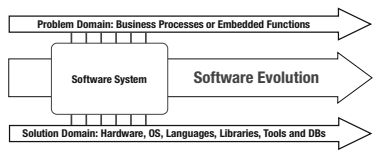
\includegraphics[width=9cm]{Resources/mediator.PNG}
	\caption[نرم‌افزار به عنوان پلی بین دامنه مسئله و دامنه راه‌حل]
	{نرم‌افزار به عنوان پلی بین دامنه مسئله و دامنه راه‌حل
		\cite{wagner_software_2013}؛
		توسعه در یک دامنه، به طور خودکار توسعه در دامنه دیگر را می‌طلبد و در نتیجه می‌باید از فناوری‌ها و تکنولوژی‌ها به نحو احسنت بهره جست تا نیازهای حوزه مسئله را منطبق بر سیستم‌ها و ماشین‌های به روز کرد.
	}
	\label{fig:mediator}
\end{figure}
بسیاری از تحقیقات در سال‌های گذشته، صرف به دست آوردن فرآیندهای نرم‌افزاری با کیفیت شده است؛ البته که فرآیندهای باکیفیت در نهایت منجر به تولید محصولی با کیفیت می‌شود، ولی برای بروز کیفیت در فرآیندها نیز خصیصه‌های کیفی محصول نرم‌افزاری هدف، باید به طور مشخص قید شوند
\cite{sommerville_software_2016}.
هرچند که داشتن یک تعریف مدون و مشخص از کیفیت، لازمه کار هر فرآیند مهندسی نرم‌افزار است، نکته حائز اهمیتی که بسیاری از محققین و پژوهشگران در آثار خود از جمله آقایان پرسمن
\cite{pressman_software_2015}،
سامرویل
\cite{sommerville_software_2016}
و واگنر
\cite{wagner_software_2013}
به آن اشاره کرده‌اند، بیانگر این موضوع است که داشتن یک توصیف کیفیتی  کامل و دقیق از سیستم هدف نیز، به تنهایی، کافی نیست؛ چرا که همین توصیف کیفیتی نیز با گذر زمان، دچار تغییر و تحول خواهد شد و دیگر نیازمندی‌های کیفیتی، معتبر نخواهند بود.\\
همانطور که در شکل
\ref{fig:mediator}
ملاحظه می‌شود، نرم‌افزار میان دو دامنه مسئله و راه‌حل ارتباط برقرار می‌کند و می‌بایست پلی بین فرآیند‌های کسب‌وکاری و پلتفرم‌های فناوری (سیستم‌های عامل، سخت‌افزارها و نرم‌افزارهای مختلف) ایجاد کند. اما توجه به این نکته حائز اهمیت است که هم فرآیندهای کسب‌وکار و هم پلتفرم‌های فناوری، در طول زمان دچار تغییر می‌شوند؛ به خصوص که سرعت تغییرات در عصر حاضر به شدت زیاد است. سخت‌افزارها منسوخ می‌شوند، سیستم‌های عامل به نسخه‌های جدیدتری ارتقا پیدا می‌کنند، زبان‌های برنامه‌نویسی پیشرفته‌تر می‌شوند، ابزارهای جدیدی تولید می‌شوند و کسب‌وکارها در نتیجه این تغییرات، خود را به روز می‌کنند و فرآیندهای کسب‌وکاری نیز می‌بایست بتوانند این تغییرات را پشتیبانی کنند و در نتیجه تغییر می‌کنند
\cite{wagner_software_2013}.\\
در نتیجه ویژگی‌ها و نیازمندی‌های کیفی نرم‌افزار نیز تغییر پیدا می‌کند و اگر خود نرم‌افزار مطابق این تغییرات به روز رسانی نشود، سیستم کم‌کیفیتی خواهیم داشت.
\subsection{تضمین و کنترل کیفیت}
همانطور که پرسمن در کتابش
\cite{pressman_software_2015}
مطرح می‌کند، رسیدن به یک محصول با کیفیت در مهندسی نرم‌افزار، به صورت ضمنی و خود به خود ممکن نیست؛ بلکه نتیجه بازنگری در چهار بعد کلی در فرآیند مهندسی نرم‌افزار و اِعمال مجموعه آن‌ها است:
\begin{itemize}
	\item 
	روش‌های مهندسی نرم‌افزار
	\item 
	تکنیک‌های مدیریت پروژه
	\item 
	فعالیت‌های کنترل کیفیت
	\item
	فعالیت‌های تضمین کیفیت
\end{itemize}
طبق این اظهار نظر، با فرض اِعمال شدن روش‌های درست و بهره‌ور مهندسی نرم‌افزار و تکنیک‌های موثر در مدیریت پروژه تولید نرم‌افزار - که با تقریب خوبی هر دو را می‌توان جزو روش‌های مدیریتی و در حوزه تصمیم‌گیری‌های کلان سیستم دانست - بدیهی است که همچنان کنترل کیفیت و تضمین آن، دو بعد فنی و جزئی‌تر رسیدن به نرم‌افزار با کیفیت را تشکیل می‌دهند. بنابراین می‌بایست روش‌های موثر به منظور انجام فرایند‌های کنترل کیفیت و تضمین رسیدن به آن، توسط تیم مهندسی نرم‌افزار اتخاذ شود.\\
اما، مشابه هر فرایند و فعالیت دیگری، رسیدن به کیفیت نیز هزینه‌های خاص خود را دارد. هزینه کیفیت در نرم‌افزار، مطابق اظهارنظر پرسمن، به سه دسته هزینه‌های پیش‌گیری، هزینه‌های ارزیابی و هزینه‌های خرابی تقسیم می‌شود. هرکدام از این هزینه‌ها، در صورت پیش‌بینی و رفع نواقص محتمل/پیش‌آمده در هر مرحله از طراحی و پیاده‌سازی، بدون اینکه وارد مرحله بعدی شویم، می‌تواند با نرخ بسیار زیادی کاهش یابد 
\cite{pressman_software_2015}.
%\subsection{نقش ابزارها در تامین کیفیت}
%صثثقلثقل
\subsection{کیفیت در سامانه‌های نرم‌افزاری مبتنی بر وب}
یکی از علل عدم رضایت کاربران و مشتریان از وب‌اپلیکیشن‌ها - که درنتیجه این نارضایتی، آمار کاربران وب‌اپلیکیشن‌های کسب‌وکارها دستخوش تغییرات نامطلوب شده و حتی هزینه‌های گزافی به تیم مهندسی نرم‌افزار به خاطر اعمال تغییر پس از تحویل، وارد می‌شود- طراحی نه‌چندان کاربرپسندانه واسط کاربری و زیبایی آن‌هاست 
\cite{agarwal_assessing_2002}؛
بدیهی است که استفاده از مدل‌های فرایندی چابک  و تکراری می‌تواند در کاهش هزینه‌های طراحی مجدد پس از تحویل و یا اعمال تغییر در رابط‌های موجود، موثر باشد
\cite{pressman_software_2015}،
 اما هنوز یک سوال بدون پاسخ خواهد ماند:
 \textit{«چه رابطی برای کاربران وب‌اپلیکیشن (محصول) من مناسب است و طبق نیازمندی‌های فعلی حداکثر کیفیت را تامین خواهد کرد؟»}
 برای پاسخ به این سوال، چک‌لیست‌ها و توصیه‌های فراوانی ارائه شده است
  \cite{pressman_software_2015, sommerville_software_2016}
 که هرکدام به نحوی در افزایش کیفیت رابط‌های کاربری تاثیرگذار بوده‌اند، اما برای تست یک رابط کاربری به صورت کمی، تحلیل و یافتن نقاط ضعف در زیبایی و همچنین ریزبینی در مورد استفاده‌پذیری یک واسط کاربری، به نظر می‌رسد که بررسی بیشتری مورد نیاز است
 \cite{albert_measuring_2013}.
 
 \section{مشخصه‌های کیفی نرم‌افزار}
 \subsection{کارآیی}
 به تعبیر نویسندگان مرجع
 \cite{albert_measuring_2013}
هر کاربر می‌تواند برای خودش تعریفی از کارآیی ارائه نماید. در ادامه بررسی مفصل و مقایسه تطبیقی از مدل‌های کیفی مختلف و کارآیی در هرکدام انجام شده است ولی در اینجا به طور مختصر به ارائه و مقایسه سه نوع دیدگاه از تعریف کارآیی می‌پردازیم:
\begin{enumerate}
	\item 
	سازمان بین‌المللی استانداردها (ایزو ۹۲۴۱-۱۱) کارآیی را در سه حوزه تعریف می‌کند:
	\emph{«میزان سودی که استفاده از یک محصول در رسیدن به اهداف مورد نظر کاربران در رابطه با کاربردی مشخص، که همراه با تاثیرگذاری، بهره‌وری و رضایت باشد، کارآیی آن محصول نامیده می‌شود.»}
	\item
	جامعه متخصصین کارآیی
	\LTRfootnote{Usability Professionals Association}
	بیشتر روی فرایند تولید و توسعه محصول تمرکز می‌کنند و با بیان استفاده‌پذیری به عنوان «یک روش برای کاستن هزینه‌ها و تولید ابزارهایی که مختص کاربرانشان باشد»، از ویژگی مرتبط بودن همواره استفاده‌پذیری با کاربران، استفاده می‌کند.
	\item 
	استیو کورگ در کتاب خود، کاری نکن که من به فکر کردن بیفتم  تعریف عامیانه‌تری را ارائه می‌دهد؛ وی معتقد است که استفاده‌پذیری به معنی اطمینان حاصل کردن از کار کردن خوب محصول نهایی است. با این توضیح که یک فرد با دانش، توانمندی و تجربه کم نیز بایستی بتواند از محصول به راحتی استفاده کند و نیازهای خود را برطرف سازد.
\end{enumerate}
 با بررسی‌های مرجع
 \cite{albert_measuring_2013}
 تمامی تعاریف مطرح برای استفاده‌پذیری، شامل سه زمینه کلیدی و مهم هستند:
 \begin{enumerate}
 	\item 
 	کاربری وجود دارد.
 	\item 
 	این کاربر مشغول انجام کاری است.
 	\item 
 	کاربر در حین کار خود، با یک سیستم یا محصول نرم‌افزاری در تعامل است.
 \end{enumerate}
 یکی از عوامل بسیار تاثیرگذار در استفاده‌پذیری هر محصولی، رابط کاربری آن است؛ از طرفی وجهی که در طرف کاربران قرار دارد و کاربران با آن‌ در ارتباط هستند، در کاربردهای حساس، اهمیتی دو چندان می‌یابد.به عنوان مثال تابلویی که در شکل
\ref{fig:bluffton}
قابل مشاهده است به دلیل استفاده‌پذیر نبودن منجر به تلفات جانی شده. طبق اظهاراتی که در مرجع 
\cite{albert_measuring_2013}
از این حادثه شده است، گرچه استفاده‌پذیری در ابتدا موردی سطحی و غیر ضروری به نظر می‌رسد اما عدم وجود آن در برخی از کاربردهای حساس می‌تواند منجر به آسیب‌ها و خسارت‌های زیادی شود.
\begin{figure}[H]
	\centering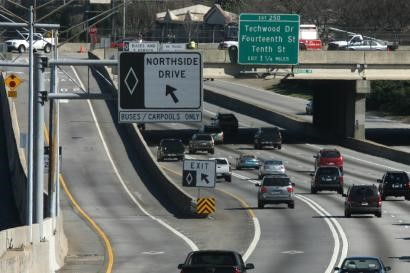
\includegraphics[width=14.8cm]{Resources/tabloo.JPG}
	\caption[تابلویی که نصب نامناسب آن منجر به عدم استفاده‌پذیری و تصادف جاده‌ای شد]
	{تابلویی که نصب نامناسب آن منجر به عدم استفاده‌پذیری و تصادف جاده‌ای شد؛ این تابلو (تابلوی بزرگ سفیدرنگ) که به خاطر نصب در جای نامناسب و استفاده‌پذیری پایینش، راه منتهی به مسیری را نشان می‌دهد که یک طرفه است و در اصل هدف از قرار دادن این تابلو، نشان دادن خروجی در چند متر جلوتر بود
		\cite{noauthor_bluffton_2018}.
	}
	\label{fig:bluffton}
\end{figure}
 اینکه کاربر در طول دوره کاری‌اش با سیستم به طور دقیق به چه موارد منفی یا مثبت یا حتی خنثی برخورده، نقش مهمی در تجربه کاربری وی خواهد داشت.\\
 استفاده‌پذیری به طور کلی به توانایی کاربر در انجام موفق یک کار مشخص دلالت دارد، در حالی که تجربه کاربری به جنبه وسیع‌تری پرداخته و شامل احساسات، عواطف و ادراکات کاربر در حین کار با سیستم می‌شود
 \cite{albert_measuring_2013}.
 در بخش‌های بعدی و با بررسی مدل‌های کیفی مختلف که به منظور سنجش کمی کیفیت نرم‌افزار ارائه شده‌اند، خواهیم دید که استفاده‌پذیری نرم‌افزار، به عنوان یکی از مشخصه‌های اصلی در اغلب این مدل‌ها و به صورت صریح  بیان شده است. با بررسی پژوهش‌ها و کارهای گذشته و همچنین نکاتی از مرجع
 \cite{pressman_software_2015}،
 می‌توان گفت از سال ۱۹۷۰ تا به اکنون، تقریبا در هر مدل کیفی ارائه شده برای نرم‌افزار و به طور خاص برای سامانه‌های کاربری تحت وب، استفاده‌پذیری به صورت صریح به عنوان یک مشخصه اصلی بیان شده است؛ بنابراین می‌توان ادعا کرد استفاده‌پذیری یک نرم‌افزار، از جمله ویژگی‌های مهم کیفی در دستیابی و کنترل کیفیت نرم‌افزار است.
 \subsubsection{استفاده‌پذیری و لایه‌های طراحی سامانه‌های مبتنی بر وب}
 استفاده‌پذیری در وب‌اپلیکیشن‌ها - که امروزه نقش مهمی در ارائه محتوا و سرویس به کاربران دارند - به عنوان یکی از ابعاد و مشخصه‌های اصلی و مهم در کیفیت مطرح است
 \cite{pressman_software_2015}.
رسیدن به کیفیت بالا نیازمند صرف هزینه (تلاش و زمان) است؛ صرفا با در نظر گرفتن بعد کارآیی، پرواضح است که هرچه مشکلات و نواقص رابط‌های کاربری زودتر پیدا شده و مرتفع گردند، با پرداخت هزینه (تلاش و زمان) کمتر به کیفیت بیشتری رسیده‌ایم؛ لایه‌های طراحی سامانه‌های مبتنی بر وب، هر کدام تمرکز جدایی دارند که در ادامه به طور مختصر قید شده‌اند. هر کدام از این لایه‌ها، به نوعی کارآیی نهایی محصول را تامین می‌کنند و در تضمین کیفیت باید به هر لایه به طور جداگانه توجه ویژه‌ای را معطوف نمود.
\section{چرخه طراحی سامانه‌های مبتنی بر وب}
از جمله مراحل هرم طراحی وب‌اپلیکیشن
\cite{pressman_software_2015}،
طراحی واسط کاربری است.  همانطور که در شکل
\ref{fig:pyramid}
مشاهده می‌شود، طراحی زیبایی، محتوا، پیمایش، معماری و همچنین مولفه نیز در فرایند طراحی می‌بایست انجام شوند که هرکدام نکات خاص خود را دارند و می‌توانند در استفاده‌پذیری سامانه کاربردی مبتنی بر وب تاثیرگذار باشند.
\begin{figure}[H]
	\centering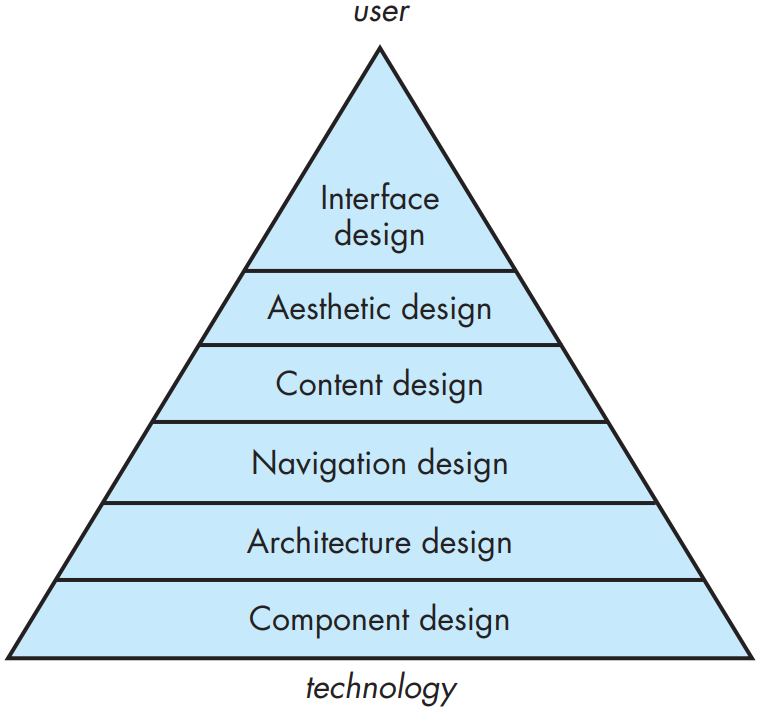
\includegraphics[width=7cm]{Resources/pyramid.PNG}
	\caption[هرم طراحی سامانه‌های مبتنی بر وب]
	{هرم طراحی سامانه‌های مبتنی بر وب
		\cite{pressman_software_2015}
		که نشان‌دهنده لایه‌ها، مراحل و اجزای ساخت یک سامانه مبتنی بر وب است.
	}
	\label{fig:pyramid}
\end{figure}
همچنین شایان ذکر است که لایه‌های مختلف این هرم، هرکدام توجه جداگانه‌ای دارند و می‌بایست در تامین کیفیت، به در هر لایه سیاست‌های به خصوصی اتخاذ شود. قبل از تولید کد وب‌اپلیکیشن، واسط کاربری، به صورت یک نمونه اولیه و در قالب طرح‌های ابتدایی، ماکت‌های مفهومی و یا چارچوب‌های کلی توصیف و طراحی می‌شوند. پس از رسیدن به توافق با مشتری (در صورت نیاز) و یا اعمال تغییرات متعدد تا رسیدن به توافق، این طراحی به کد قابل اجرا و پیاده‌سازی روی وب‌اپلیکیشن تبدیل می‌شود و نهایتا به تولید واسط کاربری آن می‌انجامد
\cite{sommerville_software_2016}.

\begin{figure}[H]
	\centering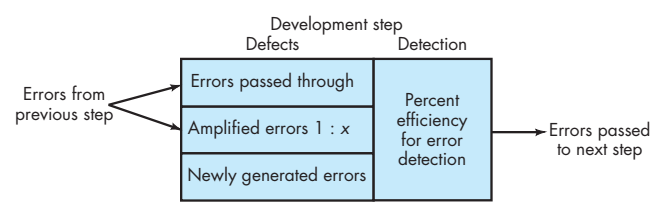
\includegraphics[width=12cm]{Resources/defect.PNG}
	\caption[مدل تشدید خرابی در نرم‌افزار]
	{مدل تشدید خرابی در نرم‌افزار
		\cite{pressman_software_2015}
		نشان‌دهنده تاثیرگذاری خرابی‌های مراحل قبل در هر مرحله از توسعه محصول می‌باشد. طبق این مدل، هرچه بتوان درصد بیشتری از خطاها را هنگام مرور و بررسی هر مرحله شناخت، خرابی‌های کمتری به مراحل بعدی راه پیدا کرده و در نتیجه محصول نهایی با کیفیت‌تر خواهد بود.
	}
	\label{fig:defect}
\end{figure}
مطابق شکل
\ref{fig:defect}
خرابی‌ها و خطاها در صورتی که برطرف نشوند و وارد مرحله بعد شوند، می‌توانند در تولید وب‌اپلیکیشن مشکلات جدی‌ای ایجاد کنند؛ چرا که این خطاها تشدید می‌شوند و دچار خرابی کار سایر لایه‌ها نیز می‌گردند و در نهایت منجر به افت کیفیت محصولات نهایی می‌گردند. از جمله خطاها و خرابی‌های مطرح در حوزه طراحی رابط کاربری، ناکارآمد بودن ایده‌های اولیه و چکش‌نخورده است. مطابق آنچه در قسمت تضمین و کنترل کیفیت گفته شد، در صورت ارزیابی، تحلیل و رفع ایرادات مربوط به استفاده‌پذیری رابط کاربری، در همان مراحل ابتدایی و پس از تولید نمونه‌ اولیه، می‌توان هزینه‌های بعدی را به طور قابل ملاحظه‌ای کمتر کرد.\\
مانند هر روش کیفی دیگری در تضمین کیفیت نرم‌افزار، به منظور دستیابی به استفاده‌پذیری قابل قبول (مطابق نیازهای مشتری) در واسط کاربری وب‌اپلیکیشن‌ها (همچون هر مشخصه اصلی دیگری) می‌بایست فاکتورها، معیارها و مولفه‌های مختلفی به منظور خرد و قابل اندازه‌گیری کردن این مفهوم کلان مطرح شود؛ به طوری که بتوان در قالب مقادیر کمی، نیازمندی‌ها را با داده‌های به دست آمده از ارزیابی رابط کاربری وب‌اپلیکیشن مقایسه و تحلیل کرد. اما در بسیاری از موارد، همانطور که
\cite{agarwal_assessing_2002,p._miguel_review_2014, albert_measuring_2013}
ذکر می‌کنند، حقیقت محض و یا تخمینی تضمین‌کننده‌ای\RTLfootnote{Promising Heuristic}، برای رسیدن به یک رابط کاربری «خوب» وجود ندارد و طراحی‌های استفاده‌پذیر و موثر، موفقیت خود را اغلب یا به روش‌های تجربی، که الزاماً با روش‌های علمی به اثبات نرسیده‌اند، و یا به ذوق هنری طراح مدیون‌اند.
\subsection{تلفیق نگاه مهندسی و هنری}
دور از ذهن نیست که بگوییم یکی از فاکتورهای محبوبیت یک اثر هنری، جذابیت اثر در دید مخاطبانش است. بنابراین پرواضح است که در مورد رابط‌های کاربری، که در ابتدای کار و هنگامی که هنوز توسعه سامانه در فازهای ابتدایی و مذاکرات ابتدایی است به صورت یک طرح مفهومی بوده و اثر یک طراح -که الزاما شاید سررشته‌ای از مهندسی نداشته باشد- هستند، نظر کاربران و استفاده کنندگان آن طرح مفهومی و نحوه تعاملشان با طرح مفهومی، یکی از مشخصه‌های تعیین‌کننده برای موفقیت رابط کاربریِ هدف و تضمین کیفیت آن است.\\
در نتیجه به نظر می‌رسد اندازه‌گیری نظرات کاربران و داشتن یک دید مهندسی در نقطه نظرات کاربران و واکنش‌های آن‌ها هنگام کار با یک طرح مفهومی که به منظور استفاده در یک رابط کاربری ساخته شده است، امری لازم و مثبت خواهد بود و درکل منجر به افزایش اطلاعات تیم طراح و تیم توسعه از نیازهای کاربران خواهد شد.
\section{جمع‌سپاری}
تا سال ۲۰۱۲، با بررسی‌های مرجع 
\cite{estelles-arolas_towards_2012}،
حدود ۴۰ تعریف مختلف در مقالات و پژوهش‌های علمی، حتی گاهی تعاریف متناقض با هم، برای جمع‌سپاری ارائه شده است. نویسندگان آن اثر، با درنظر گرفتن ابعاد مطرح در تعاریف مختلف، در نهایت تعریف نسبتا مفصلی از این مفهوم ارائه می‌دهند که ترجمه آزاد آن در ادامه ذکر شده است: 
\paragraph{جمع‌سپاری}
که ترجمه شده عبارت
\lr{Crowdsourcing}
است، نوعی فعالیت برخط
\LTRfootnote{Online}
مشارکتی است که طی آن یک فرد، یا یک سازمان با ابزارهای کافی به گروهی از افراد با سطح دانش متغیر و گونه‌های متفاوت و با تعداد نامعلومی به انجام فعالیت‌هایی می‌پردازند. در این کار دو سر برد، کارگران انجام دهنده کار
\LTRfootnote{Crowd Workers}
به دلیل داوطلبانه بودن مشارکتشان، از انجام کار خود احساس رضایت می‌کنند؛ چه به خاطر پولی که در ازای انجام کار دریافت می‌کنند و چه به خاطر توسعه مهارت‌های شخصی و یا سایر انگیزه‌ها؛ افراد جمع‌سپارنده هم از مشارکت افراد در حل مسائل پیچیده کمک جسته و سودآوری خود را خواهند داشت. \\
یکی از انگیزه‌های استفاده از جمع‌سپاری، جمع‌آوری داده
\LTRfootnote{Data Collection}
است. در این استفاده، از کارگران جمع‌سپاری شده بهره گرفته می‌شود تا بتوان به مجموعه عظیمی از دیتاست‌ها و یا داده‌های جدید دست پیدا کرد.
\subsection{جمع‌سپاری برای جمع‌آوری داده}
انگیزه اصلی استفاده از جمع‌سپاری در این پروژه، جمع‌آوری داده است. ابزار هدف، قادر خواهد بود تا با استفاده از جمع‌سپاری، بتواند نتایج تست‌های تعریف‌شده توسط مشتریان را از کارگران جمع‌آوری کرده و روی آن‌ها تحلیل و پردازش انجام دهد. عدم وجود یک حقیقت محض قابل اتکا
\LTRfootnote{Ground Truth}
در رابطه با خوب بودن و یا بد بودن یک طراحی رابط کاربری و سلیقه‌ای بودن آن، مهم‌ترین انگیزه استفاده از جمع‌سپاری است؛ همچنین مبتنی بودن تصمیمات و داده‌ها بر داده‌های کاربران مخاطب، می‌تواند منجر به موفقیت حداکثری یک محصول در سازمان شود.\\
همچنین به عنوان یک مهندس، همواره بر آنیم که روش‌های مهندسی و رویکردهای قابل تکرار داشته باشیم. بنابراین نتیجه تلاش در استفاده از یک روش مهندسی برای مدیریت نظرات، استفاده از جمع سپاری خواهد بود.

\chapter{طریقه‌ی مرجع نویسی و واژه‌نامه‌}
\section{طریقه‌ی مرجع نویسی}
برای نوشتن مراجع پایان نامه، برای راحتی کار به صورت زیر عمل می‌کنیم:
\subsection{بارگیری مراجع}
در ابتدا مراجع را باید از سایت‌های معتبر بارگیری کنیم، مثلا برای ارجاع دادن به مقاله‌ی
\lr{A classification of some Finsler connections and their applications}
ابتدا به سایت
\href{scholar.google.com}{گوگل اسکولار} 
رفته و این مقاله را جستجو می‌کنیم. پس از پیدا کردن این مقاله، مانند شکل زیر، در زیر نام و چکیده‌ی مقاله، $5$ گزینه وجود دارد که عبارتند از:\\

\begin{enumerate}
\item \lr{ Cited by}

\item \lr{ Related articles}

\item \lr{ All 6 versions}

\item \lr{ Cite}

\item \lr{ Save}
\end{enumerate}
\begin{figure}[!h]
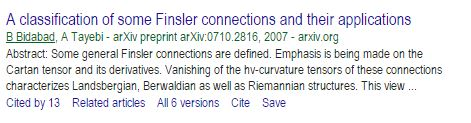
\includegraphics[height=3cm]{bidabad}
\caption{نمونه یک مقاله در گوگل اسکولار}
\end{figure}
در اینجا ما به گزینه‌ی چهارم یعنی
\lr{ Cite}
احتیاج داریم. بر روی آن کلیک کرده و پنجره‌ای مانند
\cref{fig.2}
باز می‌شود که دارای $4$ گزینه‌ی زیر است:
\begin{enumerate}
\item \lr{BibTeX}

\item \lr{EndNote}

\item \lr{RefMan}

\item \lr{RefWorks}
\end{enumerate}
\begin{figure}
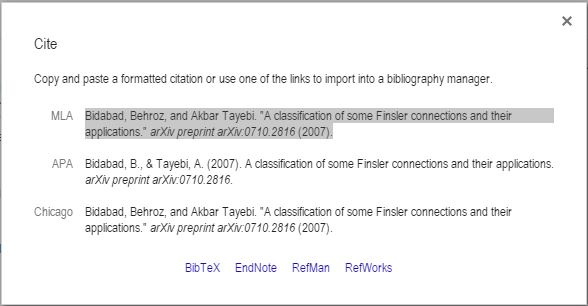
\includegraphics[scale=.6]{bibref}
\caption{پنجره‌ی باز شده در گوگل اسکولار}\label{fig.2}
\end{figure}
روی گزینه‌ی اول، یعنی
\verb;BibTeX;
کلیک کرده و همه‌ی نوشته‌های پنجره‌ی باز شده را مانند زیر، کپی کرده و در فایل
\verb;references.bib;
موجود در فایل
\verb;AUTthesis;
پیست می‌کنیم. سپس کلیدهای
\verb;Ctrl+s;
را می‌زنیم تا فایل ذخیره شود.\\
\begin{latin}
	\normalsize
\begin{verbatim}
@ article{bidabad2007classification,
title={A classification of some Finsler connections and their applications},
author={Bidabad, Behroz and Tayebi, Akbar},
journal={arXiv preprint arXiv:0710.2816},
year={2007}
}
\end{verbatim}
\end{latin}
\subsection{روش ارجاع در متن}
برای ارجاع دادن به مقاله‌ی بالا، باید در جایی که می‌خواهید ارجاع دهید، دستور زیر را تایپ کنید:
\begin{latin}
\lr{$\backslash$cite\{bidabad2007classification\}}
\end{latin}
همانطور که مشاهده می‌کنید از کلمه‌ای که در سطر اول ادرس مقاله آمده (یعنی کلمه‌ی پس از
\lr{@article$\lbrace$})
استفاده کرده‌ایم. پس از دستور فوق، به صورت \cite{bidabad2007classification} و \cite{aa} مرجع خواهد خورد. توجه شود که در صورتی مراجع چاپ خواهند شد که در متن به انها ارجاع داده شده باشد. همچنین برای ارجاع چندتایی از دستور 
\lr{$\backslash$cite\{name1, name2,...\}}
استفاده کنید که به‌صورت \cite{najafi2008finsler, zakeri, najafi} ارجاع خواهند خورد.
\subsection{روش اجرای برنامه}
ابتدا فایل
\verb;AUT_thesis.tex;
را باز کرده و آن را دو بار اجرا کنید. سپس حالت اجرا را از 
\verb;Build Quick;
به حالت
\verb;Bibtex;
تغییر داده و دوباره برنامه را اجرا کنید. دو بار دیگر برنامه را در حالت 
\verb;Build Quick;
اجرا کرده و نتیجه را مشاهده کنید. در این روش تمامی مراجع بر اساس اینکه کدام یک در متن زودتر به آن ارجع داده شده لیست خواهند شد.
\subsection{مراجع فارسی}
برای نوشتن مراجع فارسی باید به صورت دستی، در همان فایل قبلی به صورت زیر عمل می‌کنیم:
\begin{LTR}
\noindent\verb;@article{manifold,;\\
\verb;title={;منیفلد هندسه\verb;},;\\
\verb;author={;بیدآباد دکتربهروز \verb;},;\\
\verb;journal{; امیرکبیر صنعتی دانشگاه\verb;},;\\
\verb;year={1389},;\\
\verb;LANGUAGE={Persian};\\
\verb;};
\end{LTR}
همانطور که مشاهده می‌کنید تنها تفاوت آن با حالت مراجع انگلیسی، سطر آخر آن می‌باشد که زبان را مشخص می‌کند که حتماً باید نوشته شود.
\section{راهنمای واژه‌نامه}

به دلیل پیچیدگی واژه‌نامه‌های موجود در سایت پارسی لاتک، از روش زیر برای نوشتن واژه‌نامه استفاده کنید:

ابتدا با استفاده از اکسل، واژه های خود را یک‌بار براساس حروف الفبای فرسی و بار دیگر انگلیسی مرتب کنید. سپس واژه ها را در فایل \lr{dicen2fa} و \lr{dicfa2en} قرار دهید.

\section{ساخت نمایه}\label{Namaye}
\subsection{ساخت نمایه}
 \begin{enumerate}

\item
کلمات مورد نظر خود مثلا \lr{word} با دستور \verb|\index{word}| ایندکس کنید.
\item
نحوه‌ی اجرای \lr{Make Index}   در ویرایشگرهای \lr{TeX Maker} و \lr{TeX Works}:
\begin{itemize}
\item  تک‌میکر: از منوی \lr{Tools} گزینه‌ی \lr{Xindy Make Index} را کلیک کنید یا از دکمه‌‌های میانبر \lr{Ctrl+Alt+I} استفاده کنید.

\item  تک‌ورکز: ابتدا باید مثل عکس زیر تنظیم  و سپس گزینه‌ی \lr{Xindy Make Index}  انتخاب و روی دکمه‌ی سبز رنگ کلیک کنید یا از دکمه‌های  \lr{Ctrl+T} استفاده کنید.

\begin{figure}[!h]
\centerline{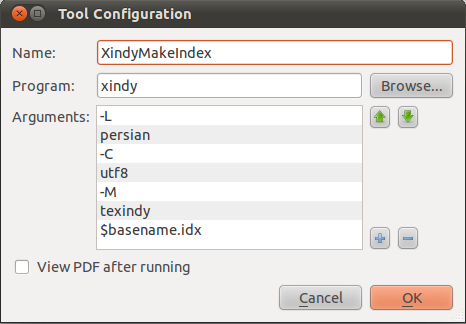
\includegraphics[width=.5\textwidth]{Xindy_Make_Index.png}}
\caption{تنظیمات مربوط به تک‌ورکز}
\end{figure}

\end{itemize}
 \end{enumerate}
 
 \index{کتاب}
\index{پارسی‌لاتک}
\index{بی‌دی}
\index{سوال}
\index{عنصر}
\index{گزینه}
\index{ژاکت}
\index{مرکز دانلود}
\index{اجرا}
\index{تک‌لایو}
\index{ثالث}
\index{جهان}
\index{چهار}
\index{حمایت}
\index{خواهش}
\index{دنیا}
\index{زی‌پرشین}
\index{ریحان}
\index{شیرین}
\index{صمیمی}
\index{ضمیر}
\index{طبیب}
\chapter{مروری بر کارهای گذشته، روش‌ها و ابزارهای موجود}
\section{مدل‌های کیفیتی}
با یک نگاه اجمالی بر منابعی همچون
\cite{wagner_software_2013}،
\cite{seffah_usability_2006}، 
\cite{pressman_software_2015}،
\cite{p._miguel_review_2014}
و همچنین
\cite{sommerville_software_2016}
که به بررسی و مقایسه تطبیقی مدل‌های کیفی پرداخته‌اند، به این نکته پی می‌بریم که صحبت از کیفیت و پژوهش در مورد مدل‌های کیفی از همان ابتدا و به صورت همزمان با پژوهش‌های مربوط به توسعه نرم‌افزار و متدولوژی‌ها مورد توجه بوده است.
در شکل
\ref{fig:qmodels}
ملاحظه می‌شود که از سال ۲۰۰۱، کم‌کم مدل‌های عام‌منظوره‌ای همچون مدل‌های مک‌کال و درومی
\LTRfootnote{Dromey}
کم‌رنگ‌تر شدند و شاهد معرفی شدن مدل‌های خاص‌منظوره بودیم.
\begin{figure}[H]
	\centering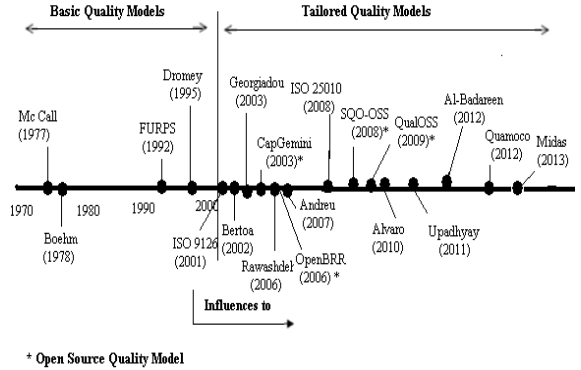
\includegraphics[width=10cm]{Resources/qmodels.PNG}
	\caption[خط زمانی ارائه مدل‌های کیفیتی]
	{خط زمانی ارائه برخی از مدل‌های کیفیتی
		\cite{p._miguel_review_2014}؛
		با پیچیده شدن نیازمندی‌ها و گسترش آن‌ها، دسته‌ای از مدل‌ها تحت عنوان مدل‌های کیفیتی
		\lr{Tailored}
		در شکل مشخص شده‌اند که به طور خاص و برای یک نیازمندی خاصی ساخته شدند، مدل‌های
		\lr{Basic}
		اما به عنوان پایه مدل‌های کیفیتی عمل می‌کندد و تقریبا تمامی مدل‌ها از روی این مدل‌های اصلی اقتباس شده‌اند.
	}
	\label{fig:qmodels}
\end{figure}
مدل‌های عام‌منظوره که در شکل با نام Basic شناخته می‌شوند، ابعاد کلی کیفیت نرم‌افزار را هدف قرار داده‌اند و تقریبا می‌توانند در هر نرم‌افزاری مورد استفاده قرار بگیرند؛ مدل‌های بعدی که ارائه شدند، روی ابعاد خاصی از سازمان یا محصول نرم‌افزاری تمرکز داشته‌اند. این مدل‌ها در نتیجه افزایش پیچیدگی محصولات نرم‌افزاری و فرایندهای سازمانی، برای استفاده در کاربردهای خاص و برای سازمان‌های خاص توسعه داده شدند
\cite{p._miguel_review_2014}.\\
در بررسی مدل‌های کیفی، مرجع
\cite{wagner_software_2013}
دسته‌بندی‌ای را ارائه داده است که بر اساس آن، مدل‌های کیفی را می‌توان به سه دسته سلسله‌مراتبی، مبتنی بر متامدل و همچنین مدل‌های ضمنی تقسیم‌بندی کرد که توضیحات هرکدام در ادامه به صورت مختصر قید شده است.
\subsection{مدل‌های سلسله‌مراتبی}
روش‌های Boehm
\cite{boehm_quantitative_1976}
و مک‌کال
\cite{mccall_factors_1977}
در ارائه مدل کیفی، تشابه زیادی باهم دارند؛ هر دو در خرد کردن مفهوم کیفیت، از یک روش سلسله‌مراتبی استفاده کردند و مطابق شکل
\ref{fig:heir}
کیفیت را به خصیصه‌های مشخصی (که از آن‌ها با نام فاکتورهای کیفیت یاد می‌شود) تقسیم کرده‌اند. این‌گونه مدل‌ها در طول زمان دچار تغییراتی شدند و تفاوت نحوه تقسیم‌بندی آن‌ها، تفاوت مدل‌ها را پدید آورده است.
به تعبیر واگنر
\cite{wagner_software_2013}
رویکرد این نوع مدل‌های کیفی، خرد کردن کیفیت به معیارهای قابل اندازه‌گیری و در نهایت اندازه‌گیری و مقایسه آن‌هاست. همچنین واگنر در بررسی خود، از نقدهایی همچون «مبهم بودن برخی از این تقسیم‌بندی‌ها و شفاف نبودن آن‌ها به طور کامل» یاد می‌کند که از عوامل مهم ناکارآمدی برخی از آن‌هاست؛ همچنین وی در سال ۲۰۱۲ این نکته را متذکر شد که تنها کمتر از ۲۸٪ سازمان‌های فعال در حوزه نرم‌افزار، از مدل‌های استاندارد در تضمین کیفیت فعالیت‌ها و محصولاتشان استفاده می‌کنند و ۷۱٪ این سازمان‌ها، مدل‌های کیفی خود را از روی این مدل‌های کیفی، گلچین کرده و شخصی‌سازی می‌کنند
\cite{wagner_software_2012}.
\begin{figure}[H]
	\centering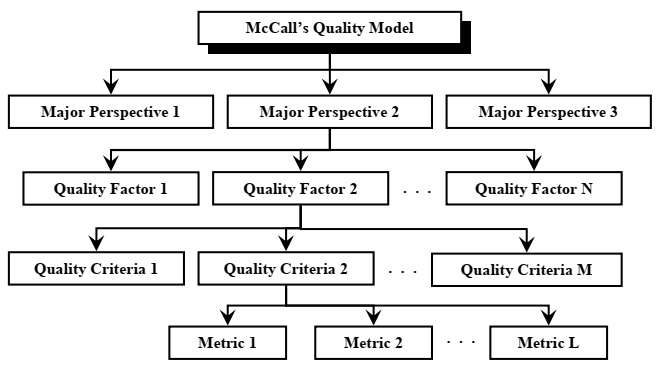
\includegraphics[width=11	cm]{Resources/heir.PNG}
	\caption[ساختار مدل کیفی مک‌کال به عنوان یک مدل کیفی سلسله‌مراتبی]
	{ساختار مدل کیفی مک‌کال به عنوان یک مدل کیفی سلسله‌مراتبی
		\cite{al-qutaish_quality_2010}؛
		این دسته از مدل‌ها کیفیت را به خصیصه‌های خردتری تقسیم می‌کنند و مجددا هر خصیصه را به زیرخصیصه‌های خردتر تقسیم کرده و به همین منوال تا جایی پیش می‌روند که بتوان زیرخصیصه کیفی را به آسانی اندازه‌گیری و شاخصی برای آن تعیین کرد.
	}
	\label{fig:heir}
\end{figure}
همانطور که در شکل
\ref{fig:wagner}
مشاهده می‌شود، طی این بررسی، ۷۹ سازمان مدل‌های کیفیتی شخصی‌سازی‌شده توسط سازمان خود را در اولویت قرار داده و از آن‌ها استفاده می‌کنند. طبق اظهارات این بررسی و همچنین بسیاری از منابع دیگر همچون
\cite{pressman_software_2015} و
\cite{sommerville_software_2016}،
نیاز برای شخصی‌سازی مدل‌های کیفیتی استاندارد وجود دارد. چرا که این مدل‌های سلسله‌مراتبی، به صورت تجریدی بیان شده‌اند و نیازمند دقیق شدن روی متریک‌ها و روش‌های اندازه‌گیری هر متریک هستند.
\begin{figure}[H]
	\centering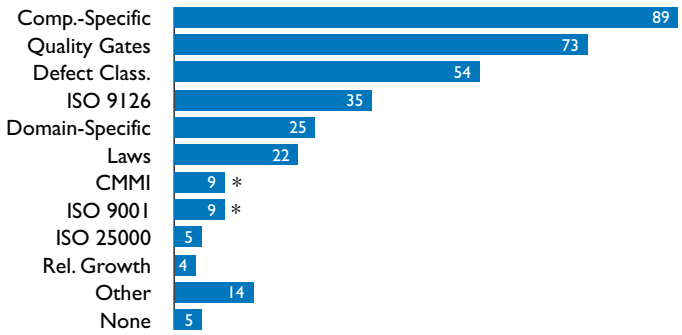
\includegraphics[width=11cm]{Resources/wagner.PNG}
	\caption[بررسی انواع مدل‌ها/رویه‌های کیفیتی استفاده شده در سازمان‌ها]
	{بررسی انواع مدل/رویه‌های کیفیتی استفاده شده در سازمان‌ها
		\cite{wagner_software_2012}؛
		ملاحظه می‌شود که ۸۹ شرکت (اکثریت) فعال در حوزه فناوری اطلاعات در آلمان، به منظور تضمین کیفیت محصولات خود، مدل کیفیتی مختص به خود را توسعه داده‌اند. اما در توسعه این مدل‌ها، همواره مدل‌های اصلی مورد اقتباس واقع شده‌اند و از آن‌ها استفاده شده است.
	}
	\label{fig:wagner}
\end{figure}
\subsection{مدل‌های مبتنی بر متامدل}
با آشکار شدن این نیاز که می‌بایست مدل‌های پایه‌ای را بیشتر شفاف‌سازی کرد و آن‌ها را بر نیازمندی‌ها تطبیق بیشتری داد، ایده ارائه متامدل‌ها مطرح شد. متامدل در اصل مدلی از یک مدل کیفی است؛ قواعد و ساختارهایی که برای توصیف دقیق یک مدل کیفی نیاز داریم (همچون متریک‌ها و نحوه اندازه‌گیری آن‌ها)، توسط متامدل تعیین می‌گردند
\cite{deissenboeck_software_2009}.
به عبارت دیگر، توصیف اینکه چگونه یک مدل کیفی می‌تواند بر نیازمندی‌ها منطبق شود، به عهده متامدل است
\cite{wagner_software_2013}.
درومی به عنوان مثال، در سال ۱۹۹۵، متامدل نسبتا مفصلی ارائه داد که ذیل آن، میان مولفه‌های محصول نرم‌افزاری (که باید حامل کیفیت باشند - مانند کد منبع نرم‌افزار) و ویژگی‌های عملیاتی نرم‌افزار تفاوت و تمایز قائل شد
\cite{dromey_model_1995}.
\subsection{مدل‌های آماری و ضمنی}
این مدل‌ها سعی در ترجمه مفهوم اطمینان‌پذیری سخت‌افزار و استفاده آن در حوزه نرم‌افزار را دارند. ایده اصلی استفاده از این مدل‌ها، مشاهده خرابی‌ها در طول زمان و پیش‌بینی روند رخ دادن خرابی‌ها در آینده است. به منظور دستیابی به خصیصه‌های کیفیتی مشخصی که برای نیازهای توسعه محور بیان شده،در برخی از مدل‌ها سعی شده از داده‌های آماری برای به دست آوردن برخی از ویژگی‌ها و متریک‌ها استفاده شود.\\
به عنوان مثالی برای این نوع مدل‌ها می‌توان به مدل‌های
\textit{رشد اعتمادپذیری}\LTRfootnote{Reliability Growth Models}
\cite{musa_software_2004}
اشاره کرد. مدل‌هایی که از الگوریتم‌ها و روش‌های یادگیری ماشین برای تخمین موارد مختلف، از قبیل مولفه‌های آسیب‌پذیر و یا غیر کارا و مولفه‌هایی که دارای برخی از ویژگی‌های کیفی خاص نیستند نیز از این نوع‌اند که نمونه‌ای از این مدل‌ها در مرجع
\cite{neuhaus_predicting_2007}
تحت عنوان Vulture یاد شده؛ این مدل، از روش‌های یادگیری ماشین و از یک پایگاه دانش آسیب‌پذیری استفاده می‌کند تا در طول زمان و با گسترش نرم‌افزار، بتواند مولفه‌های آسیب‌پذیر نرم‌افزار را پیش‌بینی کند.\\
همچنین به تعبیر مرجع‌های
\cite{sommerville_software_2016}
و
\cite{wagner_software_2013}،
ابزارها و روش‌های مرور، داشبوردهای مدیریتی و مصورسازی داده، ابزارهای شناخت الگوی رخ‌داد خطا در کد منبع نرم‌افزار و چک‌لیست‌ها، که شاید در ظاهر به طور مستقیم ارتباطی با مدل‌های کیفی نداشته باشند، اما در نهایت به یک یا چند متریک کیفی در ذیل یک مدل کیفی ختم می‌شوند؛ این اشاره به مدل‌های کیفی به صورت ضمنی و غیرصریح بوده و اغلب به طور دقیق ارتباط خود با مدل‌ها را مشخص نکرده‌اند. در نتیجه‌ی ‌تمام موارد ذکر شده، تضمین و کنترل کیفیت به واسطه این سازوکارهای غیرصریح و مدل‌هایی که به طور ضمنی مطرح هستند، منجر به پیچیدگی بیشتر و سختی کار خواهد شد.

\section{تمرکز بر استفاده‌پذیری روی مدل‌های کیفیتی}
در جدول
\ref{tab:models}\RTLfootnote{
	متریک‌های ذکر شده در جدول، همگی ترجمه شده عبارات لاتین هستند و در صورت داشتن ابهام در مورد هرکدام می‌توان به
	\hyperref[sec:glossary]{واژه‌نامه}
	رجوع کرد.
}
مقایسه‌ای تطبیقی میان مدل‌های مطرح از سال ۱۹۷۰ تا ۲۰۱۱ انجام شده است که در انجام این مقایسه، به طور خاص، روی خصیصه استفاده‌پذیری این مدل‌ها تمرکز داشتیم. مدل‌های عام‌منظوره در کنار سایر مدل‌ها به مقایسه درآمده‌اند تا خصیصه‌های استفاده‌پذیری در هرکدام از آن‌ها بررسی شود؛ مدل‌های خاص‌منظوره به خاطر نیاز سازمان خاصی به وجود آمده‌اند که مشتریان مخصوص به خود را داشتند که در صورت تعویض محصول و مشتری و استفاده مدل مفروض در یک سازمان دیگر، الزاما به جواب بهینه منتهی نخواهد شد. در حقیقت ویژگی اصلی مدل‌های کیفیتی مبتنی بر متامدل و دلیل گستردگی آن‌ها، متفاوت بودن نیازهای مشتریان و شرایط سازمان‌هاست
\cite{sommerville_software_2016}.\\
ارائه این مدل‌ها تا سال ۲۰۱۳ یکی از موضوعات پرطرفدار و داغ تحقیقاتی بوده اما به طور تدریجی و از سال ۲۰۱۳، با داشتن مراجعی همچون
\cite{albert_measuring_2013}
می‌توان مطالعه استفاده‌پذیری و رسیدن به یک محصول استفاده‌پذیر را با چک‌لیست‌ها و مطالعات آزمایشگاهی نیز تامین کرد. به خصوص که مرجع
\cite{wagner_software_2012}
از کسب‌وکارهای زیادی نام می‌برد که از هیچ‌کدام از مدل‌های کیفیتی ارائه شده پیشین استفاده نمی‌کنند و از قضا سودآوری زیادی نیز دارند و موفقیت محصولاتشان از سایر رقبا بیشتر است. توجه به این نکته حائز اهمیت است که با ارائه و بحث در مورد خصیصه‌هایی همچون خصیصه‌های مطرح در مرجع
\cite{albert_measuring_2013}
می‌توان انواع مطالعات مطرح در حوزه استفاده‌پذیری را انجام داد و تقریبا سناریویی نخواهد ماند که توسط این خصیصه‌ها مورد پوشش واقع نشوند. بنابراین با توجه به جدول
\ref{tab:models}
می‌توان نتیجه‌گیری کرد که این خصیصه‌ها، به طور خاص برای بررسی، مطالعه و در نهایت بیشینه کردن استفاده‌پذیری رابط‌های کاربری و همچنین تجربه کاربری، کفایت می‌کنند.
\begin{longtable}[c]{|c|c|c|C{7cm}|c|}
	\caption[مقایسه تطبیقی مدل‌های کیفیتی ارائه شده با تمرکز بر استفاده‌پذیری]
	{مقایسه تطبیقی مدل‌های کیفیتی ارائه شده با تمرکز بر استفاده‌پذیری\RTLfootnote{
			تمامی متریک‌های درج شده در جدول ترجمه شده عناوین انگلسی آن‌ها در منابع مختلف هستند؛ در نتیجه ممکن است در ابتدا گیج‌کننده به نظر بیایند. به منظور پی بردن به اصل اصطلاحات به
			\hyperref[sec:glossary]{واژه‌نامه}
			رجوع شود.
	}؛
	مدل‌های کیفیتی بسیاری از سال‌های ۱۹۷۰ تا به امروز ارائه شده‌اند که تعداد اندکی از آن‌ها به عنوان مدل‌های اصلی کیفیتی قلم‌داد می‌شوند و سلسه‌مراتبی هستند. این مدل‌های پایه‌ای، در ادامه به عنوان پایه و اساس برای توسعه مدل‌های کیفیتی دیگر (مبتنی برمتامدل) قرار داده شده‌اند که می‌توان گفت شمار زیادی از مدل‌های ارائه شده از این نوع هستند. بر این اساس، مدل‌هایی که بیشترین ارجاع در سال‌های گذشته به آن‌ها وجود داشته را طی این جدول بررسی کرده‌ایم.
}
	\label{tab:models} \\
	\hline
	\multicolumn{5}{| c |}{مقایسه تطبیقی مدل‌های کیفیتی}\\
	\hline
	ردیف & مدل کیفیتی & سال ارائه & متریک‌های استفاده‌پذیری & مرجع \\
	\hline
	\endfirsthead
	
	\hline
	\multicolumn{5}{| c |}{ادامه جدول \ref{tab:models}}\\
	\hline
	ردیف & مدل کیفیتی & سال ارائه & متریک‌های استفاده‌پذیری & مرجع \\
	\hline
	\endhead
	\multicolumn{5}{| c |}{ادامه جدول در صفحه بعد...}\\
	\hline
	\endfoot
	
	\hline
	\endlastfoot
	1 & \lr{McCall} & 1970 & عملیاتی بودن، آموزش، ارتباطاتی بودن & \cite{mccall_factors_1977} \\ \hline
	2 & \lr{Boehm} & 1976 & ترابرپذیری، نگهداری‌پذیری & \cite{boehm_quantitative_1976} \\ \hline
	3 & \lr{IEEE 1061} & 1990 & فهم‌پذیری، آسانی یادگیری، ارتباطاتی بودن & \cite{radatz_ieee_1990} \\ \hline
	4 & \lr{Shackel} & 1991 & تاثیرگذاری، یادگیری‌پذیری، انعطاف‌پذیری، نگرش مثبت & \cite{shackel_usability-context_1991} \\ \hline
	5 & \lr{Bevan} & 1991 & گونه محصول، گونه کاربر، راحتی استفاده، قابلیت پذیرش & \cite{bevan_what_1991} \\ \hline
	6 & \lr{FURPS} & 1992 & فاکتورهای انسانی، زیبایی، مستندسازی، مفاد آموزشی & \cite{grady_practical_1992} \\ \hline
	7 & \lr{Nielsen} & 1994 & یادگیری‌پذیری، بهره‌وری، خاطرسپاری‌پذیری، خطا، رضایت & \cite{nielsen_usability_1994} \\ \hline
	8 & \lr{ISO 9126} & 2001 & درک‌پذیری، یادگیری‌پذیری، عملیاتی بودن، جذابیت، قبول استفاده‌پذیری & \cite{organization_iso/iec_1991}  \\ \hline
	9 & \lr{Bertoa} & 2002 & درک‌پذیری، یادگیری‌پذیری، عملیاتی بودن & \cite{bertoa_quality_2002} \\ \hline
	10 & \lr{Georgiadou} & 2003 & پشتیبانی، یادگیری پذیری، به‌روز بودن مستندات، کمک برخط، سازگاری & \cite{georgiadou_gequamogeneric_2003} \\ \hline
	11 & \lr{Abran} & 2003 & بهره‌وری، تاثیرگذاری، رضایت، یادگیری‌پذیری، امنیت & \cite{abran_usability_2003} \\ \hline
	12 & \lr{Bass} & 2003 & اصلاح‌پذیری، مقیاس‌پذیری، قابلیت استفاده مجدد، کارایی، امنیت & \cite{bass_linking_2003} \\ \hline
	13 & \lr{Schneiderman} & 2005 & زمان آموزش، سرعت کارایی، نرخ خطاهای کاربر، بقای کاربران، رضایت منحصر به فرد & \cite{shneiderman_designing_2004}  \\ \hline
	14 & \lr{Rawashdeh} & 2006 & درک‌پذیری، یادگیری‌پذیری، عملیاتی بودن، پیچیدگی & \cite{rawashdeh_new_2006} \\ \hline
	15 & \lr{ISO 25010} & 2008 & تناسب، شناسایی‌پذیری، یادگیری‌پذیری، عملیاتی بودن، جلوگیری از خطای کاربری، زیبایی رابط کاربری، دسترس‌پذیری & \cite{noauthor_iso_nodate}  \\ \hline
	16 & \lr{Alvaro} & 2010 & درک‌پذیری، یادگیری‌پذیری، عملیاتی بودن & \cite{alvaro_quality_2005, alvaro_software_2010} \\ \hline
	17 & \lr{Alonso-Rios} و بقیه & 2010 & دانایی‌پذیری، عملیاتی بودن، بهره‌وری، استحکام، ایمنی، رضایت منحصر به فرد & \cite{alonso-rios_usability:_2009} \\ \hline
	18 & \lr{Dubey} & 2012 & تاثیرگذاری، بهره‌وری، رضایت، یادگیری‌پذیری & \cite{kumardubey_usability_2012} \\ \hline
	19 & \lr{Tullis} & 2013 & موفقیت‌آمیز بودن وظیفه، زمان انجام وظیفه، خطاها، بهره‌وری، یادگیری‌پذیری، خصیصه‌های موردی، خصیصه‌های خوداعلامی، خصیصه‌های فیزیولوژیکی و رفتاری، خصیصه‌های ترکیبی و مقایسه‌ای، خصیصه‌های وبسایت بلادرنگ، الگوهای‌ مرتب‌سازی  & \cite{albert_measuring_2013} \\ \hline
\end{longtable}
شایان ذکر است که در همه مدل‌های ذکر شده، الزاما به استفاده‌پذیری به عنوان یک خصیصه اصلی در محصول اشاره نشده است؛ در بعضی از مدل‌ها همچون
\lr{ISO 25010}
استفاده‌پذیری یکی از سطوح اصلی بوده، در اولین سطح سلسه‌مراتبی مدل قرار داشته و جزئی از محصول نهایی است و در برخی دیگر همچون
\lr{Boehm}،
به طور صریح و مشخص به استفاده‌پذیری اشاره‌ای نشده است اما در فرآیندهای توسعه محصول روی آن توجه زیادی وجود دارد.\\
همچنین از بررسی مدل‌های کیفیتی مختلف که صرفا برای توسعه سامانه‌های مبتنی بر وب این نتیجه برمی‌آید که هر متامدل می‌بایست در زمینه مربوط به خود مورد استفاده قرار گیرد و نه جای دیگر
\cite{noauthor_measuringu:_2018}.
نتیجه پیشین به این معنی است که در توسعه سامانه‌های مبتنی بر وب، محدوده کاربران، دانش قبلی آن‌ها، تخصص هرکدام، سن و سایر متغیرهای غیرقابل کنترل توسط توسعه‌دهنده نیز در استفاده‌پذیر بودن این سامانه مبتنی بر وب تاثیرگذار است؛ بنابراین در طراحی رابط کاربری هر سامانه مبتنی بر وب، می‌بایست به این نکات نیز توجه داشت و از آخرین توصیه‌های مربوط به توسعه این نوع سامانه‌ها استفاده کرد
\cite{albert_measuring_2013}.
از جمله این توصیه‌ها و پیشنهاد‌های طراحی، توصیه‌های گوگل برای ساخت سامانه‌های کاربردی مبتنی بر وب پیشرو\LTRfootnote{Progressive Web Applications}
\cite{noauthor_progressive_nodate}
است که در سال ۲۰۱۷ مطرح شده و طبق بررسی‌های انجام شده آینده‌ای روشن در انتظار این نوع از سامانه‌های کاربردی است.

\section{مطالعه استفاده‌پذیری و ارزیابی تجربه کاربری}
متریک‌هایی که در مطالعه استفاده‌پذیری و به طور خاص هنگام بررسی تجربه کاربری، اندازه‌گیری می‌شوند و مورد سنجش قرار می‌گیرند داده‌هایی را به دست ما می‌دهند که در بررسی و استفاده از این داده‌ها می‌توان دو رویکرد کلی داشت
\cite{albert_measuring_2013}:
ارزیابی خرد و ارزیابی کلان\RTLfootnote{
	در سال ۱۹۸۶ و طی مقاله‌ای با عنوان «نقش ارزیابی مستمر و چرخشی در طراحی سیستم‌ها برای کیفیت»
	\cite{hewett_role_1986}،
	دو اصطلاح برای مطالعه تجربه کاربری و استفاده‌پذیری
	\lr{Formative}
	و
	\lr{Summative}
	مورد استفاده قرار گرفتند که هر دو از مفاهیم کلاس درسی برداشت شده‌اند؛ یک ارزیابی مستمر
	(\lr{Formative})
	به معنی پرسیدن سوال در سر کلاس درس توسط معلم بوده و به صورت تدریجی و خرد خرد است؛ در حالی که یک ارزیابی  کلان
	(\lr{Summative})
	بررسی‌ای است که در انتهای هر بازه (مثلا هنگام امتحانات پایان‌ترم) و با برگزاری آزمونی خاص، ارزیابی‌ها انجام می‌شوند. در مقاله ذکر شده همچنین این مورد مطرح می‌شود که که ارزیابی مستمر و خرد برای رسیدن به دقت بالا در برآورد نیازهای مشتری، بهتر است؛ چرا که طبق مدل تشدید خرابی و خطا که پیش‌تر بررسی شد، خرابی‌ها هرچه کمتر بوده و نیازمندی‌های مشتری از همان ابتدا در نظر گرفته شوند و برآورده شوند، کیفیتی بیشتر با صرف هزینه‌ای کمتر خواهیم داشت.
}.\\
\begin{figure}
	\centering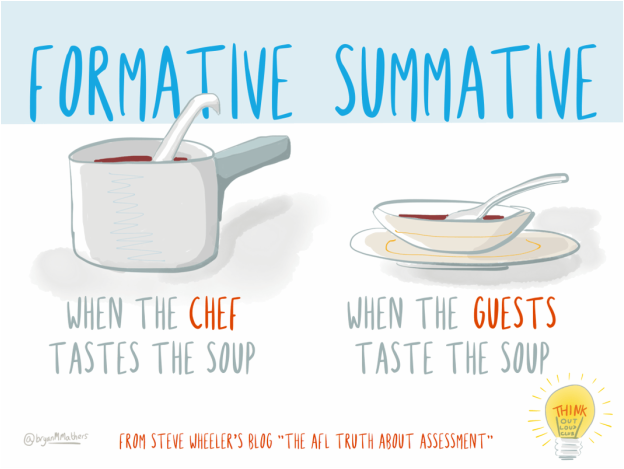
\includegraphics[width=10cm]{Resources/assessment.PNG}
	\caption[مثالی از دو نوع ارزیابی مختلف خرد و کلان]
	{مثالی از دو نوع ارزیابی مختلف خرد و کلان
		\cite{noauthor_formative_nodate}؛
		در این مثال که توسعه‌دهنده نرم‌افزار به آشپز و محصول نهایی به غذای پخته شده توسط آشپز تشبیه شده، تفاوت دو نوع ارزیابی خرد و کلان مطرح شده؛ هنگامی که غذا در حین پخت و توسط آشپز به صورت خرد خرد و در فواصل زمانی کوتاه مورد سنجش قرار می‌گیرد شاهد ارزیابی خرد هستیم و در صورتی که غذا پس از پخت توسط یک منتقد یا مشتری مورد سنجش قرار گیرد، شاهد ارزیابی کلان خواهیم بود.
	}
	\label{fig:assessment}
\end{figure}
همانطور که در شکل
\ref{fig:assessment}
دیده می‌شود، می‌توان این دو نوع ارزیابی را به  چشیدن غذایی بدیل کرد که توسط آشپز و مشتری انجام می‌شوند؛ آشپز در فرآیند پختن غذا به طور مرتب ممکن است غذا را بچشد تا در نهایت خروجی مطلوبی به دست مشتری برسد و غذا از کیفیت لازم برخوردار باشد. در حالی که مشتری در نهایت، محصول نهای را مشاهده می‌کند و صرفا نظر خود در مورد آن غذا و یا کیفیت رستوران را اعلام می‌کند. ذکر این نکته  در همین‌جا خالی از لطف نیست که به وضح می‌توان دریافت که هزینه اعمال تغییرات در صورت درخواست مشتری از آشپز زیاد خواهد بود؛ به طور مشابهی، در صورت عرضه محصول نرم‌افزاری، هزینه تعمیر یک خرابی به مراتب بیشتر از مرور در حین تولید است.
\subsection{ارزیابی خرد}
در یک مطالعه استفاده‌پذیری با رویکرد ارزیابی خرد، محقق به طور مستمر و به صورت دوره‌ای، محصول نهایی را مورد بررسی قرار می‌دهد و در تمامی مراحل تولید نواقص آن را سنجیده و کشف می‌کند و پیشنهاداتی برای رفع آن نواقص ارائه می‌دهد؛ این روند  تا آن جا ادامه پیدا می‌کند که نهایتا یک محصول تقریبا ایده‌آل و یا یک محصول خوب به اندازه کافی\LTRfootnote{
	Good Enough
}
به دست آید. درواقع هدف در این نوع مطالعه هدف بهبود مستمر و رفع ایرادات محصول قبل از عرضه نهایی آن است؛ در نتیجه با بررسی فرآیندهای نرم‌افزاری و همچنین مطالعاتی از قبیل
\cite{sommerville_software_2016}،
\cite{krug_dont_2000} و
\cite{albert_measuring_2013}
به نظر می‌رسد که هرچه ارزیابی خرد زودتر رخ دهد، تاثیر بیشتری روی محصول نهایی و افزایش کیفیت آن خواهد داشت.\\
با اتخاذ این رویکرد، برخی از سوالاتی که می‌توان در فرایند طراحی پرسید عبارتند از:
\begin{itemize}
	\item 
	مهم‌ترین مواردی که کاربران را از رسیدن به اهدافشان منع می‌کند و یا به عدم کارایی آن‌ها می‌شود چیست؟
	\item 
	نقاط قوت و ضعف محصول از نقطه نظر کاربران چیست؟
	\item 
	اشتباهات متداول کاربران هنگام کار با محصول حول چه مواردی است؟
	\item 
	آیا بهبودهای مطرح شده توسط محققین تجربه کاربری، در هر نسخه از طراحی رابط کاربری، مورد استفاده و توجه قرار می‌گیرند؟
	\item 
	پس از عرضه نهایی محصول، چه مواردی در رابطه با استفاده‌پذیری به نظر می‌رسد که هنوز جای کار خواهد داشت؟
	
\end{itemize}
شایان ذکر است که در صورتی که فرصت اصلاح طراحی واسط کاربری وجود نداشته باشد، استفاده از این روش ارزیابی به نظر می‌رسد که کارایی چندانی نداشته باشد و بیشتر باعث هدررفت منابع شود.
\subsection{ارزیابی کلان}
در این روش، محقق همچون یک منتقد، محصول نهایی را از زوایای مختلف مورد بررسی قرار می‌دهد و حتی با محصول‌های دیگر مقایسه می‌کند تا نقدی بر آن وارد سازد. نکته حائز اهمیت این است که در اینجا محصول ارائه شده است و دیگر در فاز توسعه و تولید نیست. هدف از انجام این نوع ارزیابی، پی بردن به این نکته است که این محصول خاص چه‌قدر خوب می‌تواند به نیازمندی‌های کاربران پاسخ دهد و به چه میزان با آن‌ها هم‌جهت است. بر خلاف ارزیابی خرد، این روش، مبتنی بر اصول و قواعد و چک‌لیست‌های مشخصی است که در نهایت محصول با آن‌ها بررسی می‌شود. در مقایسه محصولات مختلف نیز مجددا این اصول و قواعد مبنا قرار می‌گیرند. با بررسی منابع مختلفی از قبیل
\cite{sommerville_software_2016} و
\cite{pressman_software_2015}
می‌توان به این نکته پی برد که سوالاتی از قبیل سوالات زیر بیشتر مناسب انجام این نوع ارزیابی هستند:
\begin{itemize}
	\item 
	آیا اهداف استفاده‌پذیری پروژه (مطرح شده در نیازمندی‌های پروژه) رعایت شده‌اند؟
	\item 
	استفاده‌پذیری کلی سیستم در چه سطحی است؟
	\item 
	نقاط ضعف و قوت محصول مورد نظر در مقایسه با سایر رقبا چیست و چگونه می‌توان در صورت داشتن ضعف، آن را ارتقا داد؟
	\item 
	آیا بهبودهای مطرح برای هر نسخه از نرم‌افزار، پس از عرضه نسخه جدید، اعمال می‌شوند؟
\end{itemize}
در نهایت فراموش نکنیم که همواره تغییر نیازمند صرف هزینه و زمان است؛‌ بنابراین در صورت استفاده از این روش ارزیابی می‌بایست در نظر داشت که برخی فعالیت‌های پسا ارزیابی نیز باید در پس ذهن مدیر پروژه باشد؛ چرا که ممکن است حتی در صورت نیاز پروژه‌ای برای برطرف کردن مشکلات استفاده‌پذیری یک سیستم تعریف شود که خود این پروژه هزینه‌بر باشد.
\subsection{اهداف کاربری}
سوالاتی همچون «آیا محصول مورد نظر نیاز روزانه کاربران را برآورده خواهد کرد و کاربران به طور متداول با این محصول نرم‌افزاری در ارتباط خواهند بود؟» و نیز «آیا کارایی کاربران و بهره‌وری آن‌ها در طول انجام یک وظیفه مشخص در هنگام کار با این نرم‌افزار مهم است؟ چگونه می‌توان آن را بهبود داد؟» به قسمتی از محصول توجه دارند که با نیازمندی‌های کاربر درگیر است. با بررسی‌ مراجعی همچون
\cite{albert_measuring_2013}،
\cite{noauthor_measuringu:_2018}،
\cite{hewett_role_1986} و
\cite{abran_usability_2003}
می‌توان به این نکته پی‌برد که همه این قبیل سوالات که به نیازهای ضمنی و نه الزاما صریح کاربر، در تعامل با رابط کاربری می‌پردازند، به دو متریک اساسی و قابل اندازه‌گیری از نیاز کاربران اشاره می‌کنند\RTLfootnote{
	البته باید توجه کرد که کارایی کاربر و رضایت کاربر در اینجا اشاره به دید کاربر به سامانه هدف دارند و نه اینکه متریک‌های اصلی مدل کیفیتی باشند. در اینجا کارایی و رضایت از دید کاربر و به عنوان نظر وی در مورد سامانه، مورد نظر هستند.
}: کارایی\LTRfootnote{Performance} و رضایت کاربر\LTRfootnote{Satisfaction}.
\paragraph{کارایی}
به عنوان یک متریک کیفیتی به طور خاص در رابطه با تجربه کاربری، به اندازه‌گیری توانایی کاربران در انجام وظایف مشخصی می‌پردازد؛ در این راستا، اندازه‌گیری‌های جنبی نیز اهمیت زیادی پیدا می‌کنند. از جمله این اندازه‌گیری‌ها می‌توان به موارد زیر اشاره کرد که به طور غیر مستقیم در کارایی تاثیرگذار هستند:
\begin{itemize}
	\item 
	زمان سپری شده برای انجام وظیفه
	\item 
	میزان تلاش برای انجام وظیفه (برای مثال تعداد کلیک‌ها و یا توان ذهنی مصرف شده)
	\item 
	زمانی که طول می‌کشد تا کاربر با وظیفه آشنا شود و بدون صرف تلاش خاصی آن را انجام دهد (یادگیری)
\end{itemize}
اندازه‌گیری‌های مربوط به متریک کارایی یک رابط کاربری، اهمیت زیادی دارند چرا که اگر کاربران نتوانند وظایف اصلی در رابطه با تعامل با سیستم را به درستی و با موفقیت به انجام برسانند، در عمل محصول نرم‌افزاری به شکست منتهی شده است و یا حداقل رابط کاربری خوبی ندارد و امکان تعامل موفق کاربر وجود نخواهد داشت.
\paragraph{رضایت}
درواقع نظر نهایی کاربر در مورد تعاملش با سیستم است؛ قضاوتی که کاربر در مورد سیستم و نحوه تعاملش با آن می‌کند می‌تواند با جملات مختلفی مانند «استفاده از آن سخت/آسان بود»، «گیج‌کننده/ساده بود» و ... بیان شود. البته که این تعبیرات غیردقیق هستند اما می‌توان با اعطای درجه‌های آزادی خاصی به کاربران، در حین تعامل با سیستم برخی از متریک‌ها را از آن‌ها به طور خوداعلامی\LTRfootnote{Self-reported Metrics} از کاربران گزارش عددی گرفت؛ چه بسا که به گفته مراجعی همچون
\cite{albert_measuring_2013}،
\cite{alonso-rios_usability:_2009} و
\cite{seffah_usability_2006}
این متریک‌ها در سامانه‌های کاربردی مبتنی بر وب - که هدف اصلی این پروژه هستند - بسیار مهم و تاثیرگذارند. اما باید به این نکته توجه کرد که در محدوده سامانه‌های مبتنی بر وب، رضایت کاربر الزاما همیشه همراه با کارایی حداکثری وی در تعامل با سامانه نیست؛ فاکتورهای بسیاری از قبیل زیبایی و وجود تکنولوژی‌های مختلف، بر این رضایت تاثیر مستقیم دارند و چه بسا که کاربری با رضایت حداکثری از یک سامانه استفاده کند ولی کارایی عملیات وی بسیار پایین باشد.\\
ویژگی‌های محصولی که کاربر با آن در تعامل است به عنوان یکی از اصلی‌ترین مدخل‌ها به بحث رضایت کاربری اهمیت دارند. در درجه دوم اما، کیفیت تعامل به عوامل دیگری همچون دانش قبلی کاربر و سن و جنسیت و غیره وابسته است. در ادامه مدلی برای تشخیص دادن ویژگی‌های محصول نهایی و اینکه کدام یک از آن‌ها و در چه شرایطی منجر به رضایت کاربری خواهند شد معرفی می‌شود.
\paragraph{مدل کانو}
که در سال ۱۹۸۴ و توسط آقای کانو
\cite{kano_attractive_1984}
برای تمییز دادن ویژگی‌های اشتیاق‌برانگیز و صریح و همچنین ویژگی‌های ضمنی و بایدی یک محصول، ارائه شد. طی این مدل، کیفیت محصول نهایی در گرو پنج دسته از نیازمندی‌های زیر است که رسیدن به هر دسته از این‌ها نیازمند اتخاذ سیاست‌های مختلف در طول ساخت محصول است:
\begin{figure}[H]
	\centering
	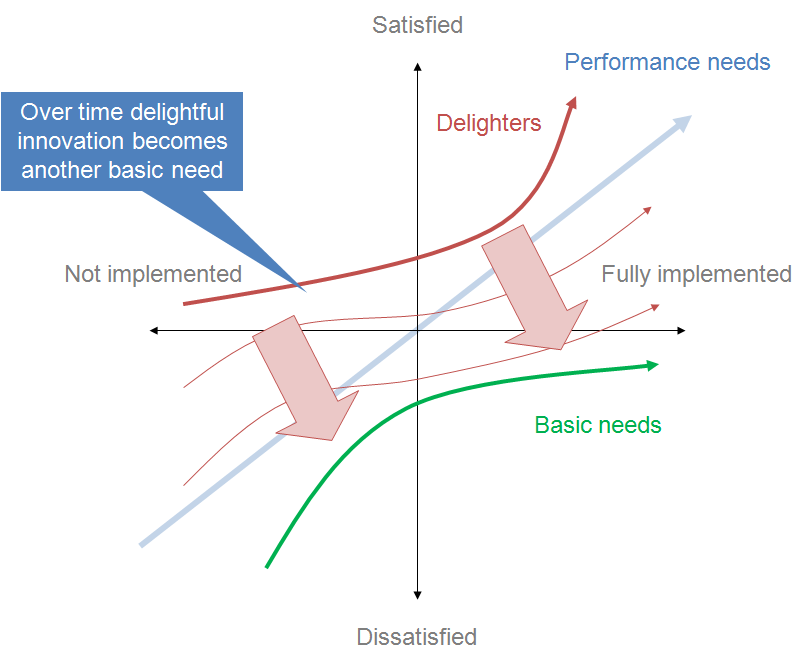
\includegraphics[width=9cm]{Resources/kano_model.PNG}
	\caption[تعبیری از مدل کانو]	{
		تعبیری از مدل کانو
		\cite{noauthor_kano_2018}
	}
	\label{fig:kano}
\end{figure}
\begin{itemize}
	\item 
	نیازمندی‌های بایدی: که مشتریان به طور ضمنی خواستار آن‌ها هستند و ممکن است صریحا بیان نشوند. به عنوان مثال اینکه یک سامانه کاربردی مبتنی بر وب همیشه با یک آدرس اینترنتی خاص
	\lr{URL}
	در دسترس باشد.
	\item
	نیازمندی‌های تک‌بعدی: که در صورت وجودشان کاربر احساس رضایتمندی و در صورت عدم وجودشان در محصول نهایی، کاربر احساس عدم رضایت از محصول را خواهد داشت. برای نمونه می‌توان به واکنش‌گرا بودن یک سامانه مبتنی بر وب روی پلتفرم موبایل اشاره کرد؛ که گفتنی است این روزها به یکی از ویژگی‌های اصلی موفقیت بسیاری از کسب‌وکارهای فعال در ایران تبدیل شده است.
	\item 
	نیازمندی‌های اشتیاق‌برانگیز: که در صورتی که به طور کامل پیاده‌سازی شوند، منجر به رضایتمندی کاربران خواهند شد ولی در صورت عدم پیاده‌سازی، رضایت کاربران از بین نخواهد رفت. به عنوان مثال اینکه یک سامانه پست الکترونیکی مبتنی بر وب\LTRfootnote{Webmail} در کنار لیست ایمیل‌های دریافتی، وضعیت آب‌وهوا و زمان فعلی و گزیده‌ای از اخبار را نشان دهد می‌تواند یک ویژگی اشتیاق برانگیز باشد.
	\item 
	نیازمندی‌های بی‌تفاوت: بودن و نبودنشان تفاوتی در رضایت مشتری نخواهد کرد. به عنوان مثال در بسیاری از پروژه‌های منتهی به یک سامانه کاربردی مبتنی بر وب، پلتفرم و زبان مورد استفاده برای توسعه سامانه، تفاوتی در رضایت مشتریان ایجاد نخواهد کرد.
	\item 
	نیازمندی‌های معکوس: به دسته‌ای از نیازمندی‌ها اشاره دارد که پرداختن بیش‌ازحد به آن‌ها باعث کاهش رضایت کاربران می‌شود. به عنوان مثال برخی از کاربران ممکن است از ابزارهایی که امکانات زیادی به آن‌ها در داشبورد مدیریتی می‌دهند خوششان بیاید و در مقابل برخی از کاربران از پیچیدگی بیش از حد ابزار گلایه کنند.
\end{itemize}
در شکل
\ref{fig:kano}
ملاحظه می‌شود که بسیاری از ویژگی‌های جذاب محصول که هنوز به عنوان نیازمندی مطرح هستند و هنوز پیاده‌سازی نشده‌اند و درنتجیه کاربر امکان انجام عملیات مورد نظر خود را ندارد، انگیزه‌ای برای ساخت سامانه هستند و پس از اینکه این ویژگی‌های عملیاتی (منحی قرمز رنگ) در محصول پدیدار می‌شوند، رضایت کاربران از محصول افزایش پیدا می‌کند؛ گرچه الزاما شاید این ویژگی‌ها، کارایی بالایی از دید کاربران نداشته باشند. به مرور زمان که فناوری پیشرفت می‌کند، نیازمندی‌های فعلی آهسته آهسته به باید‌های سامانه تبدیل می‌شوند (منحنی سبز رنگ).\\
همچنین در مرجع
\cite{sauerwein_kano_1996}
از خط آبی قابل مشاهده در شکل
\ref{fig:kano}،
به عنوان نیازمندی‌های تک‌بعدی یاد شده است که مشتری فقط به طور صریح و مشخص، این دسته از نیازمندی‌ها را مطرح می‌کند و بقیه نیازمندی‌ها معمولا به طور ضمنی مطرح می‌شوند؛ در نتیجه نقش تجربه در مهندسی نرم‌افزار و تولید سیستم‌های باکیفیت را می‌توان کمابیش مشاهده کرد؛ هرچه دانش بیشتری به بدیهیات و سهل‌های ممتنع موجود در نیازمندی‌ها داشته باشیم و اظهارمندی نیازمندی شفاف و مدون‌تری در دست باشد، محصول نهایی با کیفیت‌تر و هزینه و وقت صرف شده کم‌تر خواهد بود.\\
\begin{figure}[H]
	\centering
	\subfloat[تاثیر نیازمندی‌های اشتیاق‌بر‌انگیز]{
		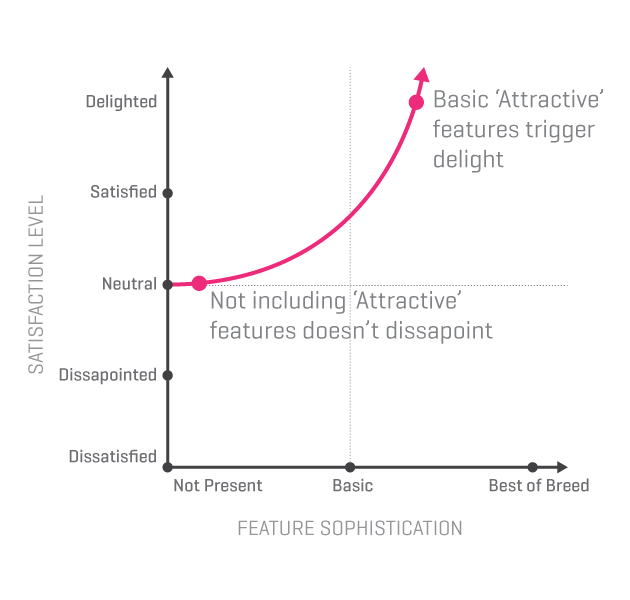
\includegraphics[width=5.5cm]{Resources/kano_attractive.PNG}
	}
	\subfloat[تاثیر نیازمندی‌های تک‌بعدی]{
		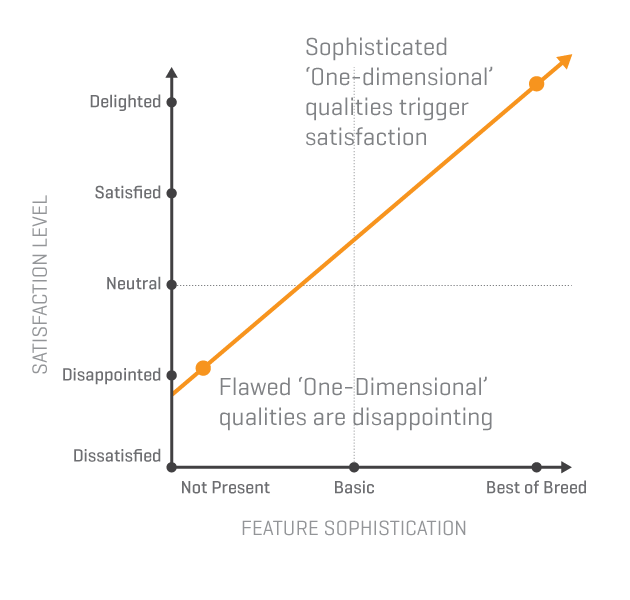
\includegraphics[width=5.5cm]{Resources/kano_one.PNG}
	}
	\hspace{0mm}
	\subfloat[تاثیر نیازمندی‌های بایدی]{
		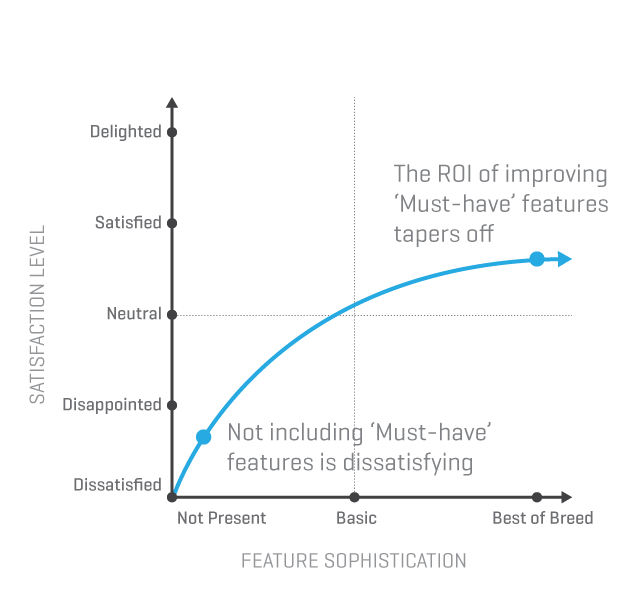
\includegraphics[width=5.5cm]{Resources/kano_must.PNG}
	}
	\subfloat[تاثیر نیازمندی‌های بی‌تفاوت]{
		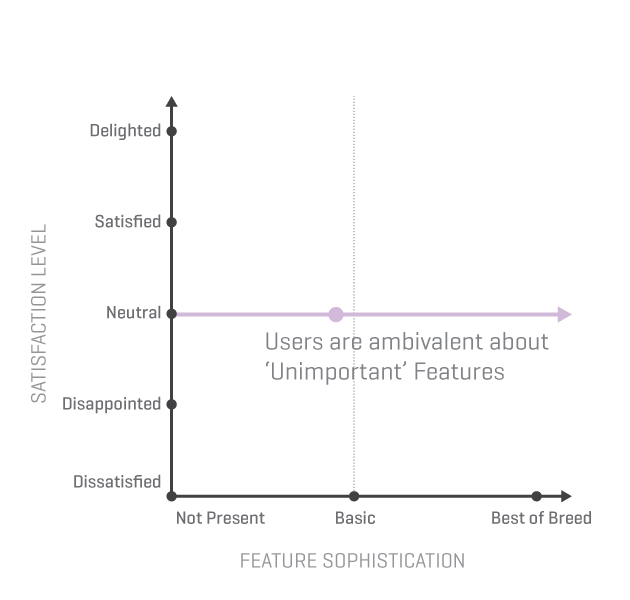
\includegraphics[width=5.5cm]{Resources/kano_unimportant.PNG}
	}
	\hspace{0mm}
	\subfloat[تاثیر نیازمندی‌های معکوس]{
		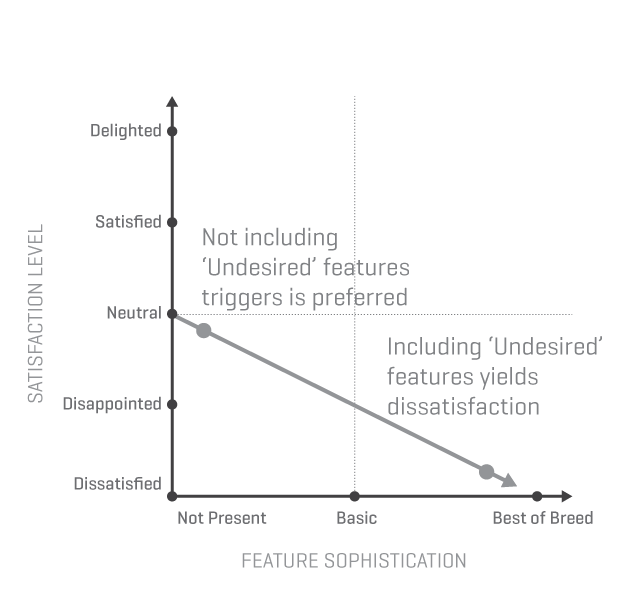
\includegraphics[width=5.5cm]{Resources/kano_undesired.PNG}
	}
	\subfloat[تجمیع نیازمندی‌ها و تاثیرگذاری آن‌ها روی رضایت مشتریان]{
		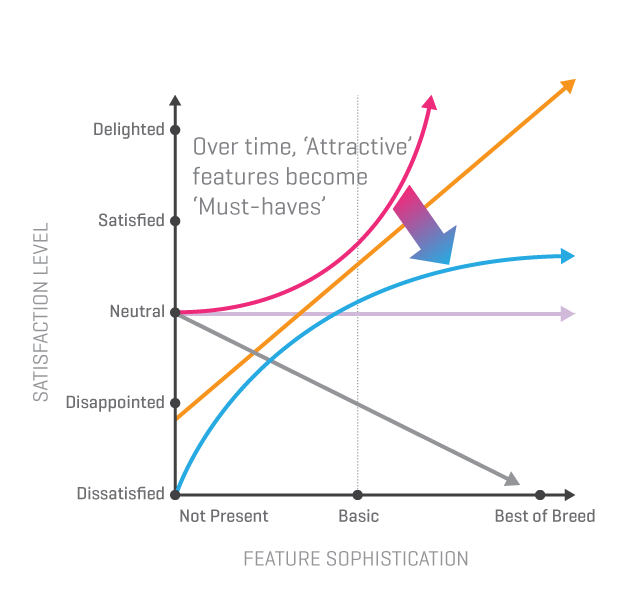
\includegraphics[width=5.5cm]{Resources/kano_model2.PNG}
	}
	\caption[تفسیری از مدل کانو]
	{تفسیری از مدل کانو که نشان‌دهنده ارتباط رضایت کاربر و ویژگی‌های محصول است
		\cite{noauthor_leveraging_2012}؛
		نیازمندی‌های اشتیاق‌برانگیز کاربر، خواسته کاربران نیست ولی در صورت پیاده‌سازی موفق، موج بزرگی از رضایت را در بر خواهد داشت (آ). نیازمندی‌های تک‌بعدی در صورت عدم پیاده‌سازی، موجب نارضایتی خواهد بود (ب). نیازمندی‌های بایدی که درواقع خواسته اصلی کاربران بوده و باید به طور کامل پیاده‌سازی شوند تا رضایت حداقلی کسب شود (ج). نیازمندی‌های بی‌تفاوت نیز بود و نبودشان در محصول نهایی تفاوتی در رضایت مشتری ایجاد نخواهد کرد (د). نیازمندی‌های معکوس نشان داده‌اند که هرچه بیشتر به آن‌ها پرداخته شود، باعث بروز نارضایتی بیشتری خواهند شد (ه). در واقع هر ویژگی‌ای از محصول نهایی، مادامی که پیاده‌سازی نشده است، دچار انگیزش کاربر می‌شود. نیازمندی‌های تکبعدی پس از اینکه به کاملی پیاده‌سازی شد و کاربر از آن استفاده کرد، دچار افزایش رضایتمندی کاربر شده و در نهایت و پس از گذشت اندک زمانی، این ویژگی به یک ویژگی بایدی تبدیل می‌شود که کاربر حتی شاید به طور صریح به آن اشاره نکند ولی نبود آن در محصول باعث عدم رضایتمندی خواهد شد (و).
	}
	\label{fig:kano2}
\end{figure}
تعاریف انواع نیازمندی‌های مطرح شده توسط کانو به جهت اهمیتی که در شناخت خصیصه‌های کیفیتی این پروژه دارند، بار دیگر در شکل
\ref{fig:kano2}
ذکر شده است. مطابق این شکل، ممکن است با برهم زدن معاملات و همواره با تحویل دادن نیاز‌مندی‌های شگفت‌انگیز، مشتریان خود را غافل‌گیر کنیم و برای کسب رضایت موقتی، آن‌ها را از نیازمندی‌های اصلی دور کنیم، اما باید همواره در خاطر داشت که این استراتژی محکوم به شکست است چرا که محلول زمان در نهایت اشتیاق کاربران را در خود حل کرده و غافل‌گیری‌های دیروز تبدیل به باید‌های امروز خواهند بود و دیگر نمی‌توان ارزش افزوده‌ای نسبت به سایر رقیبان و یا نسبت به وضعیت دیروز سازمان خودمان، ارائه داد.\\
نتیجه نهایی از دو بحث پیشین در مورد رضایت کاربر از سامانه و کارایی کاربر در تعامل با سامانه، اینکه این دو خصیصه الزاما دارای همبستگی خاصی نیستند؛ ولی همواره باید در اندازه‌گیری استفاده‌پذیری مدنظر قرار بگیرند چرا که طبق تعریف استفاده‌پذیری، در یک سیستم استفاده‌پذیر، کاربر می‌بایست در نهایت از سیستم راضی بوده باشد و تجربه کاربری خوبی (کارایی در هنگام استفاده از محصول) داشته باشد.
\section{سناریو‌های سنجش استفاده‌پذیری و خصیصه‌های هرکدام}
با مقایسه تطبیقی انجام شده در جدول
\ref{tab:models}
در رابطه با مدل‌های کیفیتی مختلف و همچنین با بررسی مراجعی همچون
\cite{wagner_software_2012}،
\cite{wagner_software_2013} و
\cite{albert_measuring_2013}
می‌توان نتیجه گرفت که در زمان انتخاب خصیصه‌های اندازه‌گیری استفاده‌پذیری در یک محصول (و نه الزاما یک محصول نرم‌افزاری)، می‌بایست به نکاتی از قبیل اهداف مطالعه استفاده‌پذیری\RTLfootnote{اینکه برای ارتقای محصول نهایی و ساخت یک نسخه دیگر است یا برای پیشگیری از بروز خرابی‌های بعدی و ...}، اهداف کاربری محصول\RTLfootnote{اینکه کاربر چه هدفی را از استفاده کردن از این محصول دنبال می‌کند}، فناوری‌ها و ابزارهای موجود برای جمع‌آوری داده و همچنین بودجه و زمان موجود برای تحقیق درباره استفاده‌پذیری، می‌بایست توجه کرد.\\
به تعبیر مرجع
\cite{albert_measuring_2013}،
در دنیای کنونی که نیازمندی‌ها بسیار گسترده و مفصل شده‌اند و جزئی‌ترین تغییرات در نیازمندی‌های مشتری ممکن است دامنه و حوزه مخاطبان یک سامانه را عوض کند و همچنین از آن‌جایی که در هر مطالعه استفاده‌پذیری، ویژگی‌ها و خصیصه‌های خاص آن مطالعه مدنظر قرار می‌گیرند -که الزاما با اهداف سایر مطالعات استفاده‌پذیری یکسان نیستند- نمی‌توان مجموعه‌ای از متریک‌های مشخص و شسته‌رفته‌ای برای اندازه‌گیری و سنجش استفاده‌پذیری در تمام سامانه‌های کاربردی مبتنی بر وب ارائه داد؛‌
در حقیقت، طبق ادعای مرجع
\cite{wagner_software_2012}
بیش از ۷۰٪ سازمان‌های فعال در حوزه فناوری اطلاعات، به منظور تامین و تضمین کیفیت در محصولات نرم‌افزاری خود، مدل‌های گلچین شده و سفارشی‌سازی شده خود را استفاده می‌کنند. بنابراین این پندار که برای تمامی سامانه‌های مبتنی بر وب می‌توان یک مدل کیفیتی ثابت ارائه کرد، غیرمنطقی به نظر می‌رسد. در عوض می‌توان با بررسی سرگذشت تاریخی مدل‌های کیفی و از طریق مقایسه تطبیقی آن‌ها در جدول
\ref{tab:models}
و نیز مطالعه مراجع مختلفی همچون
\cite{alonso-rios_usability:_2009}،
\cite{bass_linking_2003}،
\cite{bevan_what_1991}،
\cite{pressman_software_2015}،
\cite{sommerville_software_2016}
و
\cite{albert_measuring_2013}
که در زمینه تجربه کاربری و استفاده‌پذیری نتایج تحقیقات ارزشمندی را ارائه کرده‌اند، به این نتیجه دست یافت که دسته‌بندی‌های کلی‌ای از انواع مطالعات استفاده‌پذیری می‌توان ارائه نمود، که در هر دسته، با توجه به اهداف و نتایج مورد نیاز مطالعه، متریک‌های خاصی اهمیت بیشتری پیدا می‌کنند و می‌توان به آن‌ها پرداخت.\\
یکی از انواع متامدل‌ها که بر مبنای مدل‌های سلسه‌مراتبی و به طور خاص برای استفاده‌پذیری سامانه‌های کاربردی مبتنی بر وب ساخته شده است در مرجع
\cite{albert_measuring_2013}
ذکر شده است\RTLfootnote{
	البته تمامی خصیصه‌های مطرح برای استفاده‌پذیری در این مدل به طور کامل شرح و بسط داده نشده‌اند؛ چرا که به گفته ارائه دهنده، بسیاری از اقدامات به زمینه مورد مطالعه و تست وابسته بوده و در نتیجه مشخص کردن جزییات نهایی با تیم تضمین کیفیت (تست و ارزیابی استفاده‌پذیری) است. همچنین شایان ذکر است که هیچگاه منبع ذکر شده از خصیصه‌هایی که عنوان کرده به عنوان یک چارچوب و یا متامدل یاد نکرده است؛ اما به جهت اهمیت استدلال و بررسی‌های این منبع و همچنین ارجاعات زیاد به آن، چه در صنعت و ابزارهایی همچون
	\lr{UsabilityHub}
	و چه در دنیای تحقیقات، اهمیت این خصیصه‌های کیفیتی را به عنوان یک متامدل کیفیتی دو چندان می‌کند.
}.
با بررسی‌های انجام گرفته روی انواع مدل‌های کیفیتی عام و خاص منظوره که در موقعیت‌های مختلف ارائه شده‌اند، ده سناریوی مهم برای مطالعه استفاده‌پذیری در وب‌اپلیکیشن‌ها مطرح هستند؛ که می‌توان عناوین هرکدام و خصیصه‌های مناسب هر سناریو را در جدول
\ref{tab:10usability}
مشاهده کرد. در ادامه به بررسی هرکدام از این ده سناریو می‌پردازیم.
\begin{table}[H]
	\caption[سناریوهای متداول مطالعه استفاده‌پذیری و متریک‌هایی که می‌توان برای هرکدام در نظر گرفت]{
		سناریوهای متداول مطالعه استفاده‌پذیری و متریک‌هایی که می‌توان برای هرکدام در نظر گرفت
		\cite{albert_measuring_2013}
	}
	\label{tab:10usability}
	\centering
	%	\resizebox{\textwidth}{!}{%
	\begin{tabular}{|C{5cm}|c|c|c|c|c|c|c|c|c|c|c|}
		\hline
		‏هدف و سناریوی مطالعه استفاده‌پذیری
		& 
		\rotatebox{90}{‏موفقیت‌آمیز بودن وظیفه}
		& 
		\rotatebox{90}{زمان انجام وظیفه}
		& 
		\rotatebox{90}{خطاها}
		& 
		\rotatebox{90}{بهره‌وری}
		& 
		\rotatebox{90}{یادگیری‌ پذیری}
		& 
		\rotatebox{90}{خصیصه‌های موردی}
		& 
		\rotatebox{90}{خصیصه‌های خوداعلامی}
		& 
		\rotatebox{90}{خصیصه‌های فیزیولوژیکی و رفتاری}
		& 
		\rotatebox{90}{خصیصه‌های ترکیبی و مقایسه‌ای}
		& 
		\rotatebox{90}{خصیصه‌های وبسایت بلادرنگ}
		& 
		\rotatebox{90}{الگوهای‌ مرتب‌سازی}
		\\ \hline
		انجام یک تراکنش & × &  &  & × &  & × & × &  &  & × &  \\ \hline
		مقایسه محصولات & × &  &  & × &  &  & × &  & × &  &  \\ \hline
		ارزیابی استفاده مکرر از محصول & × & × &  & × & × &  & × &  &  &  &  \\ \hline
		ارزیابی پیمایش و معماری اطلاعات سامانه & × &  & × & × &  &  &  &  &  &  & × \\ \hline
		افزایش آگاهی &  &  &  &  &  &  & × & × &  & × &  \\ \hline
		کشف مشکل &  &  &  &  &  & × & × &  &  &  &  \\ \hline
		حداکثرسازی استفاده‌پذیری یک محصول حیاتی & × &  & × & × &  &  &  &  &  &  &  \\ \hline
		ایجاد تجربه کاربری مثبت &  &  &  &  &  &  & × & × &  &  &  \\ \hline
		ارزیابی تاثیرات تغییرات جزئی و نامحسوس &  &  &  &  &  &  &  &  &  & × &  \\ \hline
		مقایسه طراحی‌های مختلف & × & × &  &  &  & × & × &  & × &  &  \\ \hline
	\end{tabular}%
	%	}
\end{table}
نکته قابل تامل و مهم این است که در هر کدام از این ده سناریوی مطرح شده، الزاما به تمام ابعاد کیفیتی نگاه نمی‌شود؛ هرچیزی که باعث می‌شود استفاده‌پذیری تحت‌تاثیر قرار بگیرد اهمیت داشته و به جز آن بررسی نمی‌شود. حتی ممکن است در یک سناریو، مواردی از قبیل طراحی پیمایش و طراحی مولفه (رجوع شود به هرم طراحی سامانه‌های کاربردی مبتنی بر وب، شکل \ref{fig:pyramid}) نیز مورد بحث و بررسی قرار گیرند. در ادامه به بررسی هرکدام از سناریوهای ذکر شده در جدول
\ref{tab:10usability}
پرداخته شده و پس از آن توضیح هر خصیصه ذکر شده است.
\subsection{سناریو‌های مطرح در مطالعه استفاده‌پذیری}
\subsubsection{انجام یک تراکنش}
برخی از مطالعات استفاده‌پذیری به جهت افزایش بهره‌وری بیشتر، بهبود و هموارتر شدن روند انجام یک تراکنش هستند؛ این تراکنش می‌تواند «تغییر گذرواژه»، «انجام یک خرید» و یا هر فرایند دیگری باشد. اساسا یک تراکنش دارای یک نقطه آغاز و یک نقطه پایان مشخص و واضح است؛ مثلا در یک سایت خرید و فروش برخط کالا، قرار دادن یک قلم کالا در سبد خرید و اتمام خرید و تایید شدن سفارش، به ترتیب، نقاط شروع و پایان تراکنش هستند.
\subsubsection{مقایسه محصولات}
هدف از برخی مطالعات استفاده‌پذیری، مقایسه بین یک نسخه از یک محصول و یک نسخه از محصول دیگر و یا نسخه‌های قبلی همان محصول، به منظور یافتن نقاط ضعف و قوت هر کدام در طراحی و استفاده‌پذیری است. بنابراین می‌توان گفت که با مقیاسه محصولات می‌توان ارزیابی خوبی از استفاده‌پذیری سامانه هدف، در مقایسه با رقبا داشت و پتانسیل‌های موجود برای افزایش استفاده‌پذیری را شناخت. البته که در این مقایسه می‌بایست امتیازدهی به خصیصه‌های مختلف انجام شود و سپس برترین گزینه انتخاب شود؛ اما انتخاب خصیصه‌ها به این آسانی‌ها هم نیست، چرا که به کاربرد و محدوده سامانه هدف بسیار وابسته‌ است. برخی از سامانه‌ها به منظور افزایش بهره‌وری کاربران ساخته شده‌اند در حالی که برخی دیگر فقط روی تجربه‌کاربری مثبت تمرکز کرده‌اند.
\subsubsection{ارزیابی استفاده مکرر از محصول}
بسیاری از محصولات و سامانه‌های نرم‌افزاری از جمله وب‌سایت‌های شبکه‌های اجتماعی، سامانه‌های اتوماسیون و ... برای استفاده مکرر در طول روز ساخته شده‌اند و برای رسیدن به همین هدف می‌بایست هم استفاده از آن‌ها آسان باشد و هم بهره‌وری زیادی داشته باشند؛ بنابراین در این سناریوی بررسی و با شمردن اهداف پیشین، به نظر می‌رسد که زمان صرف شده برای انجام یک وظیفه از جمله مهم‌ترین خصیصه‌ها برای اندازه‌گیری استفاده‌پذیری به شمار می‌آید.
\subsubsection{ارزیابی پیمایش و معماری اطلاعات سامانه}
به تعبیر مرجع
\cite{albert_measuring_2013}
این سناریو معروف‌ترین سناریو برای سنجش استفاده‌پذیری سامانه‌های مبتنی بر وب است. در انجام مطالعه استفاده‌پذیری طبق این سناریو، می‌توان مواردی همچون «اطمینان از اینکه کاربران حتما چیزی را که می‌خواهند پیدا می‌کنند»، «در صفحات مختلف به آسانی پیمایش می‌کنند» و مواردی از این دست را نیز جزوی از اهداف مطالعه دانست. به طور معمول این مطالعات شامل طرح‌های مفهومی قبل از پیاده‌سازی هستند که هدف اصلی در این پروژه نیز بررسی و سنجش استفاده‌پذیری این طرح‌های مفهومی است؛ درواقع در این طرح‌های مفهومی نحوه بدست آوردن اطلاعات و طراحی پیمایش و تجربه ابتدایی کاربری به قدری مهم است که باید قبل از هر چیزی، و در اولین وهله، تعیین تکلیف شوند.
از جمله خصیصه‌های مهم در این سناریو، موفقیت انجام وظیفه‌های مختلف است.
\subsubsection{افزایش آگاهی}
گاهی اوقات تغییرات در رابط‌های کاربری، فقط به جهت افزایش بهره‌وری کاربر نیست؛ بلکه هدف از اعمال تغییرات در سامانه، افزایش آگاهی نسبت به یک قسمت خاص است. این مسئله در مورد تبلیغات برخط درست است؛ علاوه بر آن، در مواردی هم که پتانسیل‌های کارکردی یک سامانه، به تمامی مورد استفاده قرار نمی‌گیرند نیز این مسئله صادق است.
\subsubsection{کشف مشکل}
در این نوع مطالعه هدف پیدا کردن مشکلات عمده در استفاده‌پذیری محصول است. گاهی اوقات به دلایل مختلفی از جمله سهل ممتنع بودن و یا مخفی بودن مشکلات استفاده‌پذیری در چشم توسعه‌دهنده، عملا تیم توسعه و تولید محصول قادر به کشف مشکلات استفاده‌پذیری محصول نیستند، در حالی که مشتریان از این نوع مشکلات گلایه می‌کنند. معمولا این نوع مطالعه‌ها انتهای باز دارند و نتیجه‌گیری قاطعی نمی‌شود از آن‌ها کرد.
\subsubsection{حداکثرسازی استفاده‌پذیری یک محصول حیاتی}
اگرچه تولیدکنندگان بررخی از محصولات و سامانه‌ها، همچون شبکه‌های اجتماعی، وبلاگ‌ها و ... به دنبال آسان کردن هرچه بیشتر نحوه تعامل کاربران و راحتی کار آن‌ها هستند، برخی از محصولات و سامانه‌های حساس
\texttt{باید}
استفاده‌پذیری بالا و راحتی استفاده داشته باشند. از جمله این سامانه‌ها می‌توان به سامانه‌های رای‌گیری، سامانه‌های خروج اضطراری هواپیماها و ... اشاره کرد. فلسفه وجودی سامانه‌های حساس، همچون سایر سامانه‌ها، این است که کاربر می‌بایست در مجموع چند کار بسیار محدود را با آن‌ها انجام دهد. اما تفاوت آن‌ها با سامانه‌های عادی در این است که کاربر می‌بایست در تعامل با سامانه‌های حساس و حیاتی، حتما وظایفش را با صددرصد موفقیت و اطمینان انجام دهد و در صورت عدم موفقیت در انجام و یا صرف زمان بیش‌از‌حد و یا وجود هر مشکل استفاده‌پذیری دیگری، ممکن است خسارت جانی و مالی وی را تهدید کند. بنابراین استفاده‌پذیری بالا در این سامانه‌ها می‌بایست طی آزمایش‌های مختلف و در انواع شرایط مختلف، و نه فقط به صورت محدود در فضای آزمایشگاه، سنجیده شده و اثبات شود.
\subsubsection{ایجاد تجربه کاربری مثبت}
در برخی از سامانه‌ها، اینکه تجربه کاربری و تجربه تعامل مثبتی با سامانه داشته باشد هدف اصلی سازمان تولیدکننده محصول است. در این سامانه‌ها معمولا ویژگی‌هایی از قبیل اشتیاق‌انگیزی در کاربر، اجین کردن احساسات و عواطف کاربر، مشغول کردن وی و همچنین کمی ایجاد اعتیاد به استفاده از سامانه در وی، از ویژگی‌های بارز و قابل مشاهده در محصول نهایی است.\\
برخی مطالعات استفاده‌پذیری به منظور افزایش این تجربه کاربری و تقویت این ویژگی‌ها در محصول نهایی انجام می‌شوند. به عنوان مثال یکی از مدیران اسبق فیسبوک، از طراحی معتادکننده این شبکه اجتماعی خبر می‌دهد
\cite{noauthor_sean_nodate}
که به گفته وی آگاهانه بوده و در جهت افزایش سوددهی این شرکت بوده است.
\subsubsection{ارزیابی تاثیرات تغییرات جزئی و نامحسوس}
گاهی تغییرات اعمال شده در طراحی رابط  کاربری و در کل در سامانه کاربردی به قدری کوچک‌اند که کاربر آن‌ها را حس نمی‌کند و نمی‌توان تاثیر این تغییرات را در رفتار کاربران سنجید. اما به تجربه
\cite{albert_measuring_2013}
می‌توان گفت که حتی تغییر اندازه قلم نوشته‌های رابط کاربری یک سامانه کاربردی مبتنی بر وب در یک شبکه اجتماعی با تعداد کاربران نسبتا زیاد، منجر به تغییرات  بزرگ و گاها هزینه‌بر در تجربه کاربری کاربران می‌شود. با مقدمه فوق، برخی از مطالعات استفاده‌پذیری پس از اعمال تغییراتی در محصول، با هدف سنجش تاثیر این تغییرات روی تجربه کاربری انجام می‌شوند.
\subsubsection{مقایسه طراحی‌های مختلف}
هدف در این نوع مطالعه، مقایسه طرح فعلی با سایر طراحی‌های موجود، و نه الزاما یک طرح، است. این مطالعه نیز از جمله مطالعه‌های مشهور استفاده‌پذیری است. به طور معمول و طبق بررسی‌های منبع
\cite{albert_measuring_2013}
این نوع مطالعه نیز در مراحل اولیه تولید و با در دست داشتن طرح‌های مفهومی و به منظور سنجش «خوب بودن» طرح فعلی در مقایسه با سایر طراحی‌ها انجام می‌شود. طی این مطالعه معمولا تیم‌های مختلف طراحی، نمونه‌های اولیه\LTRfootnote{Prototype}
خود را به کارزار مقایسه و ارزیابی وارد می‌کنند و با استفاده از خصیصه‌های از پیش تعیین شده‌ای شروع به سنجش و مقایسه آن‌ها می‌کنند.\\
چالش انجام این نوع مطالعات معمولا در مشابه بودن طراحی‌ها است؛ البته همین شباهت زیاد باعث می‌شود که بتوان نکات مثبت طراحی‌ها را الهام گرفت و در طراحی، آن‌ها را پیاده‌سازی کرد. درخواست انجام یک عمل مشخص در تمامی طراحی‌ها و نتایج برآمده از آن‌ها معمولا نمی‌تواند معیار مناسبی در این مطالعه باشد.
\paragraph{خصیصه‌های مرتبط با کارایی}
مستقل از فناوری روز دنیا در تولید محصولات و سامانه‌های نرم‌افزاری، هر کاربری برای تعامل با آن‌ها، می‌بایست حتما با یک رابط کار کند؛ حتی در صورت کار کردن با فرمان صوتی نیز، نرم‌افزار تشخیص صدا در واقع همان رابط کاربر خواهد بود. در نتیجه کارا بودن این تعامل یکی از عوامل موفقیت آن رابط خواهد بود که به استفاده‌پذیری بالای محصول خواهد انجامید. خصیصه‌های مرتبط به کارایی رابط کاربری به طور کلی و با طبقه‌بندی مرجع
\cite{albert_measuring_2013}
به پنج دسته تقسیم می‌شوند که در ادامه مطرح شده‌اند.
\subsection{موفقیت‌آمیز بودن وظیفه}
این خصیصه شاید یکی از معروف‌ترین خصیصه‌ها در اندازه‌گیری کارا بودن فعالیت‌ها باشد؛ اینکه کاربران تا چه اندازه در انجام وظایف محوله به ایشان، موفق بودند توسط این خصیصه اندازه‌گیری می‌شود. دو نوع موفقیت کلی در اینجا مطرح است که اولی موفقیت دودویی\LTRfootnote{Binary Success}، که به معنای موفقیت قطعی و یا شکست قطعی است، و دومی موفقیت سطح‌به‌سطح که به معنای درصد موفقیت در انجام یک کار مشخص است. شایان ذکر است که می‌توان شکست را هم با همین تعریف سنجید.
\subsection{زمان انجام وظیفه}
همانطور که از عنوان برمی‌آید، زمان مورد نیاز برای انجام یک وظیفه و کار مشخص را بیان می‌کند.
\subsection{خطاها}
خطاهای رخ داده در طول انجام یک وظیفه را عنوان می‌کنند. این خصیصه می‌تواند در مشخص کردن نقاط ضعف عمده واسط نقش بزرگی داشته باشد.
\subsection{بهره‌وری}
با در نظر گرفتن میزان تلاش و هزینه‌ای که کاربر برای انجام وظایف مشخصی صرف می‌کند می‌توان به این خصیصه مقدار داد. به عنوان مثال می‌توان به تعداد کلیک‌های صورت گرفته برای کامل کردن یک وظیفه و یا تعداد صفحاتی که کاربر برای انجام یک سناریو مشاهده می‌کند، اشاره کرد.
\subsection{یادگیری پذیری}
معیاری است که نشان می‌دهد کارایی کاربر در طول زمان و با آشنایی بیشتر کاربر با سامانه چگونه تغییر می‌کند.\\
خصیصه‌های بعدی که در ادامه ذکر شده‌اند به کارایی کاربر و بهره‌وری در ارتباطش با سامانه الزاما ارتباطی ندارند و جدا هستند.
\subsection{خصیصه‌های موردی}
بسیاری از مواقع وابستگی زیاد محصول به کاربر و هدف، باعث می‌شود که نتوان قواعد کلی و خصیصه‌های کلی برای افزایش استفاده‌پذیری آن مطرح کرد؛ در نتیجه شاهد این هستیم که در دنیای کنونی بسیاری از متخصصین استفاده‌پذیری، برای استخراج همین خصیصه‌ها در شرکت‌های مختلف به کار گرفته می‌شوند. موارد و مشکلاتی هستند که هم از دید طراح و هنرمند و هم از دید مهندس سازنده مخفی می‌شوند؛ در نتیجه می‌بایست برای این موارد و مشکلات طراحی خصیصه‌هایی مطرح شود که بتوان با اندازه‌گیری هرکدام، بد بودن یا خوب بودن طراحی را اثبات کرد و برای چگونه برطرف کردن آن‌ها برنامه ارائه داد. به پیشنهاد مرجع
\cite{albert_measuring_2013}
مواردی که می‌بایست در استخراج این نوع خصیصه‌ها به آن‌ها توجه داشت، عبارتند از:
\begin{enumerate}
	\item 
	آسان‌ترین راه شناخت موارد مرتبط به استفاده‌پذیری استفاده از تست‌های آزمایشگاهی (در ابعاد کوچک) است.
	\item 
	در درستی‌آزمایی خصیصه‌ها و مشکلات، همواره باید به این نکته توجه داشت که بین آنچه که کاربر بیان می‌کند و آنچه که رفتار وی نشان می‌دهد، می‌بایست یک ارتباط منطقی و پایدار وجود داشته باشد.
\end{enumerate}
\subsection{خصیصه‌های خود اعلامی}
این نوع خصیصه‌ها در اصل مربوط به داده‌هایی هستند که کاربران در حین کار با سامانه گزارش می‌دهند و یا اینکه با درخواست از ایشان، می‌توان از آن‌ها نتایج این داده‌ها را خواست. نتایج به دست آمده از این خصیصه‌ها از این جهت برای ما اهمیت دارند که به طور مستقیم از تجربه کاربر حکایت می‌کنند. بنابراین با بررسی‌های مرجع
\cite{albert_measuring_2013} و
\cite{pressman_software_2015}
می‌بایست در به دست آوردن این داده‌ها و خصایص، به نکات زیر توجه کنیم:
\begin{enumerate}
	\item
	می‌بایست در جمع‌آوری این نوع داده‌ها هم به فرصت‌های به وجود آمده در انتهای هر جلسه توجه کرد و هم به فرصت‌های موجود پس از انجام هر وظیفه کوچک؛ در انتهای انجام هر فرایند و وظیفه، می‌توان نقاط و فرصت‌های بهبود فرایند را بررسی و شناسایی کرد و در انتهای هر جلسه نیز می‌توان یک شناخت کلی از استفاده‌پذیری به دست آورد.
	\item 
	هنگامی که در یک آزمایشگاه مشغول انجام تست و مطالعه استفاده‌پذیری هستیم، می‌بایست استفاده از پرسشنامه‌های استاندارد همچون گستره استفاده‌پذیری سیستم (SUS)\LTRfootnote{
		System Usability Scale
	}
را در اولویت قرار دهیم چرا که حتی با وجود شرکت‌کنندگان کم در تست، تحلیل‌های معناداری می‌توان از روی داده‌های به دست آمده از این پرسشنامه‌ها به دست آورد.
\item 
هنگام مطالعه و تست استفاده‌پذیری مربوط به یک وبسایت برخط، حتما از داده‌ها و بنچ‌مارک‌های موجود باید به منظور قیاس هرچه دقیق‌تر استفاده کرد. از جمله ابزارهای مطرح در این حوزه می‌توان به ابزار تحلیل داده‌های وبسایت گوگل\LTRfootnote{
	\lr{Google Analytics}
}،
مخزن تحلیل و اندازه‌گیری وبسایت\LTRfootnote{
	\lr{Website Analysis and Measurement Inventory (WAMMI)}
} و شاخص رضایت مشتریان آمریکا\LTRfootnote{
	\lr{The American Customer Satisfaction Index}
} اشاره کرد.
\end{enumerate}
\subsection{خصیصه‌های فیزیولوژیکی و رفتاری}
در اندازه‌گیری و تعیین تکلیف کردن این خصیصه مهم و بسیار تاثیرگذار، می‌ةوان از تکنیک‌هایی همچون دنبال کردن چشم کاربر، تحلیل احساسات وی در هنگام کار با سامانه، نقشه حرارت ساختن از روی کلیک‌ها و به طور کلی هر سنجشی که به نوعی به دنبال کردن جزئی‌ترین رفتارهای کاربران می‌انجامد، مهم تلقی می‌شود. البته باید توجه داشت که تعیین کردن زیرخصیصه‌های کیفیتی برای این خصیصه، در مطالعات برخط دشوارتر خواهد بود؛ چرا که دسترسی فیزیکی به کاربر سخت‌تر و تحت نظر گرفتنش نیز همچنین، دشوارتر خواهد بود.
\subsection{خصیصه های ترکیبی و مقایسه‌ای}
داده‌های به دست آمده از مطالعات استفاده‌پذیری می‌توانند گاهی اوقات به منظور ساختن خصیصه‌های جدید استفاده شوند؛ ممکن است این سوال مطرح شود که چرا باید خصیصه‌های جدید را مطرح کنیم؟ در پاسخ کافی است به خصیصه‌هایی همچون زمان انجام یک وظیفه خاص و یا نرخ موفقیت وظایف، به تنهایی، نگاه کنیم. برخی از آن‌ها به طور کامل بیان‌کننده استفاده‌پذیری یک سامانه کاربری نیستند. بنابراین می‌توان از این داده‌ها به طور ترکیبی و برای بیان یک خصیصه واحد استفاده کرد که درک بهتری نیز داشته باشد.\\
با بررسی‌های مرجع
\cite{albert_measuring_2013}
دو روش معمول برای ساختن خصیصه‌های ترکیبی جدید وجود دارد: اولی، استفاده از چندین خصیصه و ترکیب کردن ‌آن‌ها برای ساختن یک خصیصه واحد و دومی، مقایسه داده‌های موجود با بنچ‌مارک‌ها و نتایج مختلف و بعضا ایده‌آل. هر دو روش در نهایت سعی در ساده‌تر کردن مفهوم استفاده‌پذیری دارند.
\subsection{خصیصه‌های وبسایت بلادرنگ}
در سامانه‌های مبتنی بر وب، داده‌هایی همچون ترافیک فعلی کاربران، صفحاتی که هم‌اکنون در حال مشاهده هستند و کلیک‌های آن‌ها جزو داده‌هایی محسوب می‌شوند که معمولا به صورت خام معنی خاصی ندارند ولیکن می‌توان با تجمیع آن‌ها و تفسیرشان از یک دید کلی‌تر، معانی و مفاهیم بیشتری به دست آورد. ابزارهای زیادی برای این منظور وجود دارند که هم‌اکنون به صورت پیشرفته‌ای تحلیل‌ها و آمار مرتبط با سامانه مبتنی بر وب را ارائه می‌کنند. از جمله این ابزارها می‌توان به ابزار تحلیل داده‌های وبسایت گوگل که به صورت رایگان در اختیار سازمان‌ها و افراد قرار دارد، اشاره کرد؛ این ابزار امکانات تحلیل پیشرفته‌ای همچون مدت زمان هر جلسه کاربر\LTRfootnote{
	Session Time
}
 و نرخ بازگشت\LTRfootnote{
	Bounce Rate
} کاربران ارائه می‌دهد.
\subsection{الگوهای مرتب‌سازی}
مرتب‌سازی کارت، روشی است که از ابتدای مطرح شدن سنجش استفاده‌پذیری به عنوان یک راه برای بهینه‌تر کردن رابط کاربری مطرح شد. بر اساس این تکنیک، همانطور که در شکل
\ref{fig:sorting}
قابل مشاهده است، برای رسیدن به یک چینش محتوای خوب و بهینه، می‌توان محتوا را در قالب کارت‌هایی آماده کرد که در حین تست، از شرکت‌کنندگان درخواست مرتب‌سازی، دسته‌بندی و چینش این کارت‌ها را داشته باشیم. با این روش  و تحلیل داده‌های بدست آمده (مانند درصد افرادی که به چینش نوع اول متمایل هستند و یا تعداد دفعاتی که کارت مشخصی در یک جای مشخص قرار می‌گیرد) می‌توان به الگوها و داده‌هایی دست یافت که می‌توان گفت بهترین نوع چینش و نمایش محتوا را برای ما به ارمغان خواهند آورد.
\begin{figure}[H]
	\centering
	\subfloat[نمونه‌ای از یک طراحی صفحه نمایش محصولات که شاید در ابتدا چندان کارا به نظر نرسد]{
		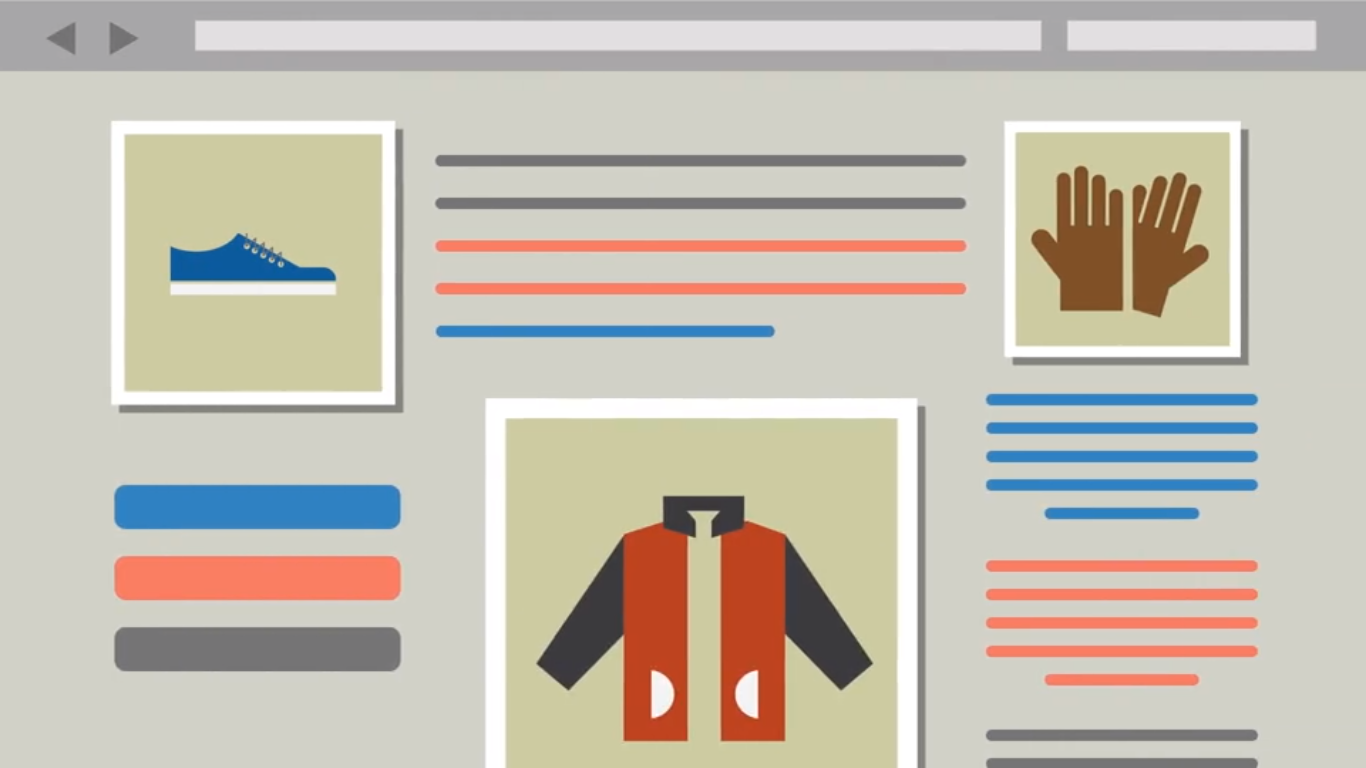
\includegraphics[width=10cm]{Resources/sort1.PNG}
	}
	\hspace{0mm}
	\subfloat[‌تبدیل محتوا به کارت‌های قابل مرتب‌سازی توسط کاربران و محول‌ کردن دسته‌بندی و مرتب‌سازی به کاربران سامانه به منظور تست و کشف الگوهای فکری کاربران‌]{
		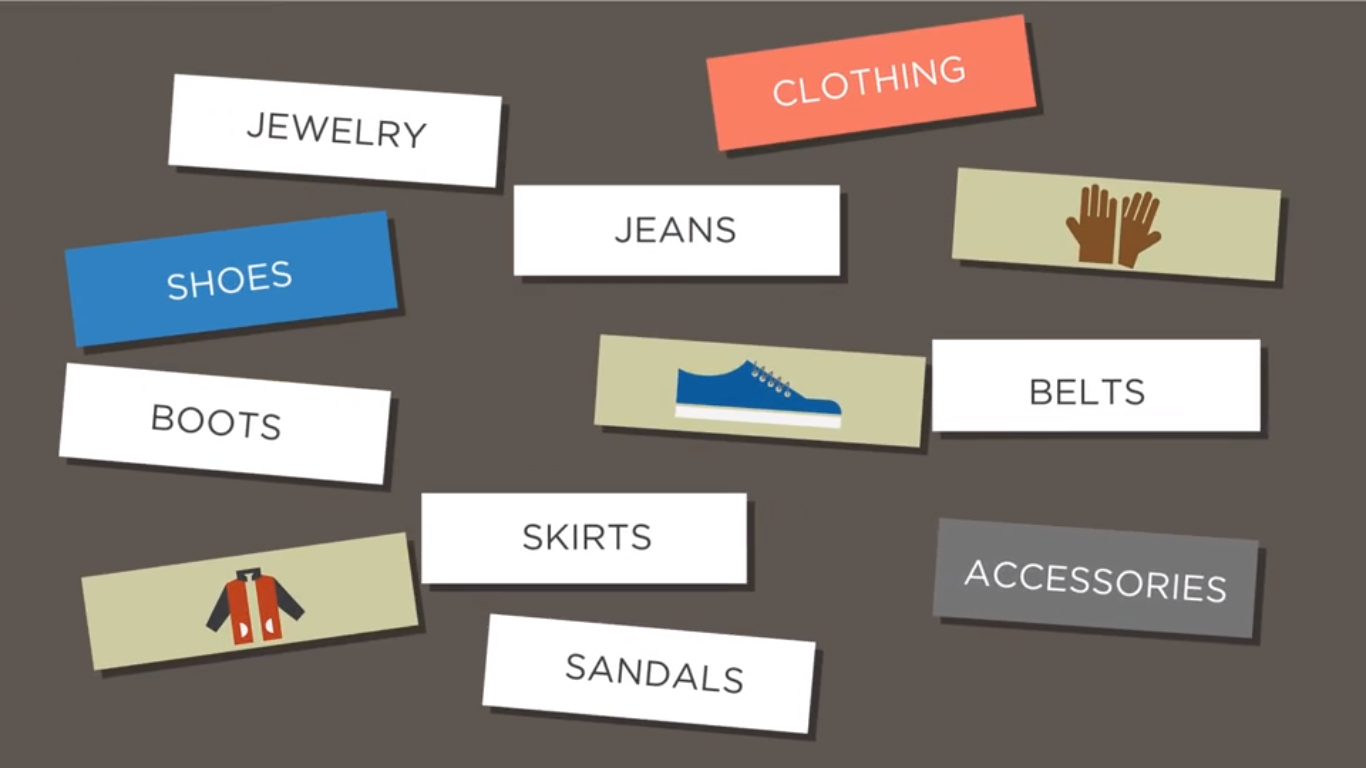
\includegraphics[width=10cm]{Resources/sort2.PNG}
	}
	\hspace{0mm}
	\subfloat[‌استفاده از الگوها و داده‌های استخراج شده از پاسخ کاربران در مرتب‌سازی کارت‌ها و نهایتا بهینه کردن ظاهر واسط کاربری‌]{
		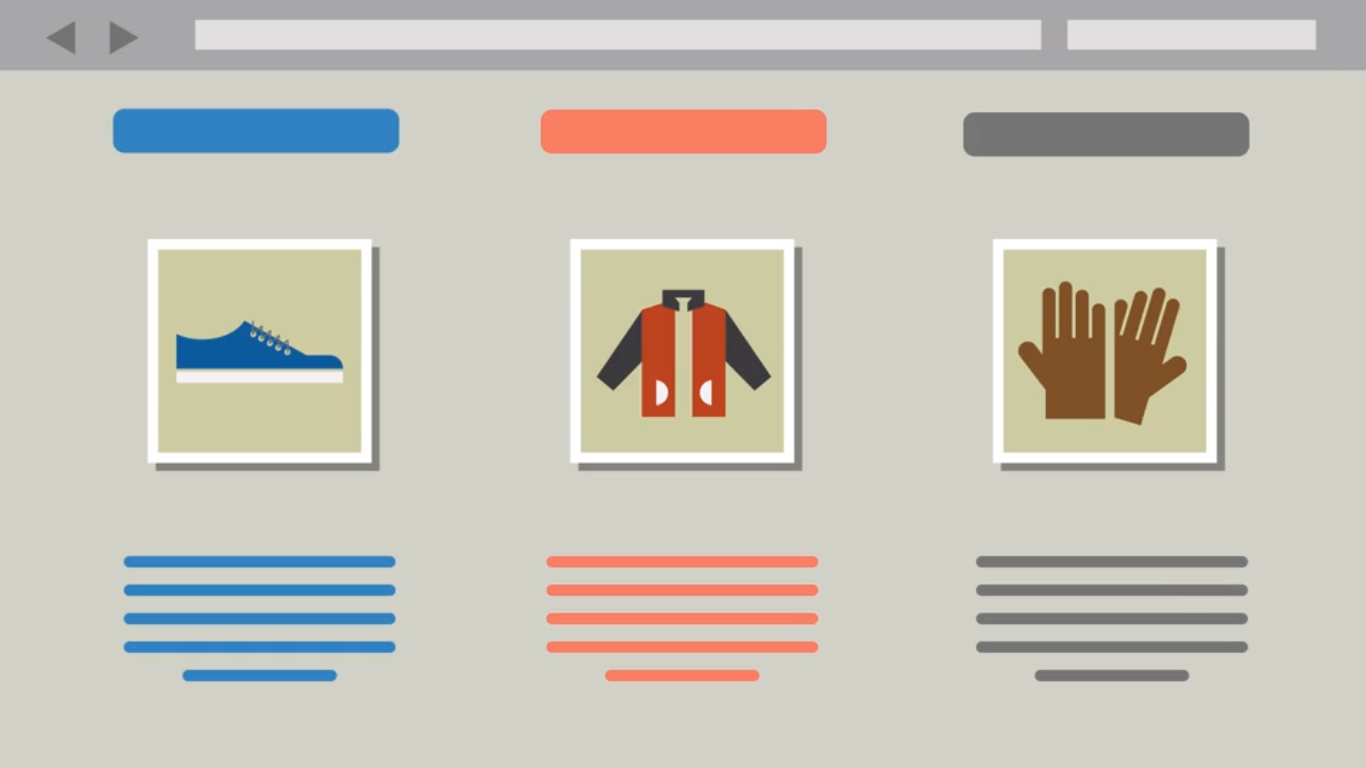
\includegraphics[width=10cm]{Resources/sort3.PNG}
	}
	\caption[تاثیر تست‌ها و الگوها مرتب‌سازی در استفاده‌پذیری]
	{تاثیر تست‌ها و الگوها مرتب‌سازی در استفاده‌پذیری
		\cite{noauthor_card_nodate}؛
		به منظور به دست آوردن داده‌های مرتب‌سازی، می‌بایست محتوای مورد نظر (آ) را در قالب کارت‌هایی درآورد  و سپس از شرکت‌کنندگان خواست که هرگونه که متمایل‌اند به مرتب‌سازی و دسته‌بندی این داده‌ها بپردازند. از پاسخ‌های برآمده از شرکت‌کنندگان می‌توان الگوهایی را استخراج کرد که بهینه‌ترین حالت چینش محتوا، از نظر کاربران، در رابط کاربری را می‌تواند نشان دهد (ج).
	}
	\label{fig:sorting}
\end{figure}
\section{روش‌های سنجش استفاده‌پذیری}
\begin{table}[H]
	\caption[بحث در مورد نحوه انجام مطالعه استفاده‌پذیری با توجه به روش‌های مختلف مطالعه]{
		بحث در مورد نحوه انجام مطالعه استفاده‌پذیری با توجه به روش‌های مختلف مطالعه
		\cite{albert_measuring_2013}
	}
	\label{tab:studies}
	\centering
	%	\resizebox{\textwidth}{!}{%
	\begin{tabular}{|C{5cm}|C{5cm}|}
		\hline
		\cellcolor{gray!25}
		‏ابتدا مطالعه آزمایشگاهی و سپس انجام مطالعه برخط
		&
		\cellcolor{gray!25}
		ابتدا مطالعه برخط و سپس مطالعه آزمایشگاهی	\\ \hline
		مشکلات ساده و کوچک را پیدا کرده یا حل می‌کنیم و بقیه مسائل و بحث‌ها به نمونه‌هایی با اندازه بزرگ‌تر سپرده می‌شود & ابتدا بزرگترین و اصلی‌ترین مشکلات را با داده‌های به دست آمده از مطالعه برخط، شناسایی می‌کنیم و سپس از مطالعات آزمایشگاهی استفاده می‌کنیم تا دانش کیفی بیشتری در مورد این مشکلات و مسائل به دست آوریم  \\ \hline
		راه‌حل‌ها، ایده‌ها و طرح‌های جدید با استفاده از تست آزمایشگاهی تولید می‌شوند و سپس توسط مطالعه برخط، مورد ارزیابی، سنجش و درستی‌آزمایی واقع می‌شوند & مصاحبه‌ها، تصاویر ویدیویی و نقل‌قول‌های مستقیم زیادی باید از کاربران جمع شود تا بتوان راه‌حل‌های جدید مطرح کرد و سپس در آزمایشگاه و در فضایی کوچکتر، با آن راه‌حل‌ها مسئله را حل کرد \\ \hline
		بازخورد کاربران و نحوه تعامل آن‌ها به صورت حضوری مورد بررسی و ارزیابی قرار می‌گیرد &  باید تمامی خصیصه‌ها در مورد کیفیت طراحی مورد پرسش و نظرسنجی قرار گیرند و اگر نتیجه نهایی مثبت بود، نیازی به انجام مطالعه آزمایشگاهی نیست \\ \hline
	\end{tabular}%
	%	}
\end{table}
به لطف فناوری وب و شبکه، امروزه محدود به یک روش سنجش و ارزیابی نیستیم. همانطور که از بررسی منابعی همچون
\cite{agarwal_assessing_2002}،
\cite{albert_measuring_2013}،
\cite{krug_dont_2018} و
\cite{noauthor_measuringu:_2018}
برمی‌آید، می‌توان خصیصه‌ها و اندازه‌گیری‌های مربوط به آن‌ها را تقریبا از هر روشی که ارزیابی بعدی از این داده‌ها را تضمین کند، به دست آورد. جمله پیشین به این معنی است که در مطالعه، سنجش و ارزیابی استفاده‌پذیری، نه تنها محدود به مشاهدات و آزمایشات آزمایشگاهی\RTLfootnote{
	به منظور مطالعه بیشتر می‌توان به مرجع
	\cite{li_crowdsourced_2016}
	مراجعه نمود که مروری روی انگیزه‌ها، روش‌ها و چالش‌های جمع‌سپاری می‌کند و از جمع‌سپاری به عنوان یک راه جمع‌آوری داده برای انجام ارزیابی‌ها و سنجش‌های مختلف نام می برد؛ در این منبع همچنین به دفعات متعدد اثبات شده است که هزینه استفاده از جمع‌سپاری برای جمع‌آوری داده به مراتب از روش‌هایی همچون روش‌های آزمایشگاهی کمتر بوده و با استفاده از این روش می‌توان با صرف زمان و هزینه کمتر، به نتایج گسترده‌تری رسید.
}
(که به معنای تعداد کم شرکت‌کنندگان و صرف زمان و هزینه زیاد است) نیستیم، بلکه می‌توانیم از روش‌هایی همچون مطالعات برخط استفاده کرده و حجم زیادی از تفاسیر و تحلیل‌ها را در زمان کمی به دست آوریم\RTLfootnote{
نکته قابل تامل از این نتیجه‌گیری این است که سازمان‌ها، کسب‌وکارها و شبکه‌های اجتماعی می‌توانند از قدرت کاربران خود استفاده کنند تا برای جمع‌آوری داده راهی هموارتر، که به دنبال آن سودآوری بیشتر خواهد آمد، داشته باشند. این به این معناست که همین پروژه می‌تواند در صورت پیاده‌سازی تجاری توسط یک سازمان دارای کسب‌وکاری از نوع
\lr{B2C (Business to Client)}
یک منبع درآمد اضافی باشد؛ کسب‌وکارهای نوپا
(\lr{Startups})
و سریس‌های مبتنی بر وب جدید را در نظر بگیرید. همه این کسب‌وکارها که سرویس خود را با کمک سامانه‌های مبتنی بر وب ارائه می‌دهند، همگی مایل‌اند که با صرف حداقل هزینه، به بهترین محصول برای شروع کسب‌وکار خود برسند. سازمان ارائه‌دهنده سرویس سنجش استفاده‌پذیری برای کسب‌وکارهای نوپا می‌تواند با استفاده از کاربران خود و با بهره‌گیری از روش‌های جمع‌سپاری و خرد‌کردن تست‌ها به میکرووظایف، داده‌های مربوط برای تست و سنجش استفاده‌پذیری محصولات نرم‌افزاری کسب‌وکارهای نوپا را فراهم کند. بنابراین این پروژه می‌تواند به عنوان یک طرح کسب‌وکاری
(\lr{Business Plan})
اولیه برای سازمان‌های درگیر با کاربران نهایی
(\lr{B2C})
و همچنین کسب‌وکارها
(\lr{B2B - Business to Business})
باشد.
}.\\
مطالعات برخط می‌توانند هم برای جمع‌آوری داده‌های کیفی و هم برای جمع‌آوری داده‌های کمی استفاده شوند؛ از طرفی دیگر در این نوع مطالعات می‌توان هم روی نگرش و هم روی رفتار شرکت‌کنندگان تامل کرد. به گفته مراجعی همچون
\cite{walker_high-fidelity_2002}
برخی از پژوهشگرانِ استفاده‌پذیری، ایده نوعی مطالعه ترکیبی را مطرح می‌کنند که در ادامه می‌توان به مطالعه برخط نیز آن را تعمیم داد. با در نظر گرفتن ایده‌های مختلفی، مرجع
\cite{albert_measuring_2013}
بررسی جامعی در مورد چگونگی مطالعه استفاده‌پذیری و در نهایت سنجش استفاده‌پذیری و جمع‌آوری داده و تحلیل آن‌ها انجام داده است که در جدول
\ref{tab:studies}
قابل مشاهده است.در این جدول یک نگاه کلی به دو روش شده است که الزاما نمی‌توان گفت کدام‌یک بهتر است\RTLfootnote{
	چرا که این مورد بسته به کاربرد بوده و در جایی که مثلا حل کردن مشکلات کوچک اهمیت زیادی دارد، می‌بایست در ابتدا مطالعه آزمایشگاهی و در مقیاس کوچک انجام دهیم؛ در موقعیتی هم که یافتن مسائل اصلی از اهمیت بالایی برخوردار است، می‌بایست از مطالعه برخط و سپس مطالعه آزمایشگاهی (به منظور ارائه راه‌حل) استفاده کنیم.
}؛ اما نکته حائز اهمیت این است که هر دو روش مطالعات برخط و آزمایشگاهی نقاط ضعف و قوت خود را دارند که می‌بایست در انجام مطالعات استفاده‌پذیری، این موارد و اینکه چگونه می‌توان از ترکیب هر دو نوع مطالعه بیشترین بازدهی را کسب کرد، در نظر گرفت. \\
در انجام مطالعه استفاده‌پذیری، 
بدیهی است که انجام مطالعه برخط، در صورت بهره‌ور نبودن، هزینه و زمان بسیاری را خواهد طلبید. همانطور که در بخش مقدمه مطرح شد، یکی از راه‌های کم‌هزینه برای جمع‌آوری داده زیاد با صرف هزینه کم و از طرفی بسیار قابل اطمینان
\cite{li_crowdsourced_2016}
، جمع‌سپاری است که در ساخت این ابزار نیز به عنوان یک روش اصلی برای مطالعه استفاده‌پذیری و پیدا کردن مشکلات اصلی استفاده‌پذیری در نظر گرفته شده است.
\section{ابزارهای مطالعه استفاده‌پذیری}
با بررسی‌های انجام شده از مهرماه سال ۱۳۹۶ تا زمان نگارش این اثر، بیش از ۸۰ ابزار، روش و تکنیک مطالعه و سنجش استفاده‌پذیری مورد بررسی موشکافانه قرار گرفتند که خلاصه این بررسی در جدول
\ref{tab:tools}
(رجوع شود به
\hyperref[sec:appendix]{پیوست})
قابل مشاهده است. لیست این ابزارها با مطالعه منابع برخط موجود و همچنین با فعالیت چند ساله نگارنده در حوزه توسعه سامانه‌های مبتنی بر وب متن‌باز و استفاده از منابع آکادمیک موجود تهیه شده است. با جمع‌آوری داده در مورد این ابزارها، شروع به بررسی نحوه سازوکار آن‌ها کردیم. در مورد برخی از این ابزارها که رایگان و یا متن‌باز بودند، بررسی و استفاده آن‌ها کار آسانی بود و با چندین نمونه آزمایشی توانستیم ویژگی‌های اصلی ابزار را شناسایی کنیم؛ در مورد قسمت دیگر ابزارها که به تمامی پولی بودند و یا استفاده از قسمتی از آن‌ها مستلزم پرداخت هزینه بود (نیمه رایگان)\RTLfootnote{
	اصطلاحا به این نوع استفاده،
	\lr{Freemium}
	گفته می‌شود که ترکیبی از دو لغت
	\lr{Premium}
	و
	\lr{Free}
	می‌باشد. در این حالت معمولا قسمتی از سرویس - که برای شروع به کار و یا استفاده اولیه می‌باشد - به صورت مجانی در دسترس بوده ولی مصرف‌کننده برای استفاده از ویژگی‌های دیگر ابزار می‌بایست هزینه خاصی را بپردازد و یا اشتراک خریداری کند.
}،
با استفاده از نقد و بررسی‌های موجود در سطح جوامع برخط و انجمن‌های گفتگو و همچنین دموها و اطلاعات موجود در وبسایت ابزارها که توسط سازندگان در دسترس عموم قرار گرفته بود، اطلاعات مربوط به نحوه کار و استفاده با ابزار را استخراج کردیم که در نهایت تمامی ابزارها را از لحاظ سناریوهای قابل انجام، بررسی نمودیم. شایان ذکر است که تعداد بسیار اندکی از ابزارهای مطرح (فقط یک ابزار که روی ردیابی چشم کاربر تاکید دارد) بر آزمایش‌های کوچک بسنده می‌کند و از جمع‌سپاری استفاده نمی‌کند؛ همچنین گفتنی است که هرکدام از این ابزارها، یا از سکوهای جمع‌سپاری\LTRfootnote{
	Crowdsourcing Platforms
} به منظور انجام جمع‌سپاری استفاده می‌کنند و یا خودشان با استفاده از قراردادهای داخلی، پلتفرم‌های خصوصی و یا سایر امکانات درون سازمانی خودشان، برای جمع‌آوری داده از روش جمع‌سپاری اقدامات لازم را انجام می‌دهند.\\
پیش‌تر ده سناریوی مهم برای بررسی و مطالعه استفاده‌پذیری مطرح شد که در جدول
\ref{tab:tools}،
در یک سو این سناریوها قابل مشاهده‌اند و در سویی دیگر ابزارها لیست شده‌اند. به منظور خلاصه‌سازی نتایج حاصل از این مطالعه، هرکدام از این ابزارها را برحسب نحوه کارکردشان و هدف نهایی هر کدام، در دسته‌هایی قرار می‌دهیم که الزاما هم از یکدیگر جدا نیستند؛ به عبارت دیگر، یک ابزار می‌تواند در دو یا چند دسته نیز قرار بگیرد.\\
	\begin{table}[H]
	\caption[دسته‌بندی ابزارهای مطرح در این پژوهش برای مطالعه استفاده‌پذیری]{
		دسته‌بندی ابزارهای در این پژوهش برای مطالعه استفاده‌پذیری؛ ابزارها مطابق با هدفی که هرکدام دنبال می‌کنند و نیز کارکردی که برای مصرف‌کنندگان دارند، در دسته‌هایی، که الزاما از یکدیگر انحصار ندارند، قرار گرفته‌اند.
	}
	\label{tab:tools_category}
	\centering
	\begin{tabular}{|C{3cm}|C{3.2cm}|C{3.2cm}|C{3.2cm}|C{0.8cm}|}
		\hline
		کارکرد و هدف نهایی & ورودی & نحوه کار & خروجی & تعداد ابزارها \\ \hline
		انتخابگر میان دو یا چند طرح & دو یا چندین طرح مفهومی/پیاده‌سازی‌شده مختلف & نمایش انتخاب‌های موجود به کاربر و دریافت پاسخ از وی و تجمیع داده‌ها & داده‌های تجمیع شده و نتیجه نهایی ترجیحات کاربران & 6 \\ \hline
		تحلیل‌گر & نقطه دسترسی به کل یا بخشی از سامانه & جمع‌آوری داده از روی پروفایل کاربران، تاریخچه کلیک‌ها، میزان وقت صرف شده در هر صفحه، موقعیت جغرافیایی و ... & تحلیل‌های پیشرفته از رفتار کاربران & 15 \\ \hline
		سنجش‌گر سازگاری با محیط‌های مختلف & نقطه دسترسی به کل یا بخشی از سامانه & بررسی نحوه رفتار سامانه  روی مرورگرها و سامانه‌های کاربری مختلف & مقدار سازگاری سامانه/صفحه مورد نظر با تغییرات محیطی & 4 \\ \hline
		ردیابی‌کننده  چشم کاربر & محیط آزمایشگاهی و کاربر مورد نظر برای تست & بررسی رفتار کاربر به واسطه حرکات چشم او & عملکرد رفتار کاربر در مواجهه با سامانه & 1 \\ \hline
		تولیدکننده نقشه حرارتی & نقطه دسترسی به کل یا بخشی از سامانه & جمع‌‌آوری داده‌های مربوط به کلیک‌های کاربران & نقشه‌های حرارتی که نشان‌دهنده نقاط با میزان توجه‌های متفاوت توسط کاربران است & 22 \\ \hline
		سنجش‌‌گر سرعت بارگزاری & نقطه دسترسی به کل یا بخشی از سامانه & دسترسی به سامانه در محیط‌ها و شرایط مختلف & کارایی و نحوه پاسخگویی سامانه & 5 \\ \hline
		پرسشنامه‌ساز & سوالات، موارد دارای ابهام و نظرسنجی‌های کیفیتی مطرح & پرسش از کاربران و شرکت‌کنندگان در نظرسنجی & پاسخ‌های تجمیع‌شده و تحلیلی از پاسخ‌های کاربران & 8 \\ \hline
		سنجش‌گر نمونه‌های مفهومی & نمونه‌های مفهومی و طرح‌های اولیه سامانه & طرح سوال از کاربران و درخواست انجام عملیات مشخص روی آن‌ها & نتایج تجمیع‌شده از میزان رضایت کاربران از طرح‌های اولیه و مفهومی & 20 \\ \hline
		سنجش‌گر کارایی کاربر & نقطه دسترسی به کل یا بخشی از سامانه & طرح پرسش‌هایی به منظور شروع تعامل کاربر و جمع‌آوری پاسخ کاربران & نتایج کارایی کاربران در تعامل با سامانه & 25 \\ \hline
		ثبت‌کننده عملیات کاربر & نقطه دسترسی به کل یا بخشی از سامانه & ردیابی حرکات کاربر و تعاملات وی با سامانه & نتایج تحلیل‌شده رفتار کاربر در تعامل با سامانه & 16 \\ \hline
		اعلام‌کننده بازخورد کاربر & نقطه دسترسی به کل یا بخشی از سامانه & طرح پرسش‌هایی به منظور شروع تعامل کاربر و جمع‌آوری پاسخ کاربران & تحلیل احساسات نهایی و امتیازات کاربر به سامانه & 7 \\ \hline
	\end{tabular}
\end{table}
مطابق جدول
\ref{tab:tools_category}
و البته شکل
\ref{fig:category_tools}
مشاهده می‌شود که بیشترین تمرکز در بین ابزارها، روی سنجش کارایی کاربران است که برای همین منظور، از تولید نقشه‌های حرارتی\LTRfootnote{Heatmaps} بهره برده می‌شود.\\
همچنین ملاحظه می‌شود که پس از موارد ذکر شده، سنجش و تست نمونه‌های مفهومی، از جمله هدف‌های محبوب ابزارها بوده است؛ البته با توجه به موارد ذکر شده در فصول پیشین و توجه به این نکته که افزایش استفاده‌پذیری طرح‌های مفهومی و اولیه، باعث کاهش هزینه‌ها و همچنین افزایش رضایت کاربری خواهد شد، می‌توانستیم از ابتدا نیز پیش‌بینی کنیم که رفع نواقص نمونه‌ها و طرح‌های اولیه از اهداف مهم ابزارها می‌باشد.\\
\begin{figure}[H]
	\centering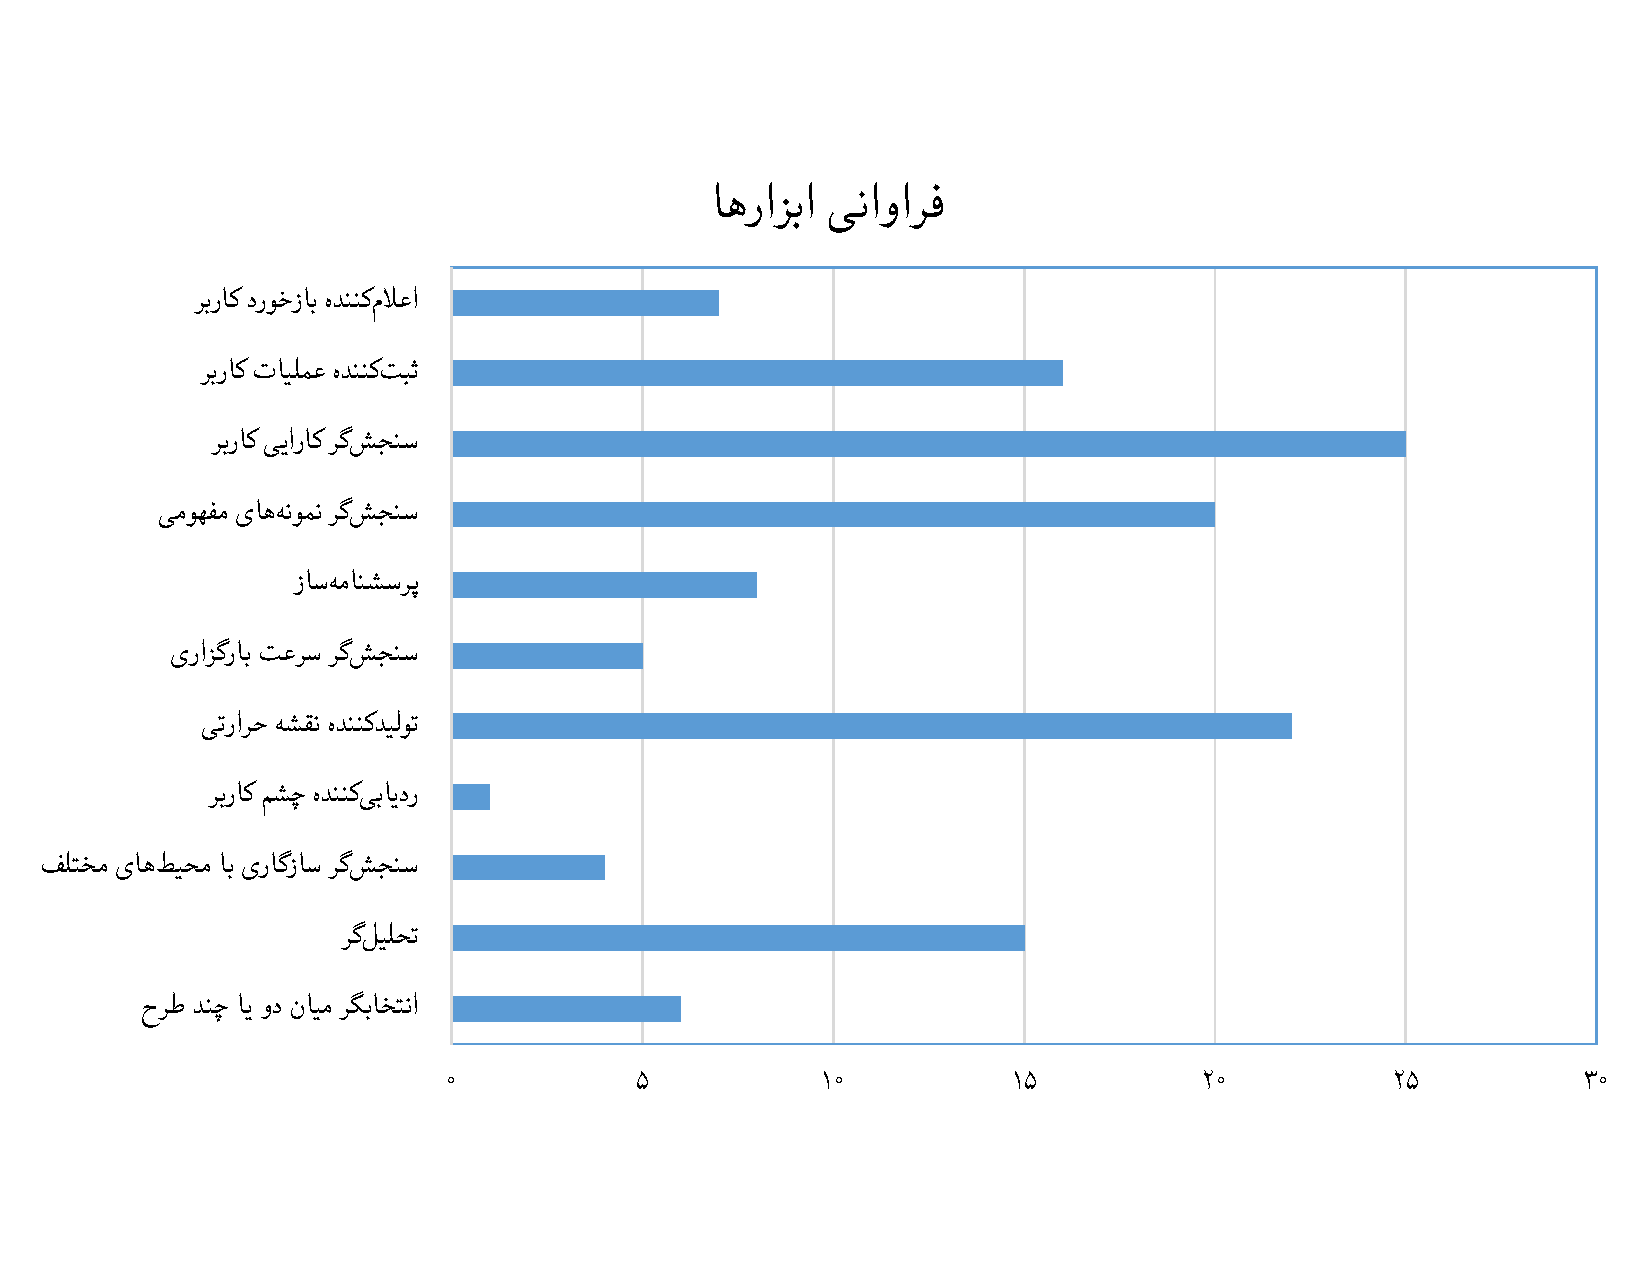
\includegraphics[width=0.8\linewidth]{Resources/tools_category.pdf}
	\caption[فراوانی ابزارهای موجود در هر دسته مطرح]
	{فراوانی ابزارهای موجود در هر دسته مطرح
	}
	\label{fig:category_tools}
\end{figure}
حال با شناخت اهداف هر کدام از این ابزارها، بد نیست به نحوه اندازه‌گیری خصیصه‌های کیفیتی مرتبط با استفاده‌پذیری در هر کدام بپردازیم. با بررسی این ۸۳ ابزار و با تجمیع داده‌های موجود در جدول
\ref{tab:tools}
می‌توان به یک سری الگوی تکراری در روش‌های اندازه‌گیری رسید که به طور کاملا مجزا و در ابزارهای متفاوتی دیده‌ می‌شوند. به منظور جمع‌آوری این الگو‌ها و بحث در مورد هر کدام، به بررسی موردی هرکدام از ابزارها پرداختیم؛ در این بررسی، سوال اصلی این بود که ابزار مورد نظر چگونه برای رسیدن به هدف مورد نظر و ماموریت خاص خود، به سنجش و اندازه‌گیری خصیصه‌های کیفیتی مرتبط با استفاده‌پذیری می‌پردازد؟\\
با استفاده از داده‌هایی که از ابزارهای مختلف داشتیم، سعی در نام‌گذاری برای هر الگوی مورد استفاده توسط گروهی از ابزارها کردیم. با در نظر گرفتن هدف هر ابزار و همچنین پاسخ دادن به سوال فوق در مورد هر ابزار، به نتایج بسیار جالبی رسیدیم که خلاصه آن‌ها در جدول
\ref{tab:scenario_measurement}
بیان شده است.
\begin{table}[H]
	\caption[
	فراوانی ابزارهای بررسی شده و الگوهای مورد استفاده توسط هرکدام
	]{
		فراوانی ابزارهای بررسی شده و الگوهای مورد استفاده توسط هرکدام؛ با استفاده از تجمیع داده‌های جدول
		\ref{tab:tools}
		ملاحظه می‌شود که به منظور انجام یکی از ده سناریوی مطرح در مطالعه استفاده‌پذیری، این ابزارها از الگوهای مشترک و مشخصی استفاده می‌کنند که می‌توان آن‌ها را در دسته‌های یکسان قرار داد.شایان ذکر است که طبق جدول
		\ref{tab:tools_category}،
		یک ابزار می‌تواند بیش از یک هدف و سناریو را مدنظر قرار دهد، به همین منظور دسته‌بندی این جدول، به طور کامل فضای ابزارهای مورد بررسی را افراز نمی‌کند و در نتیجه ابزارهایی را می‌توان یافت که از چندین الگو برای انجام یک یا چندین سناریو استفاده می‌کنند.
	}
	\label{tab:scenario_measurement}
	\begin{tabular}{|c|c|c|}
		\hline
		سناریوی مطرح & روش سنجش و اندازه‌گیری & فراوانی ابزارها \\ \hline
		\multirow{3}{*}{انجام یک تراکنش} & پرسشنامه متنی و تصویری & 7 \\ \cline{2-3} 
		& تست پیمایشی & 3 \\ \cline{2-3} 
		& ذخیره‌سازی کلیک‌های کاربران و پروفایل‌سازی & 14 \\ \hline
		\multirow{3}{*}{مقایسه محصولات} & تست ترجیح & 10 \\ \cline{2-3} 
		& تست‌های مرتبط با حافظه کوتاه‌مدت & 6 \\ \cline{2-3} 
		& پرسشنامه متنی و تصویری & 13 \\ \hline
		\multirow{3}{*}{ارزیابی استفاده مکرر از محصول} & ذخیره‌سازی کلیک‌های کاربران و پروفایل‌سازی & 6 \\ \cline{2-3} 
		& تست‌های مرتبط با حافظه کوتاه‌مدت & 6 \\ \cline{2-3} 
		& تست پیمایشی & 7 \\ \hline
		\multirow{4}{*}{ارزیابی پیمایش و معماری اطلاعات سامانه} & پرسشنامه متنی و تصویری & 9 \\ \cline{2-3} 
		& تست پیمایشی & 14 \\ \cline{2-3} 
		& استفاده از حسگر ردیاب چشم & 1 \\ \cline{2-3} 
		& ذخیره‌سازی کلیک‌های کاربران و پروفایل‌سازی & 8 \\ \hline
		\multirow{2}{*}{افزایش آگاهی} & پرسش سوالات مربوط به طرح‌های مفهومی & 7 \\ \cline{2-3} 
		& تست ترجیح & 5 \\ \hline
		\multirow{5}{*}{کشف مشکل} & بررسی فنی و جزئیات کد & 6 \\ \cline{2-3} 
		& ذخیره‌سازی کلیک‌های کاربران و پروفایل‌سازی & 9 \\ \cline{2-3} 
		& پرسش سوالات مربوط به طرح‌های مفهومی & 9 \\ \cline{2-3} 
		& استفاده از حسگر ردیاب چشم & 1 \\ \cline{2-3} 
		& پرسشنامه متنی و تصویری & 11 \\ \hline
		\multirow{3}{*}{حداکثرسازی استفاده‌پذیری یک محصول حیاتی} & استفاده از حسگر ردیاب چشم & 1 \\ \cline{2-3} 
		& تست ترجیح & 8 \\ \cline{2-3} 
		& ذخیره‌سازی کلیک‌های کاربران و پروفایل‌سازی & 4 \\ \hline
		\multirow{4}{*}{ایجاد تجربه کاربری مثبت} & پرسشنامه متنی و تصویری & 3 \\ \cline{2-3} 
		& تست ترجیح & 8 \\ \cline{2-3} 
		& پرسش سوالات مربوط به طرح‌های مفهومی & 7 \\ \cline{2-3} 
		& ذخیره‌سازی کلیک‌های کاربران و پروفایل‌سازی & 6 \\ \hline
		\multirow{6}{*}{ارزیابی تاثیرات تغییرات جزئی و نامحسوس} & بررسی فنی و جزئیات کد & 3 \\ \cline{2-3} 
		& استفاده از حسگر ردیاب چشم & 1 \\ \cline{2-3} 
		& تست ترجیح & 5 \\ \cline{2-3} 
		& ذخیره‌سازی کلیک‌های کاربران و پروفایل‌سازی & 9 \\ \cline{2-3} 
		& پرسشنامه متنی و تصویری & 7 \\ \cline{2-3} 
		& تست‌های مرتبط با حافظه کوتاه‌مدت & 6 \\ \hline
		\multirow{3}{*}{مقایسه طراحی‌های مختلف} & تست ترجیح & 10 \\ \cline{2-3} 
		& پرسش سوالات مربوط به طرح‌های مفهومی & 7 \\ \cline{2-3} 
		& پرسشنامه متنی و تصویری & 9 \\ \hline
	\end{tabular}
\end{table}
با مطالعه ابزارها و روش‌های موجود، الگوهای مشابهی از اعمال و راه‌حل‌ها برای حل مسائل مشاهده می‌شوند. مطابق جدول
\ref{tab:scenario_measurement}
هشت الگوی تکراری به منظور سنجش استفاده‌پذیری در این ابزارها دیده می‌شود که عبارتند از:
\begin{enumerate}
	\item
	پرسشنامه متنی و تصویری: در رابطه با یک یا چند تصویر مرتبط با یک طرح مفهومی یا نتیجه حاصل از یک کد، سوالاتی که اغلب پاسخ چند گزینه‌ای داشته، ولی می‌توانند پاسخ‌های کوتاه و بلند نیز داشته باشند، پرسیده می‌شود. در صورتی که پاسخ‌هایی غیر از چندگزینه‌ای از کاربران خواسته شود، می‌بایست پردازش‌های دیگری به منظور تحلیل دادگان آن‌ها انجام شود. البته باید توجه داشت که گاهی حتی سوالات به صورت تمام متنی هم هستند و ممکن است تصویری در پرسشنامه نباشد.
	\item 
	تست پیمایشی: با استفاده از طرح‌های مفهومی و یا صفحات اچ‌تی‌ام‌ال پیاده‌سازی شده، درخواست انجام یک یا چند عمل مشخص از کاربر می‌شود و پاسخ‌های وی با در نظر گرفتن زمان پاسخ ثبت می‌شوند.
	\item 
	ذخیره‌سازی کلیک‌های کاربران و پروفایل‌سازی: تمام تعاملات کاربر که از طریق دستگاه ورودی ماوس و حتی گاها کیبرد هستند، با رعایت ترتیب زمانی و زمان رخ‌داد، ذخیره شده و مورد بررسی و تحلیل واقع می‌شوند.
	\item 
	تست ترجیح: دو یا چند نمونه از طرح‌های اولیه و یا رابط‌های پیاده‌سازی شده به کاربر نمایش داده می‌شوند و از وی در مورد ترجیحاتش سوال پرسیده می‌شود.
	\item 
	تست‌های مرتبط با حافظه کوتاه مدت: به مدت محدودی، قسمتی از محتوا و یا واسط کاربری، مورد نمایش قرار می‌گیرد و پس از اتمام مهلت نمایش، از کاربر سوالاتی پرسیده می‌شود.
	\item 
	استفاده از حسگر ردیاب چشم:	این الگو که نوعی پروفایل‌سازی از کاربر است، با استفاده از تجهیزات اختصاصی و به منظور بررسی موشکافانه رفتار کاربر در تعامل با سیستم، انجام می‌شود. در نهایت از حسگر نیز به عنوان یک دستگاه ورودی استفاده شده است و تفاوت چندانی با حالت ذخیره‌سازی تعاملات با ماوس و کیبرد ندارد جز اینکه، جزئیات در اینجا بیشتر مورد توجه هستند.
	\item 
	پرسش سوالات مربوط به طرح‌های مفهومی: به طور خاص در مورد طرح‌های اولیه و خام و مفهومی که هنوز پیاده‌سازی نشده‌اند، سوالاتی از شرکت‌کننده پرسیده می‌شود.
	\item 
	بررسی فنی و جزئیات کد: در این الگو، به طور خاص، روی کد تولید شده تمرکز می‌شود و ابزار، اغلب به صورت اتوماتیک و صرفا با دریافت برخی از تنظیمات توسط کاربر، به بررسی جزئیات کد می‌پردازد. تمرکز اصلی در اینجا کشف خطاهای ناخواسته و غیرقابل تشخیص توسط انسان است که می‌تواند نقش شگرفی در افزایش استفاده‌پذیری بازی کند.
\end{enumerate}
با توجه به اطلاعات موجود در فصل‌های گذشته و با بررسی ابزارها، رویکردها و تکنیک‌های موجود در مطالعه استفاده‌پذیری، می‌توان گفت که هر ده سناریوی مطرح در مطالعه استفاده‌پذیری، از اهمیت خاصی برخوردارند که نمی‌توان منکر آن بود و در افزایش استفاده‌پذیری یک محصول، فارغ از ویژگی‌های تجاری محصول، تمامی سناریوها می‌بایست مورد نظر باشند. بنابراین با استفاده از مدل معرفی شده در منبع
\cite{albert_measuring_2013}
می‌بایست برای تمامی خصیصه‌های عنوان شده، یک یا چند روش اندازه‌گیری و یا زیرخصیصه مطرح کنیم که بتوانیم به پیاده‌سازی ابزاری کارا و موثر در مطالعه استفاده‌پذیری، بپردازیم. در فصل بعد به این مهم و همچنین ویژگی‌های ابزار هدف پرداخته‌ایم.

\chapter{ابزار هدف}
خصیصه‌های مطرح در مدل کیفیتی انتخاب شده، به طور خاص بیان‌گر نحوه اندازه‌گیری نیستند و می‌بایست به منظور رسیدن به یک ابزار درست، در ابتدا مدل‌ کیفیتی انتخاب شده را کمی شفاف‌تر کنیم تا نیازمندی‌ها به صورت دقیق‌تر مشخص شوند. به همین منظور می‌بایست تمامی یازده خصیصه کیفیتی مرتبط با استفاده‌پذیری را به تفصیل شرح داده و روش‌های اتخاذی خود را برای اندازه‌گیری هرکدام مطرح کنیم. از آن‌جا که هدف این پروژه تولید یک نرم‌افزار است، می‌بایست در قدم بعدی به بیان نمودارهای مرتبط بپردازیم و پس از پیاده‌سازی آزمایش‌های لازم را انجام داده و نتایج را ذکر کنیم. در طول این فصل به موارد ذکر شده پرداخته‌ایم که به ترتیب مورد بحث واقع شده‌اند.
\section{کشف نیازمندی‌ها}
ابزار مورد نظر می‌بایست قابلیت اندازه‌گیری استفاده‌پذیری در ذیل مدل کیفیتی مطرح شده در فصل پیشین (مدل تولیس
\cite{albert_measuring_2013})
را داشته باشد. بنابراین توجه به خصیصه‌های کیفیتی مطرح شده در این مدل، اولویت شماره اول است. بررسی مدل‌های کیفیتی مختلف (رجوع شود به جدول
\ref{tab:models})
بیانگر این است که در تبیین مدل‌های کیفیتی به دلیل کل‌نگر بودن و پرهیز از انحصاری شدن، می‌بایست تا حد امکان از بیان جزییات خصیصه‌ها خودداری کرد؛ اما در ساخت ابزارهای تست و سنجش کیفیت، بدون داشتن جزییات کافی از نحوه اندازه‌گیری، نخواهیم توانست که به سرمنزل مقصود برسیم. بنابراین می‌توان گفت که مهم‌ترین رسالت این پروژه، پر کردن خلا بین نیازمندی‌های نرم‌افزاری و مدل کیفیتی اتخاذ شده است.
\subsection{تجمیع نتایج پیشین و جمع‌بندی}
\begin{table}[H]
	\caption[
	تجمیع نتایج بررسی بهترین روش‌ها و ابزارها
	]{
		تجمیع نتایج بررسی بهترین روش‌ها و ابزارها؛ مطابق این تجمیع، مشاهده می‌شود که در ابزارها و روش‌ها و تکنیک‌های مطالعه استفاده‌پذیری، هشت الگوی تکراری، به منظور انجام ده سناریوی مهم در مطالعه استفاده‌پذیری استفاده شده‌اند.
	}
	\label{tab:tools_aggregated}
	\centering
	\begin{tabular}{|c|c|}
		\hline
		روش سنجش و اندازه‌گیری & دفعات تکرار الگو \\ \hline
		استفاده از حسگر ردیاب چشم & 4 \\ \hline
		بررسی فنی کد صفحات & 9 \\ \hline
		تست‌های مرتبط با حافظه کوتاه‌مدت & 18 \\ \hline
		تست پیمایشی & 24 \\ \hline
		پرسش سوالات مربوط به طرح‌های مفهومی & 30 \\ \hline
		تست ترجیح & 46 \\ \hline
		ذخیره‌سازی کلیک‌های کاربران و پروفایل‌سازی & 56 \\ \hline
		پرسشنامه متنی و تصویری & 59 \\ \hline
	\end{tabular}
\end{table}
با توجه به جدول
\ref{tab:scenario_measurement}
و همچنین نتایج ذکر شده در انتهای فصل پیشین، می‌توان به منظور درک اهمیت هرکدام از الگوها، مطالعه دیگری انجام داد؛ بد نیست به تجمیع داده‌های موجود در این جدول بیندیشیم. در این صورت به نتیجه بسیار جالب ذکر شده در جدول
\ref{tab:tools_aggregated}
خواهیم رسید که شکل
\ref{fig:tools_aggregation}
نیز بیانگر چهره دیگری از این جدول می‌باشد؛ بر اساس اطلاعات موجود در این شکل، ملاحظه می‌شود که دو الگوی بررسی فنی کد و استفاده از ردیاب، در تعداد کمی از مطالعات مورد استفاده قرار گرفته‌اند. در عمل، این دو الگو به خاطر بررسی مواردی خاص در نظر گرفته شده‌اند که در این موارد به منظور رسیدن به نتیجه‌ای مطلوب، می‌بایست از این‌چنین جزئیاتی نیز اطلاع داشته باشیم. اما نباید از این نکته غافل شد که این دو الگو نیازمند صرف وقت و هزینه بسیار زیادی می‌باشند؛ بدیهی است که برای ثبت داده‌های مربوط به نقطه تمرکز چشم کاربر، نیازمند شرایط، تجهیزات و فضای آزمایشگاهی خاص و گران قیمت خواهیم بود. همچنین به منظور بررسی دقیق و موشکافانه کد تولید شده نهایی، می‌بایست زمان زیادی را در ابتدا برای تولید ابزار طی کنیم که مطلوب ما نیست و می‌ةوان از سرویس‌هایی آماده و رایگانی همچون
\lr{Google Lighthouse}
استفاده کرد.
\begin{figure}[H]
	\centering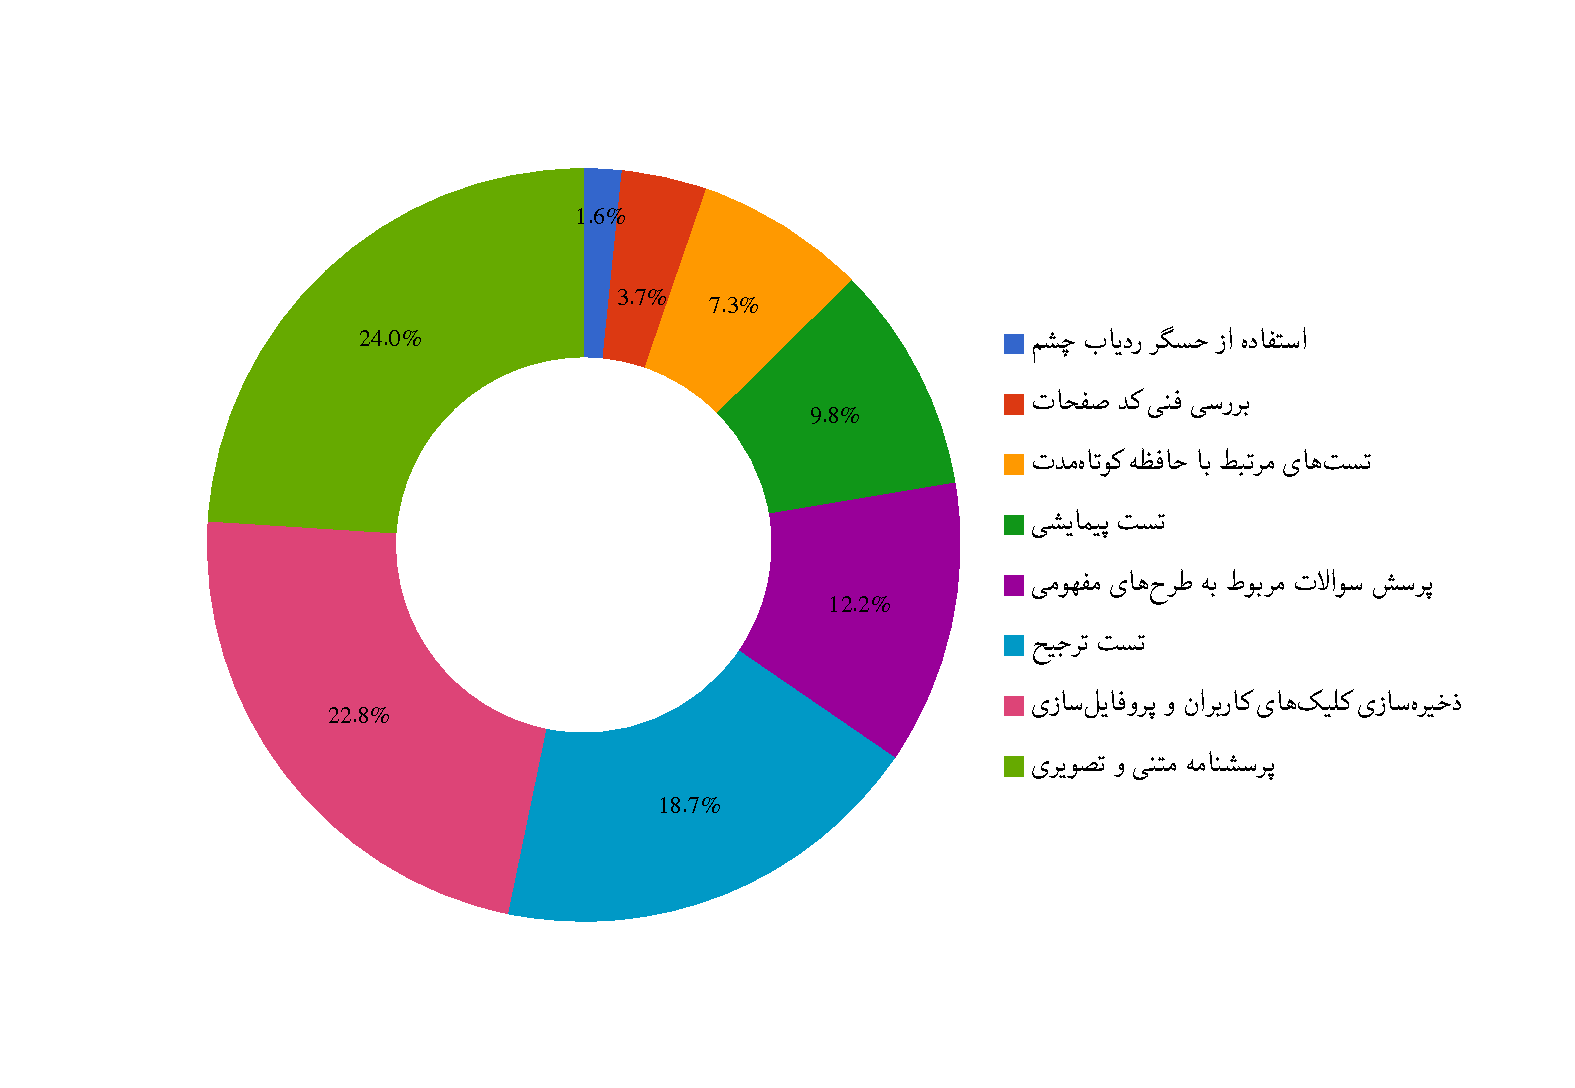
\includegraphics[width=\linewidth]{Resources/percentage.PNG}
	\caption[درصد فراوانی تکرار هر الگو در ابزارهای مورد بررسی]
	{درصد فراوانی تکرار هر الگو در ابزارهای مورد بررسی؛ مشاهده می‌شود که الگوهای ردیابی چشم و همچنین بررسی فنی کد، به دفعات کمتری مورد استفاده قرار گرفته‌اند چرا که کاربر بسیار محدود و جزئی‌ای در مطالعه استفاده‌پذیری دارند. در مقابل اما پرسشنامه‌ها و روش‌های پروفایل‌سازی بیشتر مطرح بوده‌اند.
	}
	\label{fig:tools_aggregation}
\end{figure}
\subsection{مهندسی نیازمندی‌ها}
حال به منظور مرور خصیصه‌های استفاده‌پذیری  و همچنین سناریوهای مطالعه استفاده‌پذیری و نیز اختصاص دادن یک شماره به هرکدام، در ادامه مجددا آن‌ها را یادآوری می‌کنیم؛ مطابق جدول
\ref{tab:10usability}،
سناریو‌های مطالعه استفاده‌پذیری و خصیصه‌های مورد توجه در هر کدام عبارتند از:
\begin{enumerate}
	\item
	انجام یک تراکنش: در این سناریو، خصیصه‌های «موفقیت آمیز بودن وظیفه»، «بهره‌وری کاربر»، «خصیصه‌های موردی»، «خصیصه‌های خود اعلامی» و همچنین «خصیصه‌های وبسایت بلادرنگ» می‌توانند مورد اندازه‌گیری و سنجش قرار می‌گیرند.
	\item
	مقایسه محصولات: با انجام این سناریو، می‌توان خصیصه‌های «موفقیت‌آمیز بودن وظیفه»، «بهره‌وری کاربر»، «خصیصه‌های خوداعلامی» و همچنین «خصیصه‌های ترکیبی و مقایسه‌ای» را مورد بررسی، سنجش و اندازه‌گیری قرار داد.
	\item
	ارزیابی استفاده مکرر از محصول: که در صورت انجام، «موفقیت‌آمیز بودن وظیفه»، «زمان انجام وظیفه»، «بهره‌وری»، «یادگیری‌پذیری» و نیز «خصیصه‌های خود اعلامی» را می‌توان مورد سنجش قرار داد.
	\item
	ارزیابی پیمایش و معماری اطلاعات سامانه: با اجرای این سناریو می‌توان «موفقیت‌آمیز بودن وظیفه»، «خطاها»، «بهره‌وری کاربر» و همچنین «الگوهای مرتب‌سازی» را مورد سنجش و ارزیابی قرار داد.
	\item
	افزایش آگاهی: با انجام مطالعه استفاده‌پذیری به منظور رسیدن به این هدف، می‌توان «خصیصه‌های خوداعلامی»، «خصیصه‌های فیزیولوژیکی و رفتاری» و همچنین «خصیصه‌های وبسایت‌ بلادرنگ» را مورد بحث و بررسی قرار داد.
	\item
	کشف مشکل: با در نظر قرار دادن این سناریو در انجام مطالعات استفاده‌پذیری، می‌توان «خصیصه‌های موردی» و «خصیصه‌های خوداعلامی» را مورد سنجش و ارزیابی قرار داد.
	\item 
	حداکثرسازی استفاده‌پذیری یک محصول حیاتی: هنگامی که این هدف مدنظر باشد، می‌توان «موفقیت‌آمیز بودن وظیفه»، «خطاها» و «بهره‌وری کاربر» را مورد توجه، سنجش و ارزیابی قرار داد.
	\item 
	ایجاد تجربه کاربری مثبت:
	در مطالعه استفاده‌پذیری به منظور ایجاد تجربه کاربری مثبت، «خصیصه‌های خوداعلامی» و همچنین «خصیصه‌های فیزیولوژیکی و رفتاری» که جزوی از ویژگی‌های کاربر نیز هستند، می‌توانند مورد توجه، ارزیابی و سنجش قرار بگیرند.
	\item 
	ارزیابی تاثیرات تغییرهای جزئی و نامحسوس: اگر مطالعه‌ای با این هدف انجام بگیرد، می‌تواند خصیصه‌ای همچون «خصیصه‌های وبسایت بلادرنگ» را با جزئیات زیادی مورد توجه خود واقع کند و به سنجش آن‌ها بپردازد.
	\item
	مقایسه طراحی‌های مختلف: که بیشتر به منظور بیشینه کردن راحتی کاربران هستند، می‌توانند برای سنجش و ارزیابی «موفقیت‌آمیز بودن وظیفه»‌، «زمان انجام وظیفه»، «خصیصه‌های موردی»، «خصیصه‌های خوداعلامی» و همچنین «خصیصه‌های ترکیبی و مقایسه‌ای» به کار گرفته شوند.
\end{enumerate}
\begin{table}[H]
	\caption[
	نیازمندی‌های کشف‌شده برای ابزار هدف
	]{
		نیازمندی‌های کشف‌شده برای ابزار هدف؛ این نیازمندی‌ها از روی الگوهای مطالعه و سنجش استفاده‌پذیری به دست آمده‌اند و طبق اطلاعات این جدول، به نظر می‌رسد که در صورت استفاده از این الگو، می‌توان بعد کاملی از مدل کیفیتی را، در مورد مطالعه استفاده‌پذیری، به کار برد. دقت شود که اعداد مربوط به سناریوهای مطالعه استفاده‌پذیری، اعداد ذکر شده در متن هستند.
	}
	\label{tab:requirements}
	\centering
	\begin{tabular}{|C{3cm}|C{3cm}|C{8cm}|}
		\hline
		الگو & سناریو(ها)ی قابل انجام & نیازمندی ابزار \\ \hline
		پرسشنامه متنی و تصویری & ۱، ۲، ۴، ۶، ۸، ۹، ۱۰ & دارا بودن امکان آپلود تصاویر و متون متعدد در قالب یک پرسشنامه و همچنین جمع‌آوری پاسخ کاربران \\ \hline
		ذخیره‌سازی کلیک‌های کاربران و پروفایل‌سازی & ۱، ۳، ۴، ۶، ۷، ۸ & استفاده از زبانی که به رخدادهای مرورگر پاسخ دهد \\ \hline
		تست ترجیح & ۲، ۵، ۷، ۸، ۹، ۱۰ & دارا بودن امکان آپلود تصاویر متعدد و نمایش آن‌ها در کنار هم و جمع‌آوری پاسخ کاربران \\ \hline
		پرسش سوالات مربوط به طرح‌های مفهومی & ۵، ۶، ۸، ۱۰ & دارا بودن امکان آپلود تصاویر و متون متعدد در قالب یک پرسشنامه و همچنین جمع‌آوری پاسخ کاربران \\ \hline
		تست پیمایشی & ۱، ۳، ۴ & دارا بودن امکان نمایش چندین عکس به طور متوالی و ذخیره پاسخ کاربر و زمان سپری شده توسط وی روی هرکدام \\ \hline
		تست‌های مرتبط با حافظه کوتاه مدت & ۲، ۳، ۹ & استفاده از زبانی که به رخدادهای مرورگر پاسخ دهد و همچنین قابلیت نمایش زمان‌دار موارد به کاربر \\ \hline
	\end{tabular}
\end{table}
با استفاده از اطلاعات ذکر شده و با توجه به تعریف‌هایی که از خصیصه‌های کیفیتی در فصل سوم مطرح شد، با نگاهی بر ابزارهای مطرح و روش‌های اندازه‌گیری آن‌ها و توجه به این نکته که این روش‌ها و ابزارها، در زمان نگارش این اثر، جزو بهترین روش‌ها\LTRfootnote{
	Best Practice
}
و ابزارهای موجود می‌باشند، می‌توان به طور خلاصه استراتژی مطرح برای اندازه‌گیری هر کدام از خصیصه‌ها را در قالب جدول
\ref{tab:requirements}
مطرح کرد؛ توجه به این نکته حائز اهمیت است که از دو الگوی هزینه‌بر ذکر شده صرف نظر شده است و نهایتا در ابزار هدف، به منظور اندازه‌گیری و سنجش خصیصه‌های کیفیتی مطرح شده در مدل تولیس، از ۶ الگوی مطرح شده در جدول
\ref{tab:requirements}،
استفاده می‌شود.\\
با توجه به پوشا بودن این نیازمندی‌ها\RTLfootnote{
	به این معنا که در صورت پیاده‌سازی شدن این نیازمندی‌ها، یک بعد از مدل کیفیتی که در مطالعات برخط می‌توان به آن‌ها پرداخت، به تمامی قابل حصول است و در واقع در مطالعه استفاده‌پذیری با این ابزار، می‌توان مطمئن شد که تمامی خصیصه‌های کیفیتی را می‌توان مورد سنجش و اندازه‌گیری قرار داد؛ چرا که طبق جدول‌های 
		\ref{tab:tools_category}
		و 
		\ref{tab:requirements}
		در صورت قادر بودن به انجام سناریوهای ذکر شده، می‌توان تمام خصیصه‌های مطرح در مدل کیفیتی را مورد سنجش و ارزیابی قرار داد.
}، می‌بایست به جنبه دیگر نیازمندی‌ها -نباید غافل شد که ما در پی ساخت ابزاری به منظور مطالعه استفاده‌پذیری به صورت برخط و با استفاده از جمع‌سپاری هستیم- پرداخت. با توجه به اینکه این ابزار در دسترس افراد زیادی خواهد بود، می‌بایست مدیریت حساب، احراز هویت، و حفظ حریم خصوصی افراد، به عنوان یک نیازمندی مهم مدنظر باشد؛ علاوه بر این موارد، می‌بایست تجمیع داده‌های حاصل از جمع‌سپاری به منظور تحلیل هرچه بهتر نتایج و همچنین پیاده‌سازی روش‌های جلوگیری از تاثیر اسپمرها می‌بایست در دستور کار قرار بگیرد.\\
\begin{figure}[H]
	\centering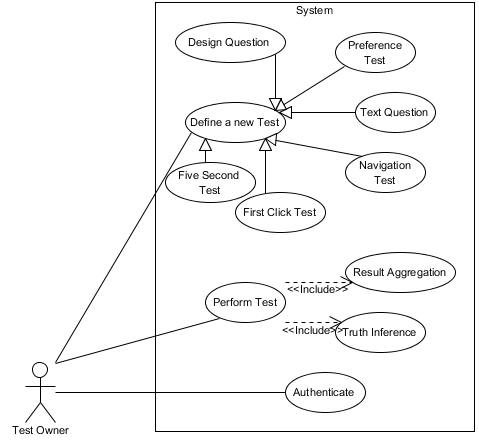
\includegraphics[width=\linewidth]{Resources/usecase_2.PNG}
	\caption[نمودار یوزکیس سامانه هدف]{
		نمودار یوزکیس سامانه هدف
	}
	\label{fig:usecase}
\end{figure}
با توضیحات پیشین، می‌توان نیازمندی‌های مطرح شده پیشین را به مدلی تبدیل کرد که در نمودار یوزکیس موجود در شکل
\ref{fig:usecase}،
قابل مشاهده است.
\section{توضیح کارکرد ابزار}
با کشف نیازمندی‌ها و پیاده‌سازی ابزار، صفحات پیاده‌سازی شده در سامانه کاربردی مبتنی بر وب (ابزار تست نهایی) به شرح زیر پیاده‌سازی شدند که کارکردهای اصلی در تصاویر موجود در شکل
\ref{fig:pages}
قابل مشاهده است.
\begin{figure}
	\centering
	\subfloat[فرم تعریف تست اولین کلیک]{
		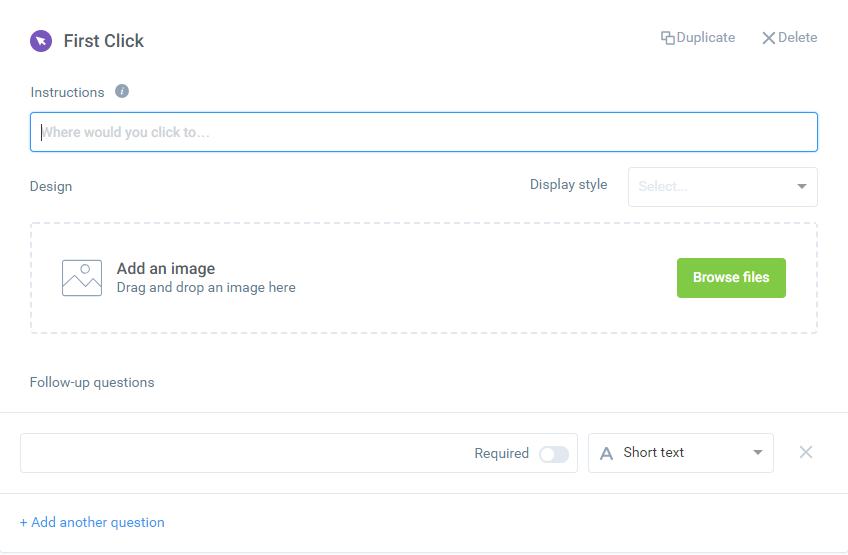
\includegraphics[width=6.5cm]{Resources/tool_1.PNG}
	}
	\subfloat[فرم تعریف تست پنج ثانیه]{
		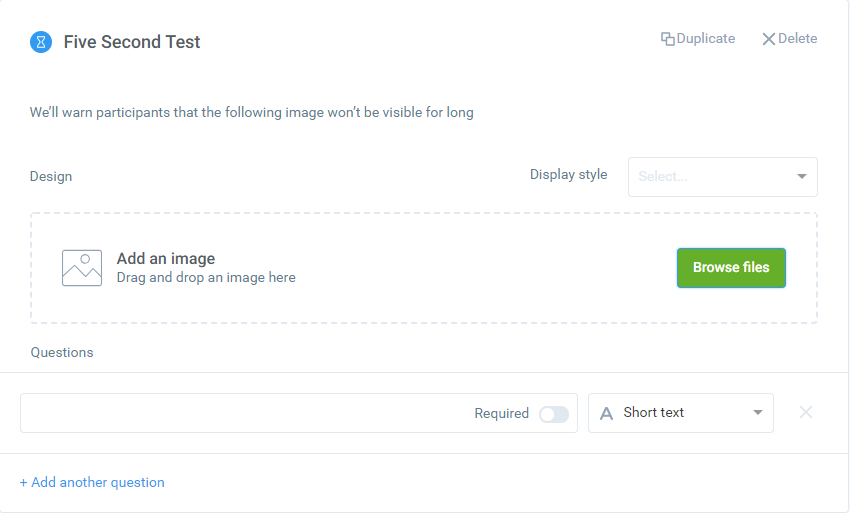
\includegraphics[width=6.5cm]{Resources/tool_2.PNG}
	}
	\hspace{0mm}
	\subfloat[فرم تعریف پرسشنامه متنی]{
		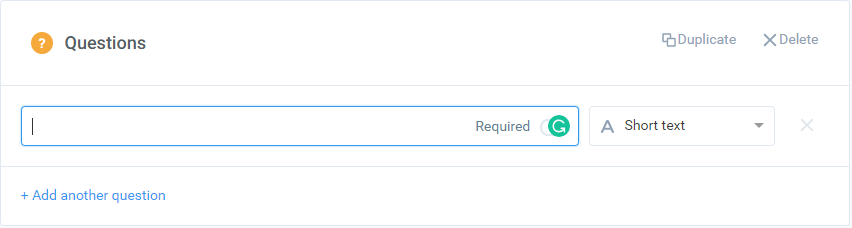
\includegraphics[width=6.5cm]{Resources/tool_3.PNG}
	}
	\subfloat[فرم تعریف پرسشنامه مربوط به طراحی (با عکس)]{
		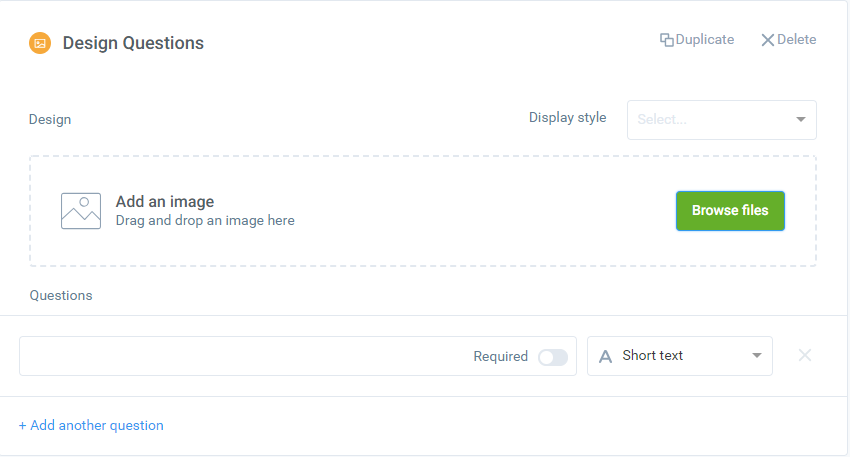
\includegraphics[width=6.5cm]{Resources/tool_4.PNG}
	}
	\hspace{0mm}
	\subfloat[فرم تعریف تست ترجیح]{
		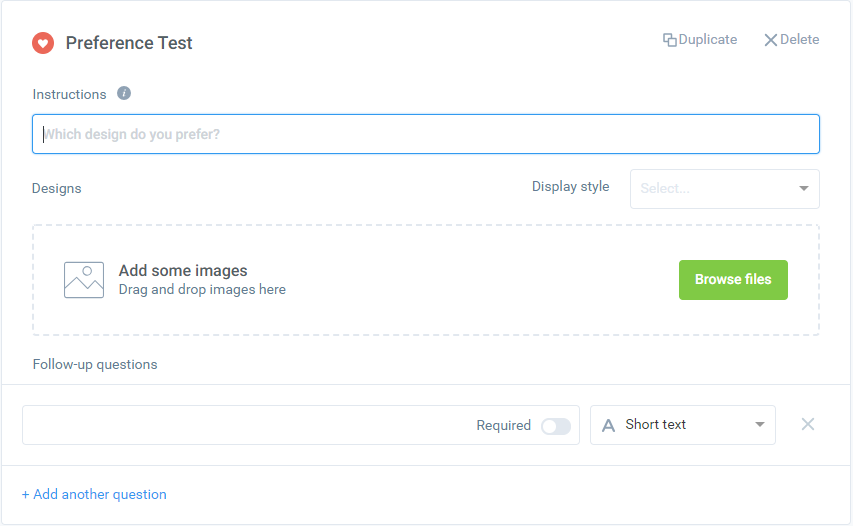
\includegraphics[width=6.5cm]{Resources/tool_5.PNG}
	}
	\subfloat[فرم تعریف تست پیمایش]{
		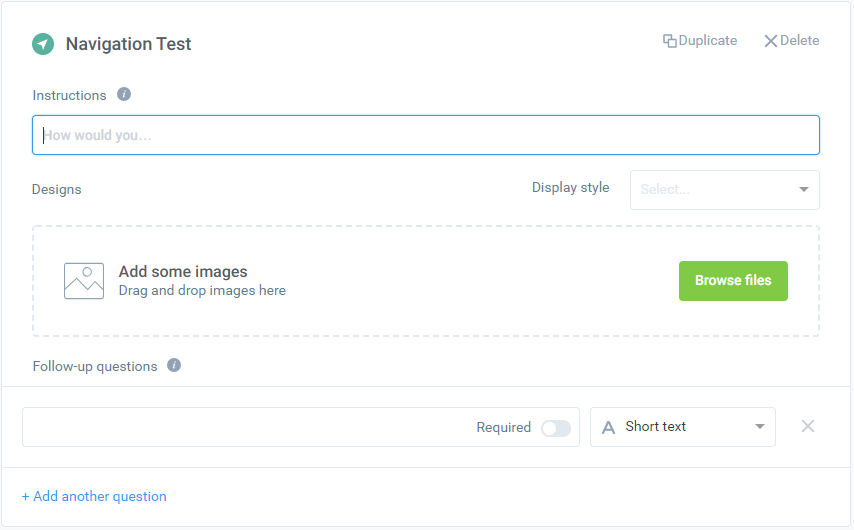
\includegraphics[width=6.5cm]{Resources/tool_6.PNG}
	}
	\caption[فرم‌های تعریف انواع تست‌های مختلف بر اساس الگوهای به دست آمده]
	{فرم‌های تعریف انواع تست‌های مختلف بر اساس الگوهای به دست آمده
	}
	\label{fig:pages}
\end{figure}
کاربران پس از ورود به حساب کاربری خود در سامانه، می‌توانند لیست تست‌های پیشین خود را مشاهده و در صورت لزوم در آن‌ها تغییری ایجاد کنند، حساب خود را مدیریت کنند و یا به ایجاد تست جدید بپردازند. پس از اینکه تست جدید ساخته شد و منتشر گردید، کاربر دارای آدرس وب منحصر به فردی خواهد شد که به طور خاص برای تست مدنظرش است؛ علاوه بر اینکه کاربر می‌تواند با به اشتراک گذاشتن آدرس وب با همگان، آن‌ها را دعوت به شرکت در انجام تست از طریق سامانه بکند، می‌تواند از امکان استفاده از سکوی جمع‌سپاری
\lr{Figure-Eight}\RTLfootnote{
	این سکو، درواقع همان سکوی
	\lr{CrowdFlower} می‌باشد که به تازگی و در سال ۲۰۱۸ تغییر نام داده و به 
	\lr{Figure-Eight}
	تبدیل شده است.
}
که با ابزار مورد نظر با واسط برنامه‌نویسی آن سکو ادغام شده است، بهره ببرد.\\
در هر دو صورت، داده‌های به دست آمده می‌بایست تجمیع شده و درستی و صحت آن‌ها تضمین شود. به منظور تضمین صحت و درستی داده‌ها، از روش تست پنهان استفاده می‌شود؛ همچنین گفتنی است که برای تجمیع داده‌ها و همچنین جلوگیری از تاثیر داده‌های هرز\LTRfootnote{Spam}، از روش کیفیت کارگران بهره گرفته می‌شود
\cite{li_crowdsourced_2016}.



















%\chapter{جمع‌بندي و نتيجه‌گيري و پیشنهادات}
%%%%%%%%%%%%%%%%%%%%%%%%%%%%%%%%%%%%%%%%%%%
در پايان گزارش‌هاي علمي و فني لازم است كه جمع‌بندي يا نتيجه‌گيري نهايي ارائه شود. در اين موارد مي‌توان آخرين فصل پایان نامه كه پیش از مراجع قرار مي‌گيرد را به اين امر اختصاص داد.
\section{پیشنهادات}
در این بخش پیشنهاداتی که محقق جهت ادامه تحقیقات دارد ارایه می‌گردد. دقت شود که پیشنهادات باید از  تحقیق انجام شده و نتایج ان حاصل شده باشد و از ذکر جملات کلی باید پرهیز کرد.

%--------------------------------------------------------------------------appendix( مراجع و پیوست ها)
\chapterfont{\vspace*{-2em}\centering\LARGE}%

\appendix
%\bibliographystyle{ieeetr-fa}
%\bibliography{survey2}
\begin{latin}
	\printbibliography[title=\rl{منابع و مراجع}]
\end{latin}

\chapter*{‌\rl{پیوست}}
\label{sec:appendix}
\markboth{\rl{پیوست}}{}
\addcontentsline{toc}{chapter}{\rl{پیوست}}
در این قسمت جداول و روابطی که، به خاطر طولانی بودن، در متن اصلی ذکر نشده‌اند درج شده است.
\newpage
\begin{longtable}{|c|C{3cm}|c|c|c|c|c|c|c|c|c|c|c|c|c|}
	\caption{مقایسه تطبیقی ابزارها و روش‌های موجود برای مطالعه استفاده‌پذیری}
	\label{tab:tools}\\
	\hline
	\multirow{2}{*}{\rotatebox{90}{ردیف}} &
	\multirow{2}{*}{نام ابزار} &
	\multirow{2}{*}{\rotatebox{90}{رایگان}} &
	\multirow{2}{*}{\rotatebox{90}{پولی}} &
	\multirow{2}{*}{\rotatebox{90}{نیمه رایگان}} &
	\multicolumn{10}{c|}{سناریوهای قابل انجام} \\ \cline{6-15} &
	&
	&
	&
	&
	\rotatebox{90}{انجام یک تراکنش} &
	\rotatebox{90}{مقایسه محصولات} &
	\rotatebox{90}{ارزیابی استفاده مکرر از محصول} &
	\rotatebox{90}{ارزیابی پیمایش و معماری اطلاعات سامانه} &
	\rotatebox{90}{افزایش آگاهی} &
	\rotatebox{90}{کشف مشکل} &
	\rotatebox{90}{حداکثرسازی استفاده‌پذیری یک محصول حیاتی}&
	\rotatebox{90}{ایجاد تجربه کاربری مثبت}&
	\rotatebox{90}{ارزیابی تاثیرات تغییرات جزئی و نامحسوس} &
	\rotatebox{90}{مقایسه طراحی‌های مختلف} \\ \hline
	\endfirsthead
	%
	
	%
	\hline
	\multicolumn{15}{| c |}{...ادامه جدول \ref{tab:tools}}\\
	\hline
	\multirow{2}{*}{\rotatebox{90}{ردیف}} &
	\multirow{2}{*}{نام ابزار} &
	\multirow{2}{*}{\rotatebox{90}{رایگان}} &
	\multirow{2}{*}{\rotatebox{90}{پولی}} &
	\multirow{2}{*}{\rotatebox{90}{نیمه رایگان}} &
	\multicolumn{10}{c|}{سناریوهای قابل انجام} \\ \cline{6-15} &
	&
	&
	&
	&
	\rotatebox{90}{انجام یک تراکنش} &
	\rotatebox{90}{مقایسه محصولات} &
	\rotatebox{90}{ارزیابی استفاده مکرر از محصول} &
	\rotatebox{90}{ارزیابی پیمایش و معماری اطلاعات سامانه} &
	\rotatebox{90}{افزایش آگاهی} &
	\rotatebox{90}{کشف مشکل} &
	\rotatebox{90}{حداکثرسازی استفاده‌پذیری یک محصول حیاتی}&
	\rotatebox{90}{ایجاد تجربه کاربری مثبت}&
	\rotatebox{90}{ارزیابی تاثیرات تغییرات جزئی و نامحسوس} &
	\rotatebox{90}{مقایسه طراحی‌های مختلف} \\ \hline
	\endhead
	%
	
	\multicolumn{15}{| c |}{ادامه جدول در صفحه بعد...}\\
	\hline
	\endfoot
	
	\multicolumn{15}{| c |}{انتهای جدول \ref{tab:tools}}\\
	\hline
	\endlastfoot
	
	1 & \lr{Ahrefs} &  & × &  &  &  &  & × & × & × &  & × &  &  \\ \hline
	2 & \lr{Browsershots} & × &  &  &  & × & × & × &  & × & × &  & × & × \\ \hline
	3 & \lr{Browserstack} &  & × &  &  & × & × & × &  & × & × &  & × & × \\ \hline
	4 & \lr{Bugsnag} &  &  & × & × &  & × &  & × & × &  &  & × &  \\ \hline
	5 & \lr{CheckMyColours} & × &  &  &  & × &  &  & × & × & × & × & × & × \\ \hline
	6 & \lr{ClickHeat} & × &  &  & × &  & × & × & × & × &  &  & × & × \\ \hline
	7 & \lr{Clicktale} &  & × &  & × &  & × & × & × & × &  & × &  & × \\ \hline
	8 & \lr{Clicky} &  &  & × & × &  & × & × & × & × &  &  & × & × \\ \hline
	9 & \lr{CrazyEgg} &  & × &  & × &  & × & × & × & × &  &  & × & × \\ \hline
	10 & \lr{CrazyEngage} & × &  &  &  & × &  &  & × &  & × &  & × & × \\ \hline
	11 & \lr{Critcue} &  &  & × & × &  & × & × & × & × & × & × &  &  \\ \hline
	12 & \lr{CrossBrowserTesting} &  & × &  &  & × & × & × &  & × & × &  & × & × \\ \hline
	13 & \lr{Ethnio} &  & × &  & × &  & × &  & × & × & × & × &  & × \\ \hline
	14 & \lr{Feng-GUI} &  & × &  &  & × & × & × & × &  & × &  & × & × \\ \hline
	15 & \lr{FullStory} &  &  & × &  &  & × & × & × &  & × & × &  &  \\ \hline
	16 & \lr{Google Analytics} &  &  & × & × &  & × & × &  & × &  &  & × & × \\ \hline
	17 & \lr{Google Forms} & × &  &  &  & × &  &  & × & × & × &  & × & × \\ \hline
	18 & \lr{Google Lighthouse} & × &  &  &  &  &  &  & × & × & × & × & × &  \\ \hline
	19 & \lr{Google Mobile Friendly Test} & × &  &  &  & × &  & × & × & × &  &  & × & × \\ \hline
	20 & \lr{Google PageSpeed Insight} & × &  &  &  & × & × &  & × & × & × &  &  & × \\ \hline
	21 & \lr{GTmetrix} &  &  & × &  & × & × &  & × & × & × &  &  & × \\ \hline
	22 & \lr{HEAT-MAP.co} &  &  & × & × &  & × & × & × & × &  &  & × & × \\ \hline
	23 & \lr{heatmap.me} &  &  & × & × &  & × & × & × & × &  &  & × & × \\ \hline
	24 & \lr{Hotjar} &  & × &  &  & × &  & × & × &  & × &  & × &  \\ \hline
	25 & \lr{Hoverowl} &  & × &  &  &  & × &  & × & × & × & × & × &  \\ \hline
	26 & \lr{Inspectlet} &  &  & × & × &  & × & × &  & × &  &  & × & × \\ \hline
	27 & \lr{iPerceptions} &  & × &  & × &  & × & × &  & × &  & × & × &  \\ \hline
	28 & \lr{Jaco} &  & × &  & × & × & × &  &  &  & × & × & × & × \\ \hline
	29 & \lr{Kampyle} &  & × &  & × &  & × & × & × & × &  &  & × & × \\ \hline
	30 & \lr{Koncept} &  & × &  & × & × & × & × & × & × & × & × & × & × \\ \hline
	31 & \lr{Loop11} &  & × &  & × & × & × & × & × & × &  & × & × & × \\ \hline
	32 & \lr{Lucky Orange} &  & × &  & × &  & × & × & × & × &  &  & × & × \\ \hline
	33 & \lr{Lytics} &  & × &  & × &  & × & × &  & × &  &  & × & × \\ \hline
	34 & \lr{Maze} &  & × &  & × &  & × & × &  &  & × & × & × & × \\ \hline
	35 & \lr{Mixpanel} &  &  & × &  & × & × &  & × & × &  & × & × & × \\ \hline
	36 & \lr{Morae} &  & × &  &  & × & × & × & × &  &  & × &  & × \\ \hline
	37 & \lr{Mouseflow} &  &  & × & × &  & × & × & × & × &  &  & × & × \\ \hline
	38 & \lr{MouseStats} &  &  & × & × &  & × & × & × & × &  &  & × & × \\ \hline
	39 & \lr{Moz} &  &  & × &  &  &  & × & × & × &  & × &  &  \\ \hline
	40 & \lr{Mr. Tappy} &  & × &  &  &  &  &  & × & × &  & × & × &  \\ \hline
	41 & \lr{Notable} &  & × &  & × &  &  & × & × & × & × &  & × & × \\ \hline
	42 & \lr{Omiconvert} &  & × &  & × & × &  & × &  &  &  &  & × & × \\ \hline
	43 & \lr{OpenHallway} &  &  & × &  & × & × & × & × &  &  &  & × & × \\ \hline
	44 & \lr{Optimal Workshop} &  &  &  & × &  & × &  & × &  & × & × &  &  \\ \hline
	45 & \lr{Optimizely} &  & × &  &  & × &  & × & × & × &  & × &  & × \\ \hline
	46 & \lr{Outsprung} &  & × &  &  &  & × & × & × & × &  & × & × &  \\ \hline
	47 & \lr{Ovo Studios} &  & × &  &  & × & × & × & × &  &  &  & × & × \\ \hline
	48 & \lr{Pingdom} &  & × &  &  &  &  &  & × & × & × & × & × &  \\ \hline
	49 & \lr{Ptengine} &  &  & × & × &  & × & × &  & × &  &  & × & × \\ \hline
	50 & \lr{Qualaroo} &  & × &  & × & × &  & × & × & × &  & × &  & × \\ \hline
	51 & \lr{ScreenLab} &  &  & × & × &  & × & × & × & × &  &  & × & × \\ \hline
	52 & \lr{SeeVolution} &  &  & × & × &  & × & × & × & × &  &  & × & × \\ \hline
	53 & \lr{SessionCam} &  &  & × & × & × &  & × & × &  &  &  & × & × \\ \hline
	54 & \lr{Simple Heatmaps} &  & × &  & × &  & × &  & × &  &  &  & × & × \\ \hline
	55 & \lr{SmartLook} &  &  & × & × &  & × & × & × & × & × &  & × & × \\ \hline
	56 & \lr{The User is Drunk} &  & × &  & × &  & × & × & × & × & × &  & × & × \\ \hline
	57 & \lr{The User is My Mom} &  & × &  & × &  & × & × & × & × & × &  & × & × \\ \hline
	58 & \lr{TruConversion} &  & × &  & × &  & × & × &  & × &  &  & × & × \\ \hline
	59 & \lr{TryMyUI} &  & × &  & × &  &  & × & × & × & × & × & × & × \\ \hline
	60 & \lr{UsabilityHub} &  &  & × & × &  & × & × & × &  &  &  & × & × \\ \hline
	61 & \lr{UsabilityTools} &  & × &  & × &  &  & × & × &  &  &  & × &  \\ \hline
	62 & \lr{Usabilla} &  & × &  & × & × &  & × & × &  &  &  & × & × \\ \hline
	63 & \lr{UserBob} &  & × &  &  &  & × & × & × & × &  &  & × &  \\ \hline
	64 & \lr{Userbrain} &  & × &  & × & × & × & × & × &  &  &  &  & × \\ \hline
	65 & \lr{Userfeel} &  & × &  & × &  & × & × &  & × & × & × & × & × \\ \hline
	66 & \lr{Userlytics} &  & × &  & × &  & × & × & × & × &  & × & × & × \\ \hline
	67 & \lr{Usersnap} &  & × &  & × &  & × & × & × & × &  &  & × & × \\ \hline
	68 & \lr{UserTesting} &  & × &  & × &  & × & × &  & × & × & × & × & × \\ \hline
	69 & \lr{UserTrack} &  & × &  & × & × &  & × & × & × & × &  & × & × \\ \hline
	70 & \lr{UserZoom} &  & × &  &  &  & × & × & × & × & × & × & × &  \\ \hline
	71 & \lr{UX Recorder} &  & × &  & × &  & × &  & × &  &  & × & × &  \\ \hline
	72 & \lr{Uxeria} &  & × &  & × & × & × & × & × &  &  & × &  & × \\ \hline
	73 & \lr{UXPin} &  & × &  & × & × & × & × & × & × &  & × & × & × \\ \hline
	74 & \lr{UXTesting} &  & × &  & × & × &  &  & × &  & × & × &  & × \\ \hline
	75 & \lr{Validately} &  & × &  & × &  & × &  & × &  & × & × & × &  \\ \hline
	76 & \lr{VerifyApp} &  & × &  & × & × &  & × & × & × & × & × &  & × \\ \hline
	77 & \lr{Visual Website Optimizer (VWO)} &  & × &  & × & × &  & × & × & × &  &  & × & × \\ \hline
	78 & \lr{Web Page Test} & × &  &  &  & × & × &  & × & × & × &  &  & × \\ \hline
	79 & \lr{Website Grader} & × &  &  &  & × & × & × &  & × & × &  & × &  \\ \hline
	80 & \lr{Weelytics} &  &  & × &  &  &  & × & × & × &  &  & × &  \\ \hline
	81 & \lr{WhatUsersDo} &  & × &  & × &  & × & × & × &  &  & × & × & × \\ \hline
	82 & \lr{Zarget} &  & × &  & × &  & × & × & × &  &  &  & × & × \\ \hline
	83 & \lr{Zeerat} &  &  & × & × &  & × &  & × & × & × & × & × & × \\ \hline
\end{longtable}
% براي شماره‌گذاري روابط، جداول و اشكال موجود در پيوست‌ از ساختار متفاوتي نسبت به متن اصلي استفاده مي‌شود كه در زير به‌عنوان نمونه نمايش داده شده‌است. 
% \begin{equation}
%F=ma
%\end{equation}
%--------------------------------------------------------------------------dictionary(واژه نامه ها)
%اگر مایل به داشتن صفحه واژه‌نامه نیستید، خط زیر را غیر فعال کنید.
\parindent=0pt
%
\chapter*{واژه‌نامه‌ی فارسی به انگلیسی}
\label{sec:glossary}
\pagestyle{style9}

\addcontentsline{toc}{chapter}{واژه‌نامه‌ی فارسی به انگلیسی}
%%%%%%
\begin{multicols*}{2}

{\bf الف}
\vspace*{3mm}
\farsiTOenglish{ارتباطاتی بودن}{Commucativeness}
\farsiTOenglish{ارزشیابی خرد}{Formartive Evaluation}
\farsiTOenglish{ارزشیابی کلان}{Summative Evaluation}
\farsiTOenglish{آزمون}{Test}
\farsiTOenglish{آسانی یادگیری}{Ease of Learning}
\farsiTOenglish{آستانه کیفیت}{Quality Threshold}
\farsiTOenglish{استفاده‌پذیری}{Usability}
\farsiTOenglish{استحکام}{Robustness}
\farsiTOenglish{اصلاح‌پذیری}{Modifiability}
\farsiTOenglish{الگو‌های مرتب‌سازی}{Card-Sorting Data}
\farsiTOenglish{آموزش}{Training}
\farsiTOenglish{ایمنی}{Safety}

\vspace*{3mm}
{\bf ب}
\vspace*{3mm}
\farsiTOenglish{بهره‌وری}{Efficiency}

\vspace*{3mm}
{\bf پ}
%%\vspace*{3mm}
\farsiTOenglish{پایا}{Invariant}

\vspace*{3mm}
{\bf ت}
%%\vspace*{3mm}
\farsiTOenglish{تاثیرگذاری}{Effectiveness}
\farsiTOenglish{ترابرپذیری}{Portability}
\farsiTOenglish{تناسب}{Approprateness}

\vspace*{3mm}
{\bf ث}
%%\vspace*{3mm}

\vspace*{3mm}
{\bf ج}
%%\vspace*{3mm}
\farsiTOenglish{جمع‌سپاری}{Crowdsourcing}

\vspace*{3mm}
{\bf چ}
%%\vspace*{3mm}

\vspace*{3mm}
{\bf ح}
%%\vspace*{3mm}

\vspace*{3mm}
{\bf خ}
%%\vspace*{3mm}
\farsiTOenglish{خاطرسپاری‌پذیری}{Memorability}
\farsiTOenglish{خصیصه کیفی}{Quality Metric}
\farsiTOenglish{خصیصه‌های ترکیبی و مقایسه‌ای}{Combined \& Comparative Metrics}
\farsiTOenglish{خصیصه‌های خوداعلامی}{Self-Reported Metrics}
\farsiTOenglish{خصیصه‌های فیزیولوژیکی و رفتاری}{Behavioral \& Physiological Metrics}
\farsiTOenglish{خصیصه‌های موردی}{Issue-Based Metrics}
\farsiTOenglish{خصیصه‌های وبسایت بلادرنگ}{Live Website Metrics}

\vspace*{3mm}
{\bf د}
%%\vspace*{3mm}
\farsiTOenglish{داده محک}{Benchmark}
\farsiTOenglish{دانایی‌پذیری}{Knowability}
\farsiTOenglish{درک‌پذیری}{Understandability}

\vspace*{3mm}
{\bf ذ}
%%\vspace*{3mm}

\vspace*{3mm}
{\bf ر}
%%\vspace*{3mm}
\farsiTOenglish{راحتی استفاده}{Ease of Use}
\farsiTOenglish{رضایت}{Satisfaction}
\farsiTOenglish{رضایت منحصر به فرد}{Subjective Satisfaction}

\vspace*{3mm}
{\bf ز}
%%\vspace*{3mm}
\farsiTOenglish{زیبایی}{Aesthetic}
\farsiTOenglish{زمان انجام وظیفه}{Task Time}

\vspace*{3mm}
{\bf ژ}
%%\vspace*{3mm}

\vspace*{3mm}
{\bf س}
%%\vspace*{3mm}
\farsiTOenglish{سازگاری}{Consistency}
\farsiTOenglish{سامانه کاربردی}{Application}
\farsiTOenglish{سامانه کاربردی تحت وب}{Web Application}

\vspace*{3mm}
{\bf ش}
%%\vspace*{3mm}
\farsiTOenglish{شناسایی‌پذیری}{Recognizability}

\vspace*{3mm}
{\bf ص}
%%\vspace*{3mm}
\farsiTOenglish{صادقانه}{Faithful}

\vspace*{3mm}
{\bf ض}
%%\vspace*{3mm}

\vspace*{3mm}
{\bf ط}
%%\vspace*{3mm}

\vspace*{3mm}
{\bf ظ}
%%\vspace*{3mm}

\vspace*{3mm}
{\bf ع}
%%\vspace*{3mm}
\farsiTOenglish{عملیاتی بودن}{Operability}

\vspace*{3mm}
{\bf غ}
%%\vspace*{3mm}

\vspace*{3mm}
{\bf ف}
%%\vspace*{3mm}
\farsiTOenglish{فرامدل}{Meta-Model}
\farsiTOenglish{فهم‌پذیری}{Comprehensibility}

\vspace*{3mm}
{\bf ق}
%%\vspace*{3mm}
\farsiTOenglish{قابلیت استفاده مجدد}{Reusability}

\vspace*{3mm}
{\bf ک}
%%\vspace*{3mm}
\farsiTOenglish{کارایی}{Performance}
\farsiTOenglish{کارگر جمع‌سپاری}{Crowd Worker}

\vspace*{3mm}
{\bf گ}
%%\vspace*{3mm}

\vspace*{3mm}
{\bf ل}
%%\vspace*{3mm}

\vspace*{3mm}
{\bf م}
%%\vspace*{3mm}
\farsiTOenglish{مفاد آموزشی}{Training Material}
\farsiTOenglish{مقیاس‌پذیری}{Scalability}
\farsiTOenglish{موفقیت‌آمیز بودن وظیفه}{Task Success}

\vspace*{3mm}
{\bf ن}
%%\vspace*{3mm}
\farsiTOenglish{نرخ بازگشت}{Bounce Rate}
\farsiTOenglish{نگرش مثبت}{Attitude}
\farsiTOenglish{نگه‌داری‌پذیری}{Maintainability}
\farsiTOenglish{نمودار فعالیت}{Activity Diagram}
\farsiTOenglish{نمودار مورد کاربرد}{Use Case Diagram}
\farsiTOenglish{نیمه‌رایگان}{Freemium}

\vspace*{3mm}
{\bf و}
%%\vspace*{3mm}
\farsiTOenglish{وظیفه}{Task}

\vspace*{3mm}
{\bf ه}
%%\vspace*{3mm}

\vspace*{3mm}
{\bf ی}
%%\vspace*{3mm}
\farsiTOenglish{یادگیری‌پذیری}{Learnability}
\end{multicols*}%
%%%%%%%
\chapter*{ واژه‌نامه‌ی انگلیسی به فارسی}
\pagestyle{style9}
\lhead{\thepage}\rhead{واژه‌نامه‌ی انگلیسی به فارسی}
\addcontentsline{toc}{chapter}{واژه‌نامه‌ی انگلیسی به فارسی}

\LTRmulticolcolumns
\begin{multicols}{2}
{\hfill\bf  \lr{A}}
%%\vspace*{1.5mm}

\englishTOfarsi{Automorphism}{خودریختی}

\vspace*{3mm}
{\hfill\bf   \lr{B}}
%%\vspace*{1.5mm}

\englishTOfarsi{Bijection}{دوسویی}

\vspace*{3mm}
{\hfill\bf   \lr{C}}
%%\vspace*{1.5mm}

\englishTOfarsi{Cycle group}{گروه دوری}

\vspace*{3mm}
{\hfill\bf   \lr{D}}
%%\vspace*{1.5mm}

\englishTOfarsi{Degree}{درجه}

\vspace*{3mm}
{\hfill\bf   \lr{E}}
%%\vspace*{1.5mm}

\englishTOfarsi{Edge}{یال}

\vspace*{3mm}
{\hfill\bf   \lr{F}}
%%\vspace*{1.5mm}

\englishTOfarsi{Function}{تابع}

\vspace*{3mm}
{\hfill\bf   \lr{G}}
%%\vspace*{1.5mm}

\englishTOfarsi{Group}{گروه}

\vspace*{3mm}
{\hfill\bf   \lr{H}}
%%\vspace*{1.5mm}

\englishTOfarsi{Homomorphism}{همریختی}

\vspace*{3mm}
{\hfill\bf   \lr{I}}
%%\vspace*{1.5mm}

\englishTOfarsi{Invariant}{پایا}

\vspace*{3mm}
{\hfill\bf   \lr{L}}
%%\vspace*{1.5mm}

\englishTOfarsi{Lift}{بالابر}

\vspace*{3mm}
{\hfill\bf   \lr{M}}
%%\vspace*{1.5mm}

\englishTOfarsi{Module}{مدول}

\vspace*{3mm}
{\hfill\bf   \lr{N}}
%%\vspace*{1.5mm}

\englishTOfarsi{Natural map}{نگاشت طبیعی}

\vspace*{3mm}
{\hfill\bf   \lr{O}}
%%\vspace*{1.5mm}

\englishTOfarsi{One to One}{یک به یک}

\vspace*{3mm}
{\hfill\bf   \lr{P}}
%%\vspace*{1.5mm}

\englishTOfarsi{Permutation group}{گروه جایگشتی}

\vspace*{3mm}
{\hfill\bf   \lr{Q}}
%%\vspace*{1.5mm}

\englishTOfarsi{Quotient graph}{گراف خارج‌قسمتی}

 \vspace*{3mm}
{\hfill\bf   \lr{R}}
%%\vspace*{1.5mm}

\englishTOfarsi{Reducible}{تحویل پذیر}

\vspace*{3mm}
{\hfill\bf   \lr{S}}
%%\vspace*{1.5mm}

\englishTOfarsi{Sequence}{دنباله}

 \vspace*{3mm}
{\hfill\bf   \lr{T}}
%%\vspace*{1.5mm}

\englishTOfarsi{Trivial character}{سرشت بدیهی}

\vspace*{3mm}
{\hfill\bf   \lr{U}}
%%\vspace*{1.5mm}

\englishTOfarsi{Unique}{منحصربفرد}

\vspace*{3mm}
{\hfill\bf   \lr{V}}
%%\vspace*{1.5mm}

\englishTOfarsi{Vector space}{فضای برداری}
\end{multicols}
%--------------------------------------------------------------------------index(نمایه)
%اگر مایل به داشتن صفحه نمایه نیستید، خط زیر را غیر فعال کنید.
%\pagestyle{style7}
%\printindex
\pagestyle{style7}
%کلمات کلیدی انگلیسی
\latinkeywords{Write a 3 to 5 KeyWords is essential. Example: AUT, M.Sc., Ph. D,..}
%چکیده انگلیسی

\en-abstract{
This page is accurate translation from Persian abstract into English.
}
%%%%%%%%%%%%%%%%%%%%% کدهای زیر را تغییر ندهید.

\newpage
\thispagestyle{empty}
\begin{latin}
\section*{\LARGE\centering Abstract}

\een-abstract

\vspace*{.5cm}
{\large\textbf{Key Words:}}\par
\vspace*{.5cm}
\elatinkeywords
\end{latin}
% در این فایل، عنوان پایان‌نامه، مشخصات خود و چکیده پایان‌نامه را به انگلیسی، وارد کنید.
%%%%%%%%%%%%%%%%%%%%%%%%%%%%%%%%%%%%
\baselineskip=.6cm
\begin{latin}

\latinfaculty{Department of Computer Engineering and Information Technology}


\latintitle{Implementing a Web Application to Test the Usability of Web Applications Using a Crwodsourced Approach}


\firstlatinsupervisor{Prof. Ahmad Abdollahzadeh Barforoush}

%\secondlatinsupervisor{Second Supervisor}

%\firstlatinadvisor{Dr. }

%\secondlatinadvisor{Second Advisor}

\latinname{Amir}

\latinsurname{HaghighatiMaleki}

\latinthesisdate{August 2018}

\latinvtitle
\end{latin}

\newpage
\end{document}